
%\documentclass[manuscript,screen,review]{acmart}
\documentclass[format=acmsmall, screen=true, review=false]{acmart}

%\documentclass[format=acmtog]{acmart}
%\documentclass[acmtog, review=false]{acmart}
%\usepackage[usenames]{color}
%\usepackage[table,dvipsnames]{xcolor}
\usepackage{soul}
%\usepackage{hyperref}
%\usepackage[bookmarks=false]{hyperref}
%\usepackage{amssymb}
\usepackage{makecell}
\usepackage{multirow}
\usepackage{enumitem}
\usepackage{array}
\usepackage{graphicx}
\usepackage{psfrag}
\usepackage{subfigure}
%\usepackage[pagebackref=true,breaklinks=true,linkcolor=red,anchorcolor=blue, citecolor=green,letterpaper=true,colorlinks,bookmarks=false]{hyperref}
\usepackage{bbding}
\usepackage{wrapfig}
\usepackage{url}
\usepackage{supertabular}
%\usepackage[graphicx]{realboxes}
\usepackage{adjustbox}
\usepackage{threeparttable}
\usepackage{tikz}
\usepackage{amsmath}
\usepackage{booktabs}
\usepackage{lscape}
\usepackage{verbatim}
\usepackage{longtable}
\usepackage{stfloats}
\usepackage[misc]{ifsym}
% \newcommand{\etal}{\textit{et al.}}
% \newcommand{\ie}{\emph{i.e., }}
% \newcommand{\eg}{\emph{e.g., }}
% \newcommand{\etc}{\emph{etc. }}
\usepackage{bm}
% \usepackage[cmintegrals]{newtxmath}
\usepackage{mathrsfs}
\usepackage[figuresright]{rotating}

\newtheorem{MyDef}{Definition}[subsection]
\newtheorem{MyTheory}{Theorem}
% \newtheorem{lemma}[theorem]{Theorem}
%\newtheorem{rmk}{Remark}
% \newtheorem{pf}{Proof}

% \usepackage{cite}
% \usepackage[UTF8]{ctex}
%\usepackage[colorlinks,linkcolor=blue]{hyperref}
%\usepackage[numbers,sort&compress]{natbib}

%% \BibTeX command to typeset BibTeX logo in the docs
\AtBeginDocument{%
  \providecommand\BibTeX{{%
    \normalfont B\kern-0.5em{\scshape i\kern-0.25em b}\kern-0.8em\TeX}}}

\usepackage{xspace}
\makeatletter 
% Add a period to the end of an abbreviation unless there's one
% already, then \xspace.
\DeclareRobustCommand\onedot{\futurelet\@let@token\@onedot}
\def\@onedot{\ifx\@let@token.\else.\null\fi\xspace}

\def\eg{\emph{e.g}\onedot} 
\def\Eg{\emph{E.g}\onedot}
\def\ie{\emph{i.e}\onedot} 
\def\Ie{\emph{I.e}\onedot}
\def\cf{\emph{c.f}\onedot} 
\def\Cf{\emph{C.f}\onedot}
\def\etc{\emph{etc}\onedot} 
\def\vs{\emph{vs}\onedot}
\def\wrt{w.r.t\onedot} 
\def\dof{d.o.f\onedot}
\def\etal{\emph{et al}\onedot}
\makeatother
%\newcommand{\zsf}[1]{\textcolor{red}{#1}}

%%%
%% The code below is generated by the tool at http://dl.acm.org/ccs.cfm.
%% Please copy and paste the code instead of the example below.
%%

\begin{CCSXML}
    <ccs2012>
       <concept>
           <concept_id>10003120.10003121.10011748</concept_id>
           <concept_desc>Human-centered computing~Empirical studies in HCI</concept_desc>
           <concept_significance>500</concept_significance>
           </concept>
       <concept>
           <concept_id>10003120.10003121.10003122.10011749</concept_id>
           <concept_desc>Human-centered computing~Laboratory experiments</concept_desc>
           <concept_significance>300</concept_significance>
           </concept>
       <concept>
           <concept_id>10010520.10010553.10010554</concept_id>
           <concept_desc>Computer systems organization~Robotics</concept_desc>
           <concept_significance>300</concept_significance>
           </concept>
     </ccs2012>
\end{CCSXML}
    
\ccsdesc[500]{Human-centered computing~Empirical studies in HCI}
\ccsdesc[300]{Human-centered computing~Laboratory experiments}
\ccsdesc[300]{Computer systems organization~Robotics}


%%
%% Keywords. The author(s) should pick words that accurately describe
%% the work being presented. Separate the keywords with commas.
\keywords{synchronization, trust, non-humanoid robot, dynamical approach, design strategy}

%% Rights management information.  This information is sent to you
%% when you complete the rights form.  These commands have SAMPLE
%% values in them; it is your responsibility as an author to replace
%% the commands and values with those provided to you when you
%% complete the rights form.
\setcopyright{acmcopyright}
%\copyrightyear{2022}
%\acmYear{2022}
% \acmDOI{XXXXXXX.XXXXXXX}

%%
%% These commands are for a JOURNAL article.
\acmJournal{CSUR}
% \acmVolume{37}
% \acmNumber{4}
% \acmArticle{111}
% \acmMonth{8}

%% These commands are for a PROCEEDINGS abstract or paper.
%\acmConference[Conference acronym 'XX]{Make sure to enter the correct
%  conference title from your rights confirmation emai}{June 03--05,
%  2018}{Woodstock, NY}
%\acmPrice{15.00}
%\acmISBN{978-1-4503-XXXX-X/18/06}


%%
%% Submis

\hyphenpenalty=8000
\tolerance=3000
%% end of the preamble, start of the body of the document source.
\begin{document}

%%
%% The "title" command has an optional parameter,
%% allowing the author to define a "short title" to be used in page headers.

\title{Deep Learning for Cross-Domain Few-Shot Visual Recognition: A Survey}



% \title{Cross-Domain Few-Shot Learning: A Survey}
%%
%% The "author" command and its associated commands are used to define
%% the authors and their affiliations.
%% Of note is the shared affiliation of the first two authors, and the
%% "authornote" and "authornotemark" commands
%% used to denote shared contribution to the research.
\author{Huali Xu}
\email{huali.xu@oulu.fi}
\affiliation{%
  \institution{CMVS, University of Oulu}
  \streetaddress{Pentti Kaiteran katu 1}
  \city{Oulu}
  \state{Oulu}
  \country{Finland}
  \postcode{90570}
}

\author{Shuaifeng Zhi*}  % \authornote{*Corresponding author}
% \cortext[mycorrespondingauthor]{Corresponding author}
\affiliation{%
  \institution{National University of Defense Technology}
  \city{Changsha}
  \state{Hunan}
  \country{China}}
\email{zhishuaifeng@outlook.com}

\author{Shuzhou Sun}
\email{shuzhou.sun@oulu.fi}
\affiliation{%
  \institution{CMVS, University of Oulu}
  \streetaddress{Pentti Kaiteran katu 1}
  \city{Oulu}
  \state{Oulu}
  \country{Finland}
  \postcode{90570}
}

\author{Vishal M. Patel}
\affiliation{%
  \institution{Johns Hopkins University}
  \streetaddress{3400 N. Charles Street}
  \city{Baltimore}
  \state{Maryland}
  \country{USA}
}
\email{vpatel36@jhu.edu}

\author{Li Liu}   \authornote{Corresponding author}
% \corref{mycorrespondingauthor}
\affiliation{
  \institution{College of Electronic Science, National University of Defense Technology}
  \city{Changsha}
  \state{Hunan}
  \country{China}}
\affiliation{
  \institution{CMVS, University of Oulu}
  \streetaddress{Pentti Kaiteran katu 1}
  \city{Oulu}
  \state{Oulu}
  \country{Finland}
  \postcode{90570}}
\email{li.liu@oulu.fi}



%%
%% By default, the full list of authors will be used in the page
%% headers. Often, this list is too long, and will overlap
%% other information printed in the page headers. This command allows
%% the author to define a more concise list
%% of authors' names for this purpose.
\renewcommand{\shortauthors}{Huali Xu, Shuaifeng Zhi, Shuzhou Sun, Vishal M. Patel and Li Liu}

%\renewcommand{\shortauthors}{Huali Xu, Shuaifeng Zhi, Vishal M. Patel and Li Liu, et al.}

%%
%% The abstract is a short summary of the work to be presented in the
%% article.
\begin{abstract}
Deep learning has been highly successful in computer vision with large amounts of labeled data, but struggles with limited labeled training data. To address this, Few-shot learning (FSL) is proposed, but it assumes that all samples (including source and target task data, where target tasks are performed with prior knowledge from source ones) are from the same domain, which is a stringent assumption in the real world. To alleviate this limitation, Cross-domain few-shot learning (CDFSL) has gained attention as it allows source and target data from different domains and label spaces. This paper provides a comprehensive review of CDFSL at the first time, which has received far less attention than FSL due to its unique setup and difficulties. We expect this paper to serve as both a position paper and a tutorial for those doing research in CDFSL. This review first introduces the definition of CDFSL and the issues involved, followed by the core scientific question and challenge. A comprehensive review of validated CDFSL approaches from the existing literature is then presented, along with their detailed descriptions based on a rigorous taxonomy. Furthermore, this paper outlines and discusses several promising directions of CDFSL that deserve further scientific investigation, covering aspects of problem setups, applications and theories.
% In recent years, deep learning has been highly successful in computer vision, by leveraging large amounts of supervised data but it often fails when the data set is small. Few-shot learning (FSL), aimed at solving a target task with only very limited supervised information available, is proposed to address this problem.
% However, deep learning based methods usually do not perform well and even worse than traditional machine learning algorithms when there are no enough supervised samples. Based on this problem, researchers study a new problem, which is few-shot learning. 
%Few-shot learning aims at solving a target task with only very limited supervised information available. 
% However, FSL assumes that all samples are i.i.d., which is a very strict assumption in the real world. To tackle this problem, Cross-Domain Few-Shot Learning (CDFSL) is studied in recent years. CDFSL leverages prior knowledge learned from a supervised auxiliary dataset to solve a target task with limited supervised information available, where the auxiliary datasets and target datasets come from two different domains and different label spaces. These procedures are of both practical and theoretical importance, as they are crucial for many realistic scenarios in which data is either costly or even impossible to retrieve. Furthermore, they alleviate the limitation of requiring the auxiliary data that come from the same domain with target data in few-shot task. This survey, to our best knowledge, is the first work focusing on the topic of cross-domain few-shot learning, which has received far less attention compared to few-shot learning due to its unique challenges. This survey provides an extensive overview and detailed description of approaches which have been validated from the current literature, and classifies these works according to a strict taxonomy. Furthermore, we also review and discuss the advantages and disadvantages of each category. Besides, the promising directions of challenges, techniques, and applications in CDFSL are also proposed to provide insights for future research.

\end{abstract}

%%
%% The code below is generated by the tool at http://dl.acm.org/ccs.cfm.
%% Please copy and paste the code instead of the example below.
%%
\begin{CCSXML}
<ccs2012>
   <concept>
       <concept_id>10010147.10010257.10010258.10010259.10010263</concept_id>
       <concept_desc>Computing methodologies~Supervised learning by classification</concept_desc>
       <concept_significance>500</concept_significance>
       </concept>
   <concept>
       <concept_id>10010147.10010257.10010258.10010259.10010263</concept_id>
       <concept_desc>Computing methodologies~Supervised learning by classification</concept_desc>
       <concept_significance>100</concept_significance>
       </concept>
 </ccs2012>
\end{CCSXML}

\ccsdesc[500]{Computing methodologies~Supervised learning by classification}
\ccsdesc[100]{Computing methodologies~Supervised learning by classification}


%%
%% Keywords. The author(s) should pick words that accurately describe
%% the work being presented. Separate the keywords with commas.
\keywords{Deep Learning, Computer Vision, Cross-Domain Few-Shot Learning, Literature Survey}


%%
%% This command processes the author and affiliation and title
%% information and builds the first part of the formatted document.
\maketitle

\section{Introduction}
Deep learning~\cite{dl} has been highly successful in computer vision~\cite{sg1,od1,app-detection,zhou2024diffdet4sar,li2024predicting,yang2024saratr,LiSARATRX25}, largely due to the availability of large-scale labeled datasets. However, in many practical scenarios, obtaining such large amounts of labeled data is difficult or costly. To address this challenge, Few-shot learning (FSL) aims to enable models to learn new tasks with only a limited number of labeled samples. Consequently, this problem has garnered significant attention in both academia and industry due to its broad real-world applications. While humans can easily distinguish between objects after seeing only a few examples, machines struggle to achieve similar efficiency. In domains such as natural scene images, large datasets are readily available, but FSL is crucial in scenarios where collecting large amounts of data is difficult. Since the problem was first introduced in 2006~\cite{fsl-1}, numerous methods have been proposed to tackle the challenges of FSL~\cite{fslsurvey,fslsurvey22,fslsurvey20,fsl18,fslsurvey1}.

With the development of FSL, challenges such as limited training data, domain variations, and task modifications have led to the emergence of various FSL variants, including semi-supervised FSL~\cite{semifsl}, unsupervised FSL~\cite{ufsl1,ufsl2}, zero-shot learning (ZSL)\cite{zsl1}, and cross-domain FSL (CDFSL)~\cite{feature-wise,bscd-fsl}, among others. These variants represent distinctive cases of FSL in terms of sample availability and domain learning. This paper focuses specifically on CDFSL variants. The traditional FSL problem assumes that both prior knowledge and target tasks come from the same domain, which is often restrictive in real-world applications. CDFSL addresses this issue by overcoming the domain gap between auxiliary data (which provides prior knowledge) and the target data in FSL tasks, as show in Figure~\ref{int}. For instance, in art image recognition tasks involving scribble, cartoon, or sketch images, FSL could theoretically leverage prior knowledge from related domains like cartoons and sketches. However, such data is often scarce due to copyright restrictions and the high cost of collection. As a result, researchers have turned to data-rich domains, such as natural scene images, to address the challenges of few-shot image recognition in the field of art.
However, the significant domain gap between these domains often leads to performance degradation in FSL. CDFSL faces challenges from both transfer learning and FSL, including domain gaps, class shifts, and the scarcity of labeled samples in the target domain, making it a more complex task. Since its formal introduction in 2020~\cite{feature-wise}, CDFSL has garnered widespread attention, with numerous methods published in top venues~\cite{bscd-fsl,st,dynamic,hybrid_1,feature_reweight_6}. Figure~\ref{imaging} presents the milestones of CDFSL technologies from 2019 to the present, showcasing representative CDFSL methods and related benchmarks.
\begin{figure}%[b]
	\centering
  \vspace{-0.3cm}
 	\includegraphics[width=0.9\linewidth]{CDFSLProblem-10.pdf}
  \vspace{-0.3cm}
	\caption{\textcolor{black}{The difference of few-shot learning and cross-domain few-shot learning.}}
 \vspace{-0.4cm}
	\label{int}
\end{figure}


So far, several surveys have provided comprehensive overviews and future directions for FSL~\cite{fsl18,fslsurvey,fslsurvey1,fslsurvey20,fslsurvey22}. For example,\cite{fsl18} categorizes FSL into experiential and conceptual learning, while\cite{fslsurvey} focuses on empirical risk minimization and defines FSL by experience, task, and performance, introducing CDFSL as a branch of FSL. Both~\cite{fslsurvey1} and~\cite{fslsurvey20} highlight CDFSL as a variant of FSL, discussing meta-learning approaches and benchmarks. Lastly,~\cite{fslsurvey22} offers a taxonomy based on prior knowledge and emphasizes that current methods have yet to fully tackle cross-domain challenges. Collectively, these works point to cross-domain learning as a promising area for future FSL research. Currently, there are two elementary surveys on CDFSL~\cite{wang2023survey,deng2023survey}. \cite{wang2023survey} classifies methods into benchmark, single source, and multiple source categories, while~\cite{deng2023survey} categorizes algorithms into data augmentation and feature alignment paradigms. In contrast, to stimulate future research and help newcomers better understand this challenging problem, this paper offers the first classification grounded in theoretical analysis and provides a comprehensive review, offering deeper insights into the core principles of CDFSL. Firstly, this paper compiles and analyzes a broad range of literature on the topic. An analysis of the reference index reveals that even before the formal introduction of CDFSL, some works had already tried to solve cross-domain issues within the FSL framework~\cite{clc, rffl}. Following its formal introduction as a branch of FSL, CDFSL has garnered significant attention. Additionally, we define CDFSL using both machine learning theory~\cite{ml,erm1} and transfer learning principles~\cite{tltheory}. Secondly, our analysis highlights that the unique challenge in CDFSL lies in the unreliable nature of two-stage empirical risk minimization. The details are discussed in Section~\ref{background}. To address these challenges, the paper organizes CDFSL research into four categories: $\mathcal{D}$-Extension, $\mathcal{H}$-Constraint, $\Delta$-Adaptation, and hybrid approaches. We also compile relevant datasets and benchmarks to evaluate the methods, and analyze their performance, as discussed in Sections~\ref{methods} and~\ref{performance}. Finally, we explore future research directions for CDFSL by considering three perspectives, including problem set-ups, applications, and theories, which provide a comprehensive understanding of the field and its potential for future growth. Contributions of this survey can be summarized as follows:

\begin{itemize}
    \item We analyzed existing CDFSL papers and provided a comprehensive survey. We also defined CDFSL formally, connecting it to classic ML~\cite{ml,erm1} and transfer learning theory~\cite{tltheory}. This helps guide future research in the field.
    \item We listed relevant learning problems for CDFSL with examples, clarifying their relation and differences. This helps position CDFSL among various learning problems. We also analyzed unique issues and challenges of CDFSL, helping to explore a scientific taxonomy for CDFSL work.
    \item We conducted an extensive literature review, organizing it into a unified taxonomy based on $\mathcal{D}$-Extension, $\mathcal{H}$-Constraint, $\Delta$-Adaptation, and hybrid approaches. We introduced applicable scenarios for each taxonomy to help discuss its pros and cons. We also presented datasets and benchmarks for CDFSL, summarizing insights from performance results to improve understanding of CDFSL methods.
    \item We proposed promising future directions for CDFSL in problem set-ups, applications, and theories, based on current weaknesses and potential improvements.
\end{itemize}

\begin{figure}
	\centering
  \vspace{-0.3cm}
        \includegraphics[width=\linewidth]{response/crop_fig2.pdf}
 \vspace{-0.5cm}
	\caption{Chronological milestones of CDFSL from 2019 to the present, including representative CDFSL approaches and related benchmarks. Key events include the release of Meta-Dataset~\cite{meta-dataset} and BSCD-FSL~\cite{bscd-fsl} in 2020, the introduction of pioneering works such as~\cite{feature-wise}, and subsequent contributions like~\cite{feature_reweight_1,lscdfsl}. Later works~\cite{st,dynamic,hybrid_1,hybrid_4,hybrid_2} explored new setups, while~\cite{boosting,ata,data_target_1,feature_reweight_5,parameter_weight_2,confess,feature_reweight_9} focused on improving performance. Please see Section~\ref{methods} for details.}
 \vspace{-0.3cm}
	\label{imaging}
\end{figure}

The remainder of this survey is organized as follows: Section \ref{background} provides an overview of CDFSL, including its definition, challenges, and taxonomy. Section \ref{methods} covers approaches to CDFSL in detail, while Section \ref{performance} presents performance results and evaluates methods. Section \ref{future} explores future directions in set-ups, applications, and theories. Finally, Section \ref{conclusion} concludes the survey.
\section{Background} \label{background}
In this section, we introduce key concepts related to CDFSL in Section \ref{key}, followed by formal definitions of supervised learning, FSL, domain adaptation (DA), and CDFSL with examples in Section \ref{definition}. Section \ref{related} discusses the connections and differences between CDFSL and related problems. In Section \ref{unique}, we cover the challenges that make CDFSL difficult. Finally, Section \ref{taxonomy} presents a unified taxonomy based on how existing works address these challenges.

\subsection{\textcolor{black}{Key Concepts}} \label{key}
To formally define the CDFSL problem, we begin by considering two key concepts: \emph{domain} and \emph{task}~\cite{tfsurvey,tf_2020}. These terms are often used inconsistently in the community, but a clear distinction between them helps in studying different transfer learning subproblems. In this paper, we follow the definitions provided by Pan and Yang's surveys\cite{tfsurvey,tf_2020,tfsurvey_2020}.

% that may differ between the source problem and the target problem

% Before giving our formal definition of CDFSL, we first define two key basic concepts of `domain' and `task' ~\cite{tfsurvey,tf_2020} as their specific contents may differ between the source and target problem, inspired by the excellent survey from Pan and Yang~\cite{tfsurvey}.

%\vspace{-0.2cm}
\begin{MyDef}
\label{def:Domain}
\textbf{Domain.} Given a feature space $\mathcal{X}$ and a marginal probability distribution $P(X)$,  where each input instance $\emph{\textbf{x}}\in\mathcal{X}$, a domain $\mathcal{D}=\{\mathcal{X}, P(X)\}$ consists of $\mathcal{X}$ and $P(X)$.
\end{MyDef}

%\vspace{-0.2cm}
In practice, a domain is often observed by several labeled or unlabeled data samples $X=\{\emph{\textbf{x}}\}_{i=1}^{N}$, where $N$ indicates the number of instances. For instance, if our learning task is image classification, and each input image is represented as a feature vector $\textbf{\emph{x}}$, \eg, by a deep convolution neural network (DCNN), then $\mathcal{X}$ is the space underlying the extracted feature vector. In general,  two different domains can differ in the feature space or the marginal distribution.

%Specifically, for an image domain $\mathcal{D}$, the original images \emph{I} are from a feature space $\mathcal{X}_{I}$, and the corresponding marginal probability distribution is $P(I)$. The image domain $\mathcal{D}$ can be expressed as $\mathcal{D}=\{\mathcal{X}_{I}, P(I)\}$. In general, differences in $\mathcal{X}_{I}$ or $P(I)$ can lead to the different domain $\mathcal{D}$. 

%the original images \textit{I} is mapped to a high-dimensional feature space $\mathcal{X}_{I}$. The features $\textbf{\emph{x}}_{I}$ in $\mathcal{X}_{I}$ is a higher-dimensional abstraction of \textit{I}, and the corresponding marginal probability distribution is $P(\textbf{\emph{x}}_{I})$. The image domain $\mathcal{D}$ can be expressed as $\mathcal{D}=\{\mathcal{X}_{I}, P(\textbf{\emph{x}}_{I})\}$. In general, difference in $\mathcal{X}_{I}$ or $P(\textbf{\emph{x}}_{I})$ can lead to the different domain $\mathcal{D}$. 

%\vspace{-0.5cm}
%\textcolor{black}{
%\begin{MyDef}
%\label{def:Domain}
%\textbf{Domain.} Given a feature space $\mathcal{X}$ and a marginal probability distribution \textit{P(X)}, where $\textit{X}=\{x_{1}, x_{2}, ..., x_{n}\} \subseteq \mathcal{X}$\iffalse, $n$ is the number of instances\fi. A domain $\mathcal{D}=\{\mathcal{X}, \textit{P(X)}\}$ consists of $\mathcal{X}$ and $\textit{P(X)}$.
%\end{MyDef}
%}



% Specifically, for an image domain $\mathcal{D}$, the original images \textit{I} is mapped to a high-dimensional feature space $\mathcal{X}_{I}$. The features $\textit{X}_{I}$ in $\mathcal{X}_{I}$ is a higher-dimensional abstraction of \textit{I}, and the corresponding marginal probability distribution is $P(X_{I})$. The image domain $\mathcal{D}$ can be expressed as $\mathcal{D}=\{\mathcal{X}_{I}, P(X_{I})\}$. In general, difference in $\mathcal{X}_{I}$ or $P(X_{I})$ can lead to the different domain $\mathcal{D}$. 


%\vspace{-0.3cm}
\begin{MyDef}
\label{def:Task}
\textbf{Task.}  Given a domain $\mathcal{D} = \{\mathcal{X}, P(X)\}$, a task  is composed of two components: a label space $\mathcal{Y} $ and a decision  function $f(\cdot)$ mapping each input sample to its belonging label, and is denoted as $\mathcal{T}=\{\mathcal{Y},f(\cdot)\}$. 
\end{MyDef}

%\textcolor{black}{
%\begin{MyDef}
%\label{def:Domain}
%\textbf{Task.} Given a domain $\mathcal{D} = \{\mathcal{D}, P(X)\}$, a task  is composed of two components: a label space $\mathcal{Y} $ and a conditional probability distribution \textit{P(Y|X)} mapping each input sample to its belonging label, and is denoted as $\mathcal{T}=\{\mathcal{Y}, \textit{P(Y|X)}\}$.
%\end{MyDef}
%}
%\vspace{-0.2cm}
Specifically, the $\textbf{\emph{x}}$ and $y$ represent the input data and supervision target. For a classification task $\mathcal{T}$, all labels $\textit{Y}^{\mathcal{T}}=\{y^{\mathcal{T}}_{1}, y^{\mathcal{T}}_{2}, ..., y^{\mathcal{T}}_{m}\} \in \mathcal{Y}$ are in the label space $\mathcal{Y}$, and $f(\cdot)$ can be learned from the training data $\textit{D}$=$\{\textbf{\emph{x}}_{i}, y_{i}\}^{N}_{i=1}$, where $\textbf{\emph{x}}_{i} \in \textit{X}$ and $y_{i} \in \textit{Y}$. From a probabilistic viewpoint, $f(\cdot)$ can be illustrated as a conditional probability distribution \textit{P(Y|X)}.

%\vspace{-0.2cm}
Comparatively speaking, for a learning problem, the domain describes the feature space $\mathcal{X}$ and the marginal distribution $P(X)$, while the task describes the output space $\mathcal{Y}$ and the conditional distribution $P(Y|X)$.

%From a physical viewpoint, \textit{P(Y|X)} can be illustrated as a predict function $f(\cdot)$ that is used to predict the corresponding label $y$ for \textbf{\emph{x}}.

% Specifically, the $\textbf{\emph{x}}$ and $y$ represents the input data and supervision target. For example, for a classification task $\mathcal{T}$, all labels $\textit{Y}^{\mathcal{T}}=\{y^{\mathcal{T}}_{1}, y^{\mathcal{T}}_{2}, ..., y^{\mathcal{T}}_{m}\} \in \mathcal{Y}$ are in the label space $\mathcal{Y}$, and \textit{P(Y|X)} can be learned from the training data $\textit{D}$=$\{\textbf{\emph{x}}_{i}, y_{i}\}^{N}_{i=1}$, where $\textbf{\emph{x}}_{i} \in \textit{X}$ and $y_{i} \in \textit{Y}$. From a physical viewpoint, \textit{P(Y|X)} can be illustrated as a predict function $f(\cdot)$ that is used to predict the corresponding label $y$ for \textbf{\emph{x}}.

%\textcolor{red}{Comparatively speaking, for a learning problem, the domain describes the feature space $\mathcal{X}$ and the marginal distribution $P(X)$, while the task describes the output space $\mathcal{Y}$ and the conditional distribution $P(Y|X)$.}

\subsection{\textcolor{black}{Problem Definition}} \label{definition}
In this subsection, we begin by defining vanilla supervised learning, followed by the definitions of FSL and domain adaptation (DA). We then introduce the definition of CDFSL, considering it a subproblem of both FSL and DA.

%\textit{\textbf{Definition 2.2.1 Image Classification.}}
\vspace{-0.5cm}
\textcolor{black}{
\begin{MyDef}
\label{def:SupLearn}
\textbf{Vanilla Supervised Learning~\cite{erm1,erm2}.} Given a domain $\mathcal{D}$, consider a supervised learning task $\mathcal{T}$, a training set $\textit{D}^{train}$, and a test set $\textit{D}^{test}$. The goal of vanilla supervised learning is to learn a function $f(\cdot)$ for $\mathcal{T}$ on $\textit{D}^{train}$, such that $f(\cdot)$ performs well on $\textit{D}^{test}$, where $\{\textit{D}^{train}, \textit{D}^{test}\} \subseteq \mathcal{D}$.
\end{MyDef}
}

For example, an image classification task involves categorizing test set images $\textit{D}^{test}$ into classes using a model trained on $\textit{D}^{train}$. In classic classification, $\textit{D}^{train}$ has sufficient samples per class, like ImageNet~\cite{imagenet1} with 1000 classes and over 1000 samples per class. Note that $\textit{D}$ refers to the dataset, not the domain $\mathcal{D}$. Figure \ref{dtfc} (a) illustrates a standard supervised classification problem.
\begin{figure}[t]
	\centering
	 \vspace{-0.3cm}
 	%\includegraphics[width=13cm]{cdfsl-compare-28.pdf}
        %\includegraphics[width=13cm]
        \includegraphics[width=\linewidth]{response/crop_setcompare.pdf}
  \vspace{-0.3cm}
	\caption{\textcolor{black}{(a) the standard classification, (b) few-shot classification, (c) unsupervised domain adaptation, and (d) cross-domain few-shot classification. The different shapes represent different categories. $\mathcal{D}$ means domain, $\mathcal{D}^{s}$ and $\mathcal{D}^{t}$ specifically represent the source and target domains, respectively. Green and blue illustrate the source and target data. Gray represents the unlabeled test data, and `?' indicates predicting the test data. Dotted arrows indicate the adaptation process.}}
 \vspace{-0.1cm}
	\label{dtfc}
\end{figure}

% Like the goal of vanilla supervised learning, the goal of FSL~\cite{fslsurvey} is also to learn a model from the training set $\textit{D}^{train}$ for testing new samples. However, the key difference is that $\textit{D}^{train}$ of FSL only includes very little supervised information, making it a very challenging task. Due to the few samples in $\textit{D}^{train}$, many commonly used supervised algorithms fail to learn satisfying classification models, mainly caused by overfitting. Therefore, it is necessary and natural to introduce some prior knowledge into the FSL task to mitigate the overfitting issue. We call the task of acquiring prior knowledge the auxiliary task $\mathcal{T}^{s}$ (or source task). \textcolor{black}{Usually, the categories of $\mathcal{T}^{s}$ and $\mathcal{T}^{t}$ have no intersection, \ie $\mathcal{Y}^{s} \cap \mathcal{Y}^{t}=\varnothing$, where $\mathcal{Y}^{s}$ and $\mathcal{Y}^{t}$ are the label sets,} respectively. A formal definition of FSL is given below.
Like in vanilla supervised learning, the goal of FSL~\cite{fslsurvey} is to learn a model from the training set $\textit{D}^{train}$ for testing new samples. However, the key difference is that $\textit{D}^{train}$ in FSL contains very limited supervised data, making it challenging. Due to the few samples, many standard algorithms fail, often due to overfitting. To address this, prior knowledge is introduced from an auxiliary task $\mathcal{T}^{s}$ (source task). \textcolor{black}{Typically, the label sets of source task $\mathcal{T}^{s}$ and target task $\mathcal{T}^{t}$ are disjoint ($\mathcal{Y}^{s} \cap \mathcal{Y}^{t}=\varnothing$).} A formal definition of FSL is given below.

\vspace{-0.5cm}
\textcolor{black}{
\begin{MyDef}
\label{def:FSL}
\textbf{Few Shot Learning (FSL)}~\cite{tfsurvey,fslsurvey}. Given a domain $\mathcal{D}$, a task $\mathcal{T}^{t}$ described by a \textit{T}-specific data set $\textit{D}^{t}$ with only a few supervised information available, and the task(s) $\mathcal{T}^{s}$ described by \textit{T}-irrelevant auxiliary data set(s) $\textit{D}^{s}$ with sufficient supervised information, FSL aims to learn a function $f(\cdot)$ for $\mathcal{T}^{t}$ by utilizing the limited supervised information in $\textit{D}^{t}$ and the prior knowledge in $(\mathcal{T}^{s}, \textit{D}^{s})$, where $\{\textit{D}^{s}, \textit{D}^{t}\} \subseteq \mathcal{D}$, $\textit{D}^{s} \cap \textit{D}^{t}=\varnothing$, and $\mathcal{T}^{s} \ne \mathcal{T}^{t}$.
\end{MyDef}
}

Specifically, take a few-shot classification task $\mathcal{T}^{t}$ as an example, we use the corresponding few-shot data pairs $\{(\textit{x}_{i}, \textit{y}_{i})\}^{N^{t}}_{i=1}$ to represent the input data and supervision target. In addition, $\mathcal{T}^{s}$ and $\{(\textit{x}_{i}, \textit{y}_{i})\}^{N^{s}}_{i=1}$ are utilized to indicate the conventional classification task and auxiliary data pairs, where $N^s \gg N^t$. $\mathcal{T}^{t}$ follows a \textit{C-way K-shot} training principle (\textit{C} indicates the number of classes, \textit{K} represents the sample numbers in each class). We learn a function $f$($\cdot$) for $\mathcal{T}^{t}$ from $\textit{D}^{t}$ and $(\mathcal{T}^{s}, \textit{D}^{s})$. Figure \ref{dtfc} (b) shows the few-shot classification (FSC) problem.

\textcolor{black}{Beyond the FSL challenge, domain adaptation (DA)~\cite{dasurvey,dasurvey1,dasurvey2} is another key aspect of vanilla supervised learning. Like vanilla supervised learning, DA trains a model from $\textit{D}^{train}$. However, unlike vanilla supervised learning, the training and test sets in DA come from two different domains $\mathcal{D}^{s}$ and $\mathcal{D}^{t}$, \ie $\mathcal{D}^{s} \ne \mathcal{D}^{t}$. This violates the assumption in vanilla supervised learning that data must be independently and identically distributed. A formal definition of DA is provided below.
% In addition to the FSL challenge, another crucial aspect of vanilla supervised learning is domain adaptation (DA)~\cite{dasurvey,dasurvey1,dasurvey2}. Similar to vanilla supervised learning, DA learns a model from the training set $\textit{D}^{train}$. However, unlike vanilla supervised learning, the training and test sets in DA come from two different domains, $\mathcal{D}^{s}$ and $\mathcal{D}^{t}$, where $\mathcal{D}^{s} \ne \mathcal{D}^{t}$. This breaks the assumption in both vanilla supervised learning that the data must be independently and identically distributed. A formal definition of DA is provided below.
}

\vspace{-0.5cm}
\textcolor{black}{
\begin{MyDef}
\label{def:DA}
\textbf{Domain Adaptation (DA)}~\cite{farahani2021brief,dasurvey1}. Given multiple different domains $\mathcal{D}=\left\{\mathcal{D}_{i}\right\}$ ($1 \leq i \leq I$, where $I$ denotes the total number of domains), which include source domains $\mathcal{D}^{s}$ associated with corresponding learning tasks $\mathcal{T}^{s}$, and target domains $\mathcal{D}^{t}$ with their learning tasks $\mathcal{T}^{t}$, where $\mathcal{D}=\left\{\mathcal{D}^{s}, \mathcal{D}^{t}\right\}$ and $\mathcal{D}^{s} \cap \mathcal{D}^{t} = \varnothing$. The goal of DA is to learn a target predictive function $f(\cdot)$ on $\mathcal{D}^{t}$ using prior knowledge from $(\mathcal{T}^{s}, \mathcal{D}^{s})$, where $\mathcal{D}^{s} \ne \mathcal{D}^{t}$, and $\mathcal{T}^{s}$ and $\mathcal{T}^{t}$ share the same label space.
\end{MyDef}
}

% 举个例子说明da是什么样的任务
% 同样以分类任务和无监督域适配为例
\textcolor{black}{Supervised domain adaptation has been widely studied~\cite{dasurvey,dasurvey1}, so we use classification tasks to explain the unsupervised domain adaptation (UDA) problem~\cite{dasurvey}, where the target domain samples are unlabeled, as shown in Figure~\ref{dtfc} (c). Specifically, the target task $\mathcal{T}^{t}$ and its unlabeled data $\left\{\textit{x}_{i}\right\}^{N^{t}}_{i=1} \in \mathcal{D}^{t}$ are supported by the source task $\mathcal{T}^{s}$ with labeled data pair $\left\{(\textit{x}_{i}, \textit{y}_{i})\right\}^{N^{s}}_{i=1} \in \mathcal{D}^{s}$. Here, $\mathcal{D}^{s} \ne \mathcal{D}^{t}$, but $\mathcal{T}^{s}$ and $\mathcal{T}^{t}$ share the same label space. The goal is to learn a function $f(\cdot)$ for $\mathcal{T}^{t}$ by leveraging the data from both $\textit{D}^{t}$ and $(\mathcal{T}^{s}, \textit{D}^{s})$. Figure \ref{dtfc} (c) illustrates the unsupervised domain adaptation (UDA) classification problem.
% Since the supervised domain adaptation problem has been widely studied~\cite{dasurvey,dasurvey1}, we take classification tasks as a concrete example to illustrate the unsupervised domain adaptation~\cite{dasurvey} (UDA) problem, where the samples in the target domain are unlabeled. Specifically, the target classification task and its unlabeled input data are represented by $\mathcal{T}^{t}$ and $\left\{\textit{x}_{i}\right\}^{N^{t}}_{i=1} \in \mathcal{D}^{t}$. Similarly, the source domain classification task $\mathcal{T}^{s}$ and its labeled data pairs $\left\{(\textit{x}_{i}, \textit{y}_{i})\right\}^{N^{s}}_{i=1} \in \mathcal{D}^{s}$ serve as auxiliary information. Here, $\mathcal{D}^{s} \ne \mathcal{D}^{t}$, but $\mathcal{T}^{s}$ and $\mathcal{T}^{t}$ share the same label space. The goal is to learn a function $f(\cdot)$ for $\mathcal{T}^{t}$ by leveraging the data from both $\textit{D}^{t}$ and $(\mathcal{T}^{s}, \textit{D}^{s})$. Figure \ref{dtfc} (c) illustrates the unsupervised domain adaptation (UDA) classification problem.
}

% 作为fsl和da问题的结合,cdfsl xxx
\textcolor{black}{Combining the challenges of FSL and DA, CDFSL~\cite{feature-wise,parameter_weight_4} predicts new samples using a model trained on $\{(\textit{x}_{i}, \textit{y}_{i})\}^{N^{t}}_{i=1}$ with prior knowledge from $\{(\textit{x}_{i}, \textit{y}_{i})\}^{N^{s}}_{i=1}$, where $N^{s} \gg N^{t}$. In CDFSL, the data $\{(\textit{x}_{i}, \textit{y}_{i})\}^{N^{s}}_{i=1}$ and $\{(\textit{x}_{i}, \textit{y}_{i})\}^{N^{t}}_{i=1}$ are drawn from different domains, $\mathcal{D}^{s}$ and $\mathcal{D}^{t}$ respectively, and they do not share the same label space, meaning $\mathcal{D}^{s} \ne \mathcal{D}^{t}$ and $\mathcal{T}^{s} \ne \mathcal{T}^{t}$. Compared to the FSL problem, where the data should be independent and identically distributed (i.i.d.), and the DA problem, which requires that tasks share the same label space, CDFSL breaks these constraints. Therefore, CDFSL inherits the challenges of both FSL and DA, making it a more challenging problem.}
% As a branch of FSL, CDFSL~\cite{feature-wise,parameter_weight_4} also predicts the new samples with the model that is learned by $\{(\textit{x}_{i}, \textit{y}_{i})\}^{N^{t}}_{i=1}$ and the prior knowledge from $\{(\textit{x}_{i}, \textit{y}_{i})\}^{N^{s}}_{i=1}$. The difference is that $\{(\textit{x}_{i}, \textit{y}_{i})\}^{N^{s}}_{i=1}$ and $\{(\textit{x}_{i}, \textit{y}_{i})\}^{N^{t}}_{i=1}$ in CDFSL come from two different domains $\mathcal{D}^{s}$ and $\mathcal{D}^{t}$, \ie, $\mathcal{D}^{s} \ne \mathcal {D}^{t}$. Compared to the FSL problem that the data should be independent identically distribution, CDFSL breaks this constraint. Therefore, CDFSL not only inherits the challenges of FSL but also contains its unique cross-domain challenges, making it a more challenging problem. % Consequently, numerous conventional FSL algorithms are no longer applicable to CDFSL, which necessitates the development of a viable approach to transfer prior knowledge from the source domain $\mathcal{D}^{s}$ to the target domain $\mathcal{D}^{t}$ without overfitting the model on $\mathcal{D}^{s}$. 
A definition of CDFSL is formally given below.

\vspace{-0.5cm}
\iffalse
\textcolor{black}{
\begin{MyDef}
\label{def:CDFSL}
\textbf{Cross-Domain Few-Shot learning (CDFSL).} Considering a source domain $\mathcal{D}^{s}$ with sufficient supervised information and learning task $\mathcal{T}^{s}$, a target domain $\mathcal{D}^{t}$ with limited supervised information and FSL task $\mathcal{T}^{t}$, the goal of CDFSL is to learn a target predictive function $f_T(\cdot)$ on $\mathcal{D}^{t}$ with the help of the prior knowledge in $(\mathcal{T}^{s}, \mathcal{D}^{s})$, where $\mathcal{D}^{s} \ne \mathcal{D}^{t}$, and $\mathcal{T}^{s} \ne \mathcal{T}^{t}$.
\end{MyDef}
}
\fi
\textcolor{black}{
\begin{MyDef}
\label{def:CDFSL}
\textbf{Cross-Domain Few-Shot Learning (CDFSL).} Considering multiple different domains $\mathcal{D}=\left\{\mathcal{D}_{i}\right\}$ (1 $\leq$ i $\leq$ I, where I means the number of domains), including source domains $\mathcal{D}^{s}$ with sufficient information, along with corresponding learning tasks $\mathcal{T}^{s}$, and the target domains $\mathcal{D}^{t}$ with limited supervised information and FSL tasks $\mathcal{T}^{t}$, where $\mathcal{D}=\left\{\mathcal{D}^{s}, \mathcal{D}^{t}\right\}$ and $\mathcal{D}^{s} \cap \mathcal{D}^{t} = \varnothing$.
% Considering one or more source domains $\mathcal{D}^{s}=\left\{\mathcal{D}^{s}_{i}\right\}$ (1 $\leq$ i $\leq$ I, where I means the number of source domains) with sufficient information, along with one or multiple corresponding learning tasks $\mathcal{T}^{s}$, and a target domain $\mathcal{D}^{t}$ with limited supervised information and FSL task $\mathcal{T}^{t}$. 
The goal of CDFSL is to learn a target predictive function $f_T(\cdot)$ on $\mathcal{D}^{t}$ with the help of prior knowledge from $(\mathcal{D}^{s}, \mathcal{T}^{s})$, where $\mathcal{D}^{s} \ne \mathcal{D}^{t}$, and $\mathcal{T}^{s} \ne \mathcal{T}^{t}$.
\end{MyDef}
}

In a cross-domain few-shot classification (CDFSC) problem~\cite{data_target_1,data_multi_1,data_multi_2}, as shown in Figure \ref{dtfc} (d), we similarly denote a source and a target classification task by $\mathcal{T}^{s}$ and $\mathcal{T}^{t}$, respectively. They are described by the data pairs $\{(\boldsymbol{x}_i^s,y^s_i)\}_{i=1}^{N^s} \subseteq \mathcal{D}^s$ and $\{(\boldsymbol{x}_i^t,y^t_i)\}_{i=1}^{N^t} \subseteq \mathcal{D}^{t}$, where $N^s\gg N^t$, $y^s_i\in\mathcal{Y}^s$, $y^t_i\in\mathcal{Y}^t$, $\mathcal{Y}^t\bigcap\mathcal{Y}^s=\varnothing$ (\ie, the source and target domains do not share the label space). Note that $\mathcal{D}^t$ and $\mathcal{D}^s$ are sampled from two different probability distributions $p$ and $q$, respectively, where $p \ne q$. The objective of the CDFSC is learning a classifier $f_{T}$($\cdot$) for $\mathcal{T}^{t}$ using $\mathcal{D}^{t}$ and $(\mathcal{T}^{s}, \mathcal{D}^{s})$. % It addresses the issue that there are no sufficient auxiliary samples in the target domain $\mathcal{D}^t$ to provide the proper prior knowledge for $\mathcal{T}^{t}$.

CDFSL can be grouped into three categories based on why the image distributions differ: Fine-grained CDFSL ($FG$)~\cite{feature-wise,hybrid_7}, Art-based CDFSL ($Art$)~\cite{meta-dataset}, and Imaging way-based CDFSL ($IW$)~\cite{bscd-fsl,st,dynamic}. \textcolor{black}{$FG$ refers to fine-grained class differences between $\mathcal{D}^s$ and $\mathcal{D}^t$, where $\mathcal{D}^t$ contains subclasses of $\mathcal{D}^s$. $Art$ involves differences in artistic styles like sketches, stick figures, and paintings.} $IW$ deals with differences in imaging modalities, such as natural images in $\mathcal{D}^s$ and medical X-rays in $\mathcal{D}^t$, making it the most challenging of the three.

\subsection{\textcolor{black}{Closely Related Problems}} \label{related}
\iffalse
\begin{wrapfigure}{r}{220pt} 
\vspace{-0.3cm} 
\centering
\includegraphics[width=0.5\textwidth]{related-2.pdf}
\vspace{-0.3cm}
\caption{CDFSL related problems. The circles represent target data and their size indicates the amount.}
\vspace{-0.3cm}
\label{rela}
\end{wrapfigure}
\fi
% In this section, we discuss closely relevant problems of CDFSL. The difference and similarity between these problems and CDFSL are illustrated in Table~\ref{rela}.
Since CDFSL is a sub-problem of both FSL and DA, in this section, we primarily focus on the connections and distinctions between CDFSL and the other sub-problems within FSL and DA, as illustrated in Table~\ref{rela}.
\begin{table}
\scriptsize
\centering
\caption{\textcolor{black}{The connections and distinctions between the core related problems and CDFSL. $\mathcal{D}^{s}$ and $\mathcal{D}^{t}$ mean the source and target domain, respectively. And $\mathcal{Y}^{s}$ and $\mathcal{Y}^{t}$ represent the label space in the source and target tasks.}}
\vspace{-0.2cm}
\setlength{\tabcolsep}{2.7mm}{
\begin{tabular}{lcccc}
\hline
\textbf{Problem} & \textbf{$\mathcal{D}^{s} \ne \mathcal{D}^{t}$} & \textbf{$\mathcal{Y}^{s} \ne \mathcal{Y}^{t}$} & \textbf{Limited $\mathcal{D}^{t}$} & \textbf{\textbf{Labeled data in $\mathcal{D}^{t}$}}       \\ 
 \hline
Semi-supervised domain adaptation (Semi-DA)~\cite{dasurvey1} & \Checkmark & \XSolidBrush & \XSolidBrush &  \Checkmark  \\
Unsupervised domain adaptation (UDA)~\cite{dasurvey,officehome} & \Checkmark & \XSolidBrush & \XSolidBrush & \XSolidBrush  \\
Universal domain adaptation (UniDA)~\cite{you2019universal,saito2020universal} & \Checkmark & \Checkmark & \XSolidBrush & \XSolidBrush  \\
Domain generalization (DG)~\cite{generalization_theory,dg11} & \Checkmark & \XSolidBrush & \XSolidBrush & Unseen $\mathcal{D}^{t}$  \\
Multi-task learning (MTL)~\cite{mtl1} & \XSolidBrush & \Checkmark & \XSolidBrush & \Checkmark   \\
Few-shot learning (FSL)~\cite{fslsurvey} & \XSolidBrush & \Checkmark & \Checkmark & \Checkmark   \\
Domain adaptation few-shot learning (DAFSL)~\cite{dafsl1,feature_reweight_8} & \Checkmark & \XSolidBrush & \Checkmark & \Checkmark   \\   \rowcolor{gray!30}
\textbf{Cross-domain few-shot learning (CDFSL)} & \Checkmark & \Checkmark & \Checkmark & \Checkmark   \\   
\hline
\end{tabular}}
\vspace{-0.5cm}
\label{rela}
\end{table}

\textit{Semi-supervised Domain Adaptation (Semi-DA)~\cite{dasurvey1}.} Semi-DA uses a large amount of supervised data in $\mathcal{D}^{s}$, along with a few labeled and many unlabeled samples in $\mathcal{D}^{t}$, to improve the performance of $\mathcal{T}^{t}$, with $\mathcal{D}^{s} \ne \mathcal{D}^{t}$ but the same label space. Similarly, CDFSL~\cite{feature-wise} also uses large supervised data in $\mathcal{D}^{s}$ and limited labeled data in $\mathcal{D}^{t}$, but without using many unsupervised samples from the target domain. Additionally, CDFSL differs in that the label spaces of $\mathcal{D}^{s}$ and $\mathcal{D}^{t}$ are different.
% Semi-DA utilizes a large amount of supervised data in $\mathcal{D}^{s}$, a few labeled data and a large amount of unlabeled data in $\mathcal{D}^{t}$ to improve the performance of $\mathcal{T}$. There are the same label space and different but related sample distributions between $\mathcal{D}^{s}$ and $\mathcal{D}^{t}$, \ie, $\mathcal{D}^{s} \ne \mathcal{D}^{t}$. Similar to Semi-DA, the CDFSL~\cite{feature-wise} problem also uses a large amount of supervised data in $\mathcal{D}^{s}$ and limited supervised data in $\mathcal{D}^{t}$ to improve the performance of the task $\mathcal{T}$, $\mathcal{D}^{s} \ne \mathcal{D}^{t}$. The difference is that CDFSL does not use many unsupervised samples in the target domain to help with training. Besides, the label space of $\mathcal{D}^{s}$ and $\mathcal{D}^{t}$ are different in the CDFSL problem.

\textit{Unsupervised Domain Adaptation (UDA)~\cite{dasurvey,officehome}.} UDA utilizes a large amount of supervised data in $\mathcal{D}^{s}$ and a large amount of unlabeled data in $\mathcal{D}^{t}$ to improve the performance of $\mathcal{T}^{t}$. The distributions between $\mathcal{D}^{s}$ and $\mathcal{D}^{t}$ are different but related, \ie, $\mathcal{D}^{s} \ne \mathcal{D}^{t}$. And they share the same learning tasks. Like UDA, CDFSL~\cite{feature-wise} also uses a large amount of supervised data in $\mathcal{D}^{s}$ to improve the performance of $\mathcal{T}^{t}$ in $\mathcal{D}^{t}$, $\mathcal{D}^{s} \ne \mathcal{D}^{t}$. However, $\mathcal{D}^{t}$ in CDFSL has only a few amounts of supervised data, and the tasks of $\mathcal{D}^{s}$ and $\mathcal{D}^{t}$ are different.

\textcolor{black}{
\textit{Universal Domain Adaptation (UniDA)~\cite{you2019universal,saito2020universal}.} In UniDA, the source and target domains are different ($\mathcal{D}^{s} \ne \mathcal{D}^{t}$) and there is no prior knowledge of the label sets, meaning the source label set $\mathcal{Y}^{s}$ and target label set $\mathcal{Y}^{t}$ may overlap but also contain their own unique labels, creating a category gap. Specifically, $\mathcal{Y}^{s} \cap \mathcal{Y}^{t} \neq \varnothing$ and $\mathcal{Y}^{s} \setminus \mathcal{Y}^{t} \neq \mathcal{Y}^{t} \setminus \mathcal{Y}^{s} \neq \varnothing$. UniDA requires a model to either correctly classify the target sample if it belongs to the common label set $\mathcal{Y}^{s} \cap \mathcal{Y}^{t}$, or mark it as "unknown" if it does not. Similarly, in CDFSL~\cite{feature-wise}, the tasks in $\mathcal{D}^{s}$ and $\mathcal{D}^{s}$ differ, but CDFSL involves a few labeled target samples, and $\mathcal{Y}^{s} \cap \mathcal{Y}^{t} = \varnothing$. Additionally, there is no `unknown' class in CDFSL.}

\textit{Domain Generalization (DG)~\cite{generalization_theory,dg11}.} DG uses a large amount of supervised data in $\textit{M}$ source domains $\mathcal{D}^{s}=\{\mathcal{D}^{s}_{i}|i=1,...,M\}$ to improve the performance on the unseen $\mathcal{D}^{t}$. The distributions of $\mathcal{D}^{s}$ and $\mathcal{D}^{t}$ are different but related, \ie $\mathcal{D}^{s} \ne \mathcal{D}^{t}$, and the tasks between $\mathcal{D}^{s}$ and $\mathcal{D}^{t}$ are same. Similar to DG, CDFSL~\cite{feature-wise} also uses a large amount of supervised data in $\mathcal{D}^{s}$. However, CDFSL is designed to perform well on the special $\mathcal{D}^{t}$ but not all unseen $\mathcal{D}^{t}$. Furthermore, the tasks of $\mathcal{D}^{s}$ and $\mathcal{D}^{t}$ are different in CDFSL, \ie $\mathcal{T}^{s} \ne \mathcal{T}^{t}$.

\textit{Domain Adaptation Few-shot Learning (DAFSL)~\cite{dafsl1,feature_reweight_8}.} DAFSL leverages a significant amount of supervised data in the source domain $\mathcal{D}^{s}$ and a limited number of labeled data in the target domain $\mathcal{D}^{t}$ to enhance the performance on $\mathcal{D}^{t}$. Although $\mathcal{D}^{s} \ne \mathcal{D}^{t}$, the learning tasks remain the same. Similarly, CDFSL~\cite{feature-wise} utilizes the same data configurations in both domains to train the function for task $\mathcal{T}^{t}$. However, in contrast to DAFSL, the learning tasks in $\mathcal{D}^{s}$ and $\mathcal{D}^{t}$ differ in CDFSL.

\textit{Multi-task Learning (MTL)~\cite{mtl1}.} MTL utilizes $M$ tasks from $\mathcal{D}$ to improve the performance of every task $\mathcal{T}_i$ (0 < i $\leq$ $M$). All $\{\mathcal{T}_i\}^M_{i=1}$ are different but related. Different from MTL, the data of $\mathcal{T}^{s}$ and $\mathcal{T}^{t}$ in CDFSL is from different domains $\mathcal{D}^{s}$ and $\mathcal{D}^{t}$, \ie $\mathcal{D}^{s} \ne \mathcal{D}^{t}$ and $\mathcal{T}^{s} \ne \mathcal{T}^{t}$, and the supervised data in $\mathcal{D}^{t}$ is limited.

\subsection{\textcolor{black}{Unique Issue and Challenge}} \label{unique}
In machine learning, prediction errors are typically unavoidable, making it impossible to achieve perfect predictions~\cite{ml}, \ie, the problem of unreliable empirical risk minimization (ERM). In this section, we begin by explaining the concept of empirical risk minimization (ERM)~\cite{erm1,erm2}. Next, we investigate the two-stage empirical risk minimization problem (TSERM)~\cite{tltheory} for CDFSL. Finally, we examine the distinct issues and challenges posed by CDFSL.

\subsubsection {Empirical Risk Minimization (ERM)~\cite{erm1,erm2}}
Given an input space $\mathcal{X}$ and label space $\mathcal{Y}$, in which $X$ and $Y$ satisfy the joint probability distribution $P(X,Y)$, a loss function $l(\hat{y},y)$, a hypothesis $h \in \mathcal{H}$~\footnote{Hypothesis space $\mathcal{H}$ consists of all functions that can be represented by some choice of values for the weights~\cite{ml}. A hypothesis $h$ is a function in Hypothesis space.}, the risk (expected risk) of hypothesis $h(x)$ is defined as the expected value of the loss function:
\begin{align}
R(h)=\mathbb{E}[l(h(x),y)]=\int l(h(x),y)dP(x,y),
\end{align}
The ultimate goal of the learning algorithm is to find the hypothesis $h^{\ast}$ that minimizes the risk $R(h)$ in the hypothesis space $\mathcal{H}$:
\begin{align}
h^{\ast}=\text{argmin}_{h\in \mathcal{H}}R(h),
\end{align}
Since $P(x,y)$ is unknown, \textcolor{black}{we compute an approximation of $R(h)$ called empirical risk by averaging the loss function over the training set:}
\begin{align}
\hat R(h)=\frac{1}{n}\sum_{i=1}^{n}l(h(x_{i}),y_{i}),
\end{align}
Therefore, the expected risk is usually infinitely approximated by empirical risk minimization ~\cite{erm1,erm2}, \ie, a hypothesis $\hat{h}$ is chosen to minimize the empirical risk:
\begin{align}
\hat{h}=\text{argmin}_{h\in \mathcal{H}}\hat{R}(h).
\end{align}

In FSL, due to limited supervised data, the empirical risk $\hat R(h)$ may poorly approximate the expected risk $h^{\ast}$, leading to overfitting of the empirical risk minimization hypothesis $\hat{h}$. In other words, the core problem of FSL is the unreliable empirical risk caused by insufficient supervised data~\cite{fslsurvey}. Current FSL approaches typically address this overfitting by incorporating additional datasets and tasks. However, as tasks differ between source and target domains, FSL also faces knowledge transfer challenges due to task shift. This is illustrated in the following two-stage empirical risk minimization problem.

\subsubsection{Two-Stage Empirical Risk Minimization (TSERM)}
% We assume that all tasks share a generic nonlinear feature representation. The two-stage empirical risk minimization (TSERM) aims to transfer knowledge from the source task to the target task by learning this generic feature representation. In the first stage, the primary focus is on learning the general feature representation. The second stage then utilizes the acquired feature representation to construct an optimal hypothesis for the target task.
We assume that all tasks \textcolor{black}{are different but related, and we extend the two-stage empirical risk minimization (TSERM) from~\cite{tltheory} to explain the CDFSL problem. TSERM aims to transfer prior knowledge from the source task to the target task. In the first stage, the focus is on learning the prior knowledge. The second stage then uses this learned prior knowledge to construct an optimal hypothesis for the target task.}

% Specifically, we use $\mathcal{T}^{s}$ and $\mathcal{T}^{t}$ to represent a source task and a target task. TSERM learns two hypotheses $f$ and $h$~\footnote{both $f$ and $h$ are parametric models due to only limited supervised samples existing} in a hypothesis space $\mathcal{H}$, where $f$ learns a shared feature representation in the first stage, and $h$ utilizes it to learn a recognizer in the second stage. For convenience, we use
\textcolor{black}{Specifically, we use $\mathcal{D}^{s}$ and $\mathcal{D}^{t}$ to indicate the source and target domains, $\mathcal{T}^{s}$ and $\mathcal{T}^{t}$ to represent the source task and target task.} TSERM learns two hypotheses $f$ and $h$~\footnote{both $f$ and $h$ are parametric models due to only limited supervised samples existing} in a hypothesis space $\mathcal{H}$, where $f$ \textcolor{black}{learns the prior knowledge} in the first stage, \textcolor{black}{and $h$ utilizes it to adapt $\mathcal{T}^{t}$} in the second stage. For convenience, we use
\begin{itemize}
\item [(1)] \textcolor{black}{$(h^{\dagger},f^{\ast})$}~\footnote{\textcolor{black}{we assume that there exists a common nonlinear feature representation $f^{\dagger}$ in $\mathcal{H}$, which means $f^{\ast}$=$f^{\dagger}$}}\textcolor{black}{=$\text{argmin}_{(f,h)}R(h, f)$} represents the function that minimizes the expected risk,

\item [(2)] $\textcolor{black}{(h^{\ast},f^{\ast})}$ =
$\text{argmin}_{(f,h)\in \mathcal{H}}R(h, f)$ means the function that minimizes the expected risk in $\mathcal{H}$,

\item [(3)] $(\hat{h},\hat{f})=
\text{argmin}_{(f,h)\in \mathcal{H}}\hat{R}(h, f)$ indicates the function that minimizes the empirical risk in $\mathcal{H}$.
\end{itemize}
Since $(h^{\dagger},f^{\ast})$ is unknown, it must be approximated by $(h, f)\in \mathcal{H}$. $\textcolor{black}{(h^{\ast},f^{\ast})}$ represents the most optimal approximation in $\mathcal{H}$, while $(\hat{h},\hat{f})$ represents the empirical risk minimization optimal hypothesis in $\mathcal{H}$. Suppose \textcolor{black}{$(h^{\dagger},f^{\ast})$, $(h^{\ast},f^{\ast})$}, $(\hat{h},\hat{f})$ are all unique. In the first stage, the empirical risk of $\mathcal{T}^{s}$ is given by the following formula:
\begin{align}
\hat{R}(h_s, f)=\frac{1}{N^{s}}\sum^{N^s}_{i=1}l(h_s\circ f(x_i^s),y_i^s),
\end{align}
where $l(\cdot, \cdot)$ is the loss function, $N^s$ represents the number of training samples in $\mathcal{D}^{s}$, and ($x_i^s$, $y_i^s$) represents the samples and corresponding labels in $\mathcal{D}^{s}$. $h_s$ is the hypothesis of $\mathcal{T}^{s}$. The \textcolor{black}{prior knowledge} extraction function $f^{'}(\cdot)$ is expressed as \textcolor{black}{$(\hat{h}_{s},f^{'})=\text{argmin}_{(f,h_s)\in \mathcal{H}}\hat{R}(h_s,f)$}. 
In the second stage, the empirical risk of $\mathcal{T}^{t}$ is defined as:
\begin{align}
\textcolor{black}{\hat{R}(h_t,f^{'})=\frac{1}{N^{t}}\sum^{N^t}_{i=1}l(h_t\circ f^{'}(x_i^t),y_i^t),}
\end{align}
same as above, $h_t$ is the hypothesis of $\mathcal{T}^{t}$, $N^{t}$ denotes the number of training samples for $\mathcal{T}^{t}$, and $x_i^t$ and $y_i^t$ represent the samples and corresponding labels in $\mathcal{T}^{t}$, respectively. \textcolor{black}{In the second stage, our goal is to estimate the optimal hypotheses $(\hat{h}_t,\hat{f})=\text{argmin}_{(f,h_t)\in \mathcal{H}}\hat{R}(h_t,f^{'})=\text{argmin}_{(f,h_t)\in \mathcal{H}}(\text{argmin}_{(f,h_s)\in \mathcal{H}}\hat{R}(h_s,f)+\lambda \Delta(\mathcal{T}^{s}, \mathcal{T}^{t}))$, where $\Delta(\mathcal{T}^{s}, \mathcal{T}^{t})$ means the distribution distance between $\mathcal{T}^{s}$ and $\mathcal{T}^{t}$, $\lambda$ represent the regularization parameter for weighting the distribution distance. We measure the function $(\hat{h_t},\hat{f})$ by the excess error~\cite{tltheory,fslsurvey} on $\mathcal{T}^{t}$, namely:}
\begin{equation}
    \begin{aligned}
\mathbb{E}[R_{excess}] &  =\mathbb{E}[R(\hat{h_t},\hat{f})-R(h_t^{\dagger}, f^{\ast})] \\
& \textcolor{black}{=\overbrace{\mathbb{E}[R(h^{\ast}_t,f^{\ast})-R(h^{\dagger}_ t,f^{\ast})]}^{\epsilon_{app}(\mathcal{H})}+\overbrace{\tilde{\mathbb{E}}[R(\hat{h}_t,\hat{f})-R(h^{\ast}_t,f^{\ast})]}^{\epsilon_{est}(\mathcal{H}, \mathcal{D}, \Delta)}.}
\end{aligned}
\end{equation}
Among them, 
%$R_{t}(\cdot,\cdot)$ represents the expected risk on $\mathcal{T}^{t}$. 
$R_{excess}$ represents the relationship between the expected risk of $(\hat{h_t},\hat{f})$ and the optimal prediction rule \textcolor{black}{$(h_t^{\dagger},f^{\ast})$}. \textcolor{black}{The expectation $\mathbb{E}[\cdot]$ is with respect to the random choice of training data and training tasks. The approximation error $\epsilon_{app}(\mathcal{H})$ quantifies how well the functions in $\mathcal{H}$ approximate the optimal hypothesis $(h_t^{\dagger},f^{\ast})$. Meanwhile, the estimation error $\epsilon_{est}(\mathcal{H}, \mathcal{D}, \Delta)$ assesses the impact of minimizing the empirical risk $\hat{R}(h_t,f)$ in $\mathcal{H}$ instead of the expected risk $R(h_t,f)$,} as shown by the orange dotted arrow in Figure \ref{issue1}. 
\iffalse
\begin{figure}%[b]
	\centering
  \vspace{-0.3cm}
	\includegraphics[width=\linewidth]{cdfsl-issue-26.pdf}
 \vspace{-0.4cm}
	\caption{Comparison of vanilla supervised learning, FSL, and CDFSL problem. Solid circles denote distributions in which the data resides (the size means the amount of data), and dotted circles indicate the domain to which the target distribution belongs.}
 \vspace{-0.3cm}
	\label{issue1}
\end{figure}
\fi
\begin{figure}%[b]
	\centering
  \vspace{-0.3cm}
	\includegraphics[width=\linewidth]{response/cdfsl1.pdf}
 \vspace{-0.4cm}
	\caption{\textcolor{black}{Comparison of (a) vanilla supervised learning, (b) few-shot learning (FSL), and (c) cross-domain few-shot learning (CDFSL). The square represents the hypothesis space $\mathcal{H}$. Solid circles denote the datasets (the size means the amount of data, \ie $\mathcal{D}$), the large and small solid circles represent the auxiliary and limited target datasets, respectively. Dotted circles indicate the domain to which the target samples belongs, which means the auxiliary dataset is from the same domain with target domain in (b), and different but related domain in (c). The angle between the optimization directions of the two stages represents the difference between the source and target tasks $\Delta$, \ie, the larger the angle, the greater the difference.}}
 \vspace{-0.3cm}
	\label{issue1}
\end{figure}

\subsubsection{Unique Issue and Challenge} \label{challenge}
\textcolor{black}{The approximation error $\epsilon_{app}(\mathcal{H})$, affected by $\mathcal{H}$, cannot be optimized due to the limitation of $\mathcal{H}$~\cite{fslsurvey}. Therefore, our goal is to optimize the estimation error $\epsilon_{est}(\mathcal{H}, \mathcal{D}, \Delta)$, which is affected by $\mathcal{H}$, amount of data in $\mathcal{D}$ (including $\mathcal{D}^{s}$ \& $\mathcal{D}^{t}$), and $\Delta$ ($\Delta$ is affected by the task shift and domain gap). This means $\epsilon_{est}(\mathcal{H}, \mathcal{D}, \Delta)$ can be reduced by increasing the amount of $\mathcal{D}$, constrain the complexity of $\mathcal{H}$, and having a small $\Delta$.} 


In Figure~\ref{issue1}, the solid black arrow expresses the learning of empirical risk minimization. 
% The solid circles indicate the different data distributions (the size of the circle means the amount of supervised information, the green and blue circles mean the source domain and target domain, respectively). The distribution where the target sample is located is depicted by the blue dotted circle.
% the length of the solid line is related to the amount of data. 
\textcolor{black}{Figure~\ref{issue1} (a) shows a vanilla supervised learning problem. It is easy to reduce $\epsilon_{est}(\mathcal{H}, \mathcal{D}, \Delta)$ in the case of large $\mathcal{D}$. The left part of (b) depicts the FSL problem, where ERM learning is suboptimal due to the insufficient data in $\mathcal{D}$. The existing FSL strategy, as shown in the right part of Figure \ref{issue1} (b), provides a large amount of auxiliary data from $\mathcal{D}$ and the corresponding different but relevant auxiliary task $\mathcal{T}^{s}$, here $\mathcal{T}^{s}\ne\mathcal{T}^{t}$, indicating only a task shift exists, \ie, $0 < \Delta \le \sigma$ where $\sigma$ is a small constant.}

% As a result of the domain gaps between the source and target datasets, a novel problem of CDFSL arises, as illustrated in Figure \ref{issue1} (c). As such, it is evident that the CDFSL problem involves both domain gaps and task shift between the source and target domains, with limited supervised information available in $\mathcal{D}^{t}$. This makes CDFSL have its unique challenges while inheriting the challenges of FSL, namely an unreliable TSERM (estimation error optimization) due to the following factor: the CDFSL problem is characterized by domain gaps and task shifts, leading to a limited correlation between the source and target domains, thereby restricting the shared knowledge between them. As a result, it becomes challenging for the model to identify the optimal function $f$ for task $\mathcal{T}^{t}$ with the support of $\mathcal{D}^{s}$ and $\mathcal{T}^{s}$, where $\mathcal{D}^{s} \ne \mathcal{D}^{t}$ and $\mathcal{T}^{s} \ne \mathcal{T}^{t}$. In other words, the shared knowledge between the source and target domains is challenging to extract.
\textcolor{black}{As a result of the domain gaps between the source and target datasets, a novel CDFSL problem emerges, as illustrated in Figure \ref{issue1} (c). It is evident that the CDFSL problem involves both domain gaps and task shift between the source and target domains, with limited supervised information available in $\mathcal{D}^{t}$. This means $\mathcal{D}^{t}$ is small and $\Delta$ is large in CDFSL, making $\epsilon_{est}(\mathcal{H}, \mathcal{D}, \Delta)$ large, leading to an unreliable TSERM (estimation error optimization) problem.}

\subsection{\textcolor{black}{Taxonomy}} \label{taxonomy}
% According to the above unique issue and challenge, CDFSL aims at mining as much shared knowledge as possible and finding the optimal $f$ for the target domain. Based on this consideration and to answer the question ``how to transfer knowledge'', all the CDFSL techniques are categorized into the following four in this paper, as shown in Figure~\ref{step2}:
\textcolor{black}{According to the unique issues and challenges mentioned above, CDFSL aims to solve the  unreliable TSERM problem. Therefore, existing CDFSL methods address this issue, as shown in Figure~\ref{step2}, through: (1) $\mathcal{D}$-extension, \ie augmenting the information in $\mathcal{D}$, (2) $\mathcal{H}$-constraint, \ie constraining the complexity of the hypothesis space $\mathcal{H}$, (3) $\Delta$-adaptation, \ie reducing the distance $\Delta$ between $\mathcal{T}^{s}$ and $\mathcal{T}^{t}$, and (4) Hybrid approaches, \ie combining the above strategies.} % 扩充D,减小\Delta,约束\mathcal{H}.
\iffalse
\begin{itemize}
    \item \textit{$\mathcal{D}$-Extension}. The model solves the target FSL task by introducing the extra information and expanding $\mathcal{D}$.
    \item \textit{$\mathcal{H}$-Constraint}. Optimizing the model parameters and excluding some regions of $\mathcal{H}$ where the optimal function is unlikely to exist, constrains the scope of $\mathcal{H}$.
    \item \textit{$\Delta$-Adaptation}. Extracting the valid knowledge for $\mathcal{T}^{t}$ by reducing the distance $\Delta$ between source and target domains and tasks.
    \item \textit{Hybrid Methods}. Combining the multiple strategies from the above categories.
\end{itemize}
\fi
\iffalse
\begin{itemize}
    \item \textit{Instance-guided Approaches}. The model learns the optimal features from more diverse samples by introducing a subset of instances.
    \item \textit{Parameter-based Approaches}. Optimizing the model parameters and excluding some regions of $\mathcal{H}$ where the optimal function is unlikely to exist, reduces the scope of $\mathcal{H}$.
    \item \textit{Feature Post-processing Approaches}. Learning a feature function from the source domain and performing subsequent processing on its features. A new feature closest to $f^{\dagger}$ is obtained through post-processing operations.
    \item \textit{Hybrid Approaches}. Combining the multiple strategies from the above categories.
\end{itemize}
\fi
\begin{figure}%[b]
	\centering
 \vspace{-0.3cm}
	\includegraphics[width=12cm]{response/crop_methods.pdf}
  \vspace{-0.3cm}
	\caption{\textcolor{black}{The main taxonomy of cross-domain few-shot learning (CDFSL) methods: (a) $\mathcal{D}$-Extension, (b) $\mathcal{H}$-Constraint, and (c) $\Delta$-Adaptation.}}
 \vspace{-0.3cm}
	\label{step2}
\end{figure}

Accordingly, \textcolor{black}{existing works are categorized into a unified taxonomy, as shown in Figure~\ref{out}.} In the following sections, we will detail each category, performances, future works, and conclusion.% The main contents of this paper are shown in Figure~\ref{out}.
 \begin{figure}[h]
	\centering
  %\vspace{-0.3cm}
	\includegraphics[width=\linewidth]{response/crop_tree.pdf}
 \vspace{-0.3cm}
	\caption{\textcolor{black}{The taxonomy of representative methods in CDFSL.}}
 \vspace{-0.3cm}
	\label{out}
\end{figure}
\iffalse
 \begin{figure}[h]
	\centering
  %\vspace{-0.3cm}
	\includegraphics[width=\linewidth]{overview-my-18.pdf}
 \vspace{-0.3cm}
	\caption{\textcolor{black}{Outline of our survey. The main contents include the benchmarks, challenges, related topics, methodology, and future works of CDFSL.}}
 \vspace{-0.3cm}
	\label{out}
\end{figure}
\fi

\iffalse
%\begin{wrapfigure}{l}{0.4\textwidth}
\begin{figure}
\centering
\footnotesize
\resizebox*{0.47\textwidth}{!}{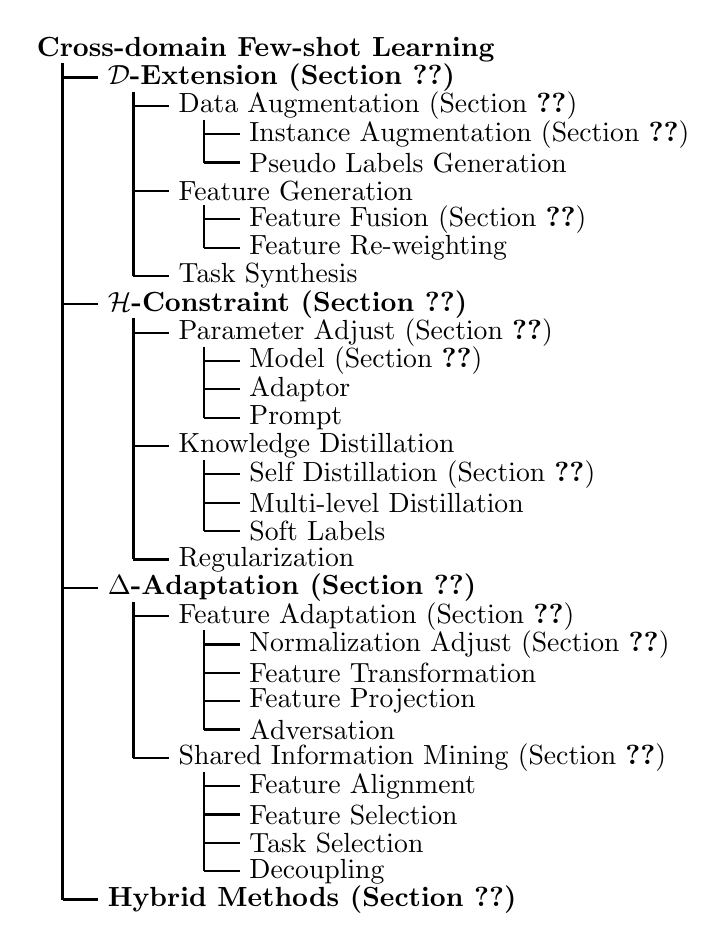
\begin{tikzpicture}[xscale=0.9, yscale=0.36]
\textcolor{black}{
\draw [thick, -] (0, 24) -- (0, 24); \node [right] at (-0.5, 24) {\textbf{Cross-domain Few-shot Learning
}};
\draw [thick, -] (0, 23.5) -- (0, -6);
\draw [thick, -] (0, 23) -- (0.5, 23);\node [right] at (0.5, 23) {\textbf{$\mathcal{D}$-Extension (Section~\ref{instance})}};
\draw [thick, -] (1, 22.5) -- (1, 16);
\draw [thick, -] (1, 22) -- (1.5, 22);\node [right] at (1.5, 22) {Data Augmentation (Section~\ref{sec:FSCIC:dba})};
\draw [thick, -] (2, 21.5) -- (2,20);
\draw [thick, -] (2, 21) -- (2.5, 21);\node [right] at (2.5, 21) {Instance Augmentation (Section~\ref{sec:FSCIC:dba:drbm})};
%\draw [thick, -] (2, 20.5) -- (2,19);
\draw [thick, -] (2, 20) -- (2.5, 20);\node [right] at (2.5, 20) {Pseudo Labels Generation};
\draw [thick, -] (1, 19) -- (1.5, 19);\node [right] at (1.5, 19) {Feature Generation
};
\draw [thick, -] (2, 18.5) -- (2,17);
\draw [thick, -] (2, 18) -- (2.5, 18);\node [right] at (2.5, 18) {Feature Fusion (Section~\ref{sec:FSCIC:dba:drbm})};
%\draw [thick, -] (2, 20.5) -- (2,19);
\draw [thick, -] (2, 17) -- (2.5, 17);\node [right] at (2.5, 17) {Feature Re-weighting};
\draw [thick, -] (1, 16) -- (1.5, 16);\node [right] at (1.5, 16) {Task Synthesis
};
\draw [thick, -] (0, 15) -- (0.5, 15);\node [right] at (0.5, 15) {\textbf{$\mathcal{H}$-Constraint (Section~\ref{hypothesis})}};
\draw [thick, -] (1, 14.5) -- (1, 6);
\draw [thick, -] (1, 14) -- (1.5, 14);\node [right] at (1.5, 14) {Parameter Adjust (Section~\ref{sec:FSCIC:dba})};
\draw [thick, -] (2, 13.5) -- (2,11);
\draw [thick, -] (2, 13) -- (2.5, 13);\node [right] at (2.5, 13) {Model (Section~\ref{sec:FSCIC:dba:drbm})};
%\draw [thick, -] (2, 20.5) -- (2,19);
\draw [thick, -] (2, 12) -- (2.5, 12);\node [right] at (2.5, 12) {Adaptor};
\draw [thick, -] (2, 11) -- (2.5, 11);\node [right] at (2.5, 11) {Prompt};
\draw [thick, -] (1, 10) -- (1.5, 10);\node [right] at (1.5, 10) {Knowledge Distillation
};
\draw [thick, -] (2, 9.5) -- (2,7);
\draw [thick, -] (2,9) -- (2.5, 9);\node [right] at (2.5, 9) {Self Distillation (Section~\ref{sec:FSCIC:dba:drbm})};
%\draw [thick, -] (2, 20.5) -- (2,19);
\draw [thick, -] (2, 8) -- (2.5, 8);\node [right] at (2.5, 8) {Multi-level Distillation};
\draw [thick, -] (2, 7) -- (2.5, 7);\node [right] at (2.5, 7) {Soft Labels};
\draw [thick, -] (1, 6) -- (1.5, 6);\node [right] at (1.5, 6) {Regularization
};
\draw [thick, -] (0, 5) -- (0.5, 5);\node [right] at (0.5, 5) {\textbf{$\Delta$-Adaptation (Section~\ref{adaptation})}};
\draw [thick, -] (1, 4.5) -- (1, -1);
\draw [thick, -] (1, 4) -- (1.5, 4);\node [right] at (1.5, 4) {Feature Adaptation (Section~\ref{sec:FSCIC:dba})};
\draw [thick, -] (2, 3.5) -- (2,0);
\draw [thick, -] (2, 3) -- (2.5, 3);\node [right] at (2.5, 3) {Normalization Adjust (Section~\ref{sec:FSCIC:dba:drbm})};
%\draw [thick, -] (2, 20.5) -- (2,19);
\draw [thick, -] (2, 2) -- (2.5, 2);\node [right] at (2.5, 2) {Feature Transformation};
\draw [thick, -] (2, 1) -- (2.5, 1);\node [right] at (2.5, 1) {Feature Projection};
\draw [thick, -] (2, 0) -- (2.5, 0);\node [right] at (2.5, 0) {Adversation
};
%\draw [thick, -] (2, -0.5) -- (2,-2);
\draw [thick, -] (1,-1) -- (1.5, -1);\node [right] at (1.5, -1) {Shared Information Mining (Section~\ref{sec:FSCIC:dba:drbm})};
\draw [thick, -] (2, -1.5) -- (2,-5);
\draw [thick, -] (2, -2) -- (2.5, -2);\node [right] at (2.5, -2) {Feature Alignment};
\draw [thick, -] (2, -3) -- (2.5, -3);\node [right] at (2.5, -3) {Feature Selection};
\draw [thick, -] (2, -4) -- (2.5, -4);\node [right] at (2.5, -4) {Task Selection};
\draw [thick, -] (2, -5) -- (2.5, -5);\node [right] at (2.5, -5) {Decoupling};
\draw [thick, -] (0, -6) -- (0.5, -6);\node [right] at (0.5, -6) {\textbf{Hybrid Methods (Section~\ref{hybrid})}};}
\end{tikzpicture}}
\vspace{-10pt}
\caption{\textcolor{black}{The taxonomy of representative methods in CDFSL.}}
\label{out}
\end{figure}
%\end{wrapfigure}
\fi
% \section{Datasets and benchmarks}\label{evaluation}
This section exhibits the evaluation tools for CDFSL models, the datasets used in CDFSL task are described in Section~\ref{data}, Section~\ref{benchmark} collects the existing benchmarks utilized for CDFSL problem. And we summarize in Section~\ref{sum}.

\subsection{Datasets} \label{data}
Annotated datasets are used to provide a fair comparison among diferent algorithms and architectures. Furthermore, the growth in complexity, size, annotation number, and transfer difficult of datasets increases the challenge level, encouraging in constant development of new and improved techniques. The most used datasets for the CDFSL task as follows: 
\begin{itemize}
    \item \textit{mini}ImageNet\cite{miniimagenet}: \textit{mini}ImageNet dataset is composed of 60000 images selected from the dataset ImageNet, with a total of 100 categories. Each category has 600 images, and the size of each image is $84 \times 84$.
    
    \item \textit{tiered}ImageNet\cite{tieredimagenet}: This dataset is selected from the ImageNet dataset, including 34 categories, each category contains 10-30 sub-categories (classes). There are 608 classes and 779165 images in this dataset, each class has multiple samples of varying numbers.
    
    \item Plantae\cite{plantae}: Plantae dataset is one of dataset iNat2017. There are 2101 categories and 196613 images in this dataset.
    \item Places\cite{places}: Places dataset contains more 10 million images comparising 400+ unique scene categories. This dataset features 5000 to 30000 training images in each class, consistent with real-world frequencies of occurrence. The image size in this dataset is $200 \times 200$.
    \item Stanford Dogs\cite{dogs}: The Stanford Dogs dataset contains over 20,000 images of 120 breeds of dogs from around the world. This dataset has been built using images and annotation from ImageNet for the task of fine-grained image categorization. It was originally collected for fine-grain image categorization, a challenging problem as certain dog breeds have near identical features or differ in colour and age..
    \item Stanford Cars\cite{cars}: The Cars dataset is a fine-grained classification dataset about cars. It contains 16,185 images of 196 classes of cars. The data is split into 8,144 training images and 8,041 testing images.
    \item CUB\cite{cub}: Images in CUB dataset overlap with images in ImageNet. It is a fine-grained classification dataset about birds that contain 11788 images in 200 categories. The size of images in this dataset is $84 \times 84$.
    \item CropDiseases\cite{cropdiseases}: CropDiseases dataset consists of about 87000 RGB images of healthy and diseased crop leaves which is categorized into 38 different classes. The total dataset is divided into 80/20 ratio of training and validation set. The image size in this dataset is $256 \times 256$.
    \item EuroSAT\cite{eurosat}: EuroSAT is a dataset for land use and land cover classification. The dataset is based on Sentinel-2 satellite images covering 13 spectral bands and consisting out of 10 classes with in total 27,000 labeled and geo-referenced images. Each class includes 2000-3000 images, the size of these images is $64 \times 64$.
    \item ISIC 2018\cite{isic1}\cite{isic2}: ISIC 2018 dataset includes 10015 dermoscopic lesion images from 7 categories for training, 193 images for evaluate, and 1512 images for testing. The size of each image is $600 \times 450$.
    \item ChestX\cite{chestx}: ChestX-ray14 is currently the largest lung X-ray database provided by the NIH Research Institute, which contains 14 lung diseases (atelectasis, consolidation, infiltration, pneumothorax, edema, emphysema, fibrosis, More than 100,000 X-ray front views of fluid, pneumonia, pleural thickening, cardiac hypertrophy, nodules, masses, and hernias), categories 1-14 correspond to 14 lung diseases, and category 15 indicates no disease was found. The size of images in this dataset is $1024 \times 1024$.
    \item Omniglot\cite{omniglot}: The Omniglot dataset is composed of 1,623 handwritten characters from 50 different languages, each with 20 different handwritings, which constitutes an dataset that contains extremely large number of sample categories (1623), but a very small sample number (20) of samples in each category. The size of each image in this dataset is $28 \times 28$.
    \item CIFAR-FS\cite{cifar}: The full name of the CIFAR-FS dataset is the CIFAR100 Few-Shots dataset, which is derived from the CIFAR 100 dataset and contains 100 categories, with 600 images in each category, for a total of 60,000 images. In use, it is usually divided into training set (64 types), validation set (16 types) and test set (20 types), and the image size is unified to $32 \times 32$.
    \item FGVC-Aircraft\cite{aircraft}: FGVC-Aircraft dataset includes 10200 aircraft images (102 aircraft models, 100 images per model). The image resolution is about 1-2 Mpixels.
    \item Describable Textures (DTD)\cite{dtd}: DTD is a texture database, consisting of 5640 images, organized according to a list of 47 terms (categories) inspired from human perception. There are 120 images for each category. Image sizes range between 300x300 and 640x640, and the images contain at least 90% of the surface representing the category attribute.
    \item Quick Draw\cite{draw1}: The Quick Draw Dataset is a collection of 50 million drawings across 345 categories, contributed by players of the game Quick, Draw!
    \item Fungi\cite{fungi}: This datasets contains 100000 fungi images belong to 1394 different categories, which is all fungi classes that have been spotted by the general public in Denmark.
    \item VGG Flower\cite{vgg}: VGG Flower dataset contains 8189 flower images belong to 102 categories. The flowers chosen to be flower commonly occuring in the United Kingdom. Each class consists of between 40 and 258 images.
    \item Traffic Signs\cite{traffic}: Traffic Signs dataset consists of 50,000 images of German road signs in 43 classes.
    \item MSCOCO\cite{mscoco}: The images in MSCOCO dataset are collected from Flickr with 1.5 million object instances belonging to 80 classes labelled and localized using bounding boxes.
\end{itemize}

\begin{table}
\tiny
\centering
\caption{Related datasets.}
\begin{tabular}{|c|c|c|c|c|c|c|c|c|}
\hline
Datasets & Derived from & \makecell[c]{Number of \\ images} & Image size & \makecell[c]{Number of \\ categories} & Content & Fields & Reference     \\ 
 \hline
\textit{mini}ImageNet & ImageNet & 60000 & $84 \times 84$ & 100 & objects classification & natural scene & \cite{miniimagenet}    \\  
\hline
\textit{tiered}ImageNet & ImageNet & 779165 & $84 \times 84$ & 608 & objects classification & natural scene & \cite{tieredimagenet}     \\
\hline
Plantae  & iNat2017 & 196613 & varying & 2101 & plants \& animals classification & natural scene & \cite{plantae}  \\
\hline
Places     & N/A & 10 million & $200 \times 200$ & 400+ & scene classification  & natural scene & \cite{places}   \\
\hline
Stanford Dogs     & ImageNet & 20000+ & varying & 120 & dogs fine-grained classification & natural scene &  \cite{dogs}   \\
\hline
Stanford Cars     & N/A & 16185 & varying & 196 & cars fine-grained classification & natural scene &  \cite{cars}   \\
\hline
CUB   & ImageNet & 11788 & $84 \times 84$ & 200 & birds fine-grained classification & natural scene &  \cite{cub}   \\  
\hline
CropDiseases   & N/A & 87000 & $256 \times 256$ & 38 & crop leaves classification & natural scene &  \cite{cropdiseases}  \\
 \hline
EuroSAT   & Sentinel-2 satellite & 27000 & $64 \times 64$ & 10 & land classification & remote sensing &  \cite{eurosat}   \\
\hline
ISIC 2018   & N/A & 11720 & $600 \times 450$ & 7 & dermoscopic lesion classification & medical &  \cite{isic1}   \\
\hline
ChestX   & N/A & 100K & $1024 \times 1024$ & 15 & lung diseases classification & medical & \cite{chestx}  \\
\hline
Omniglot   & N/A & 25260 & $28 \times 28$ & 1623 & characters classification & character &  \cite{omniglot}   \\
\hline
CIFAR-FS   & CIFAR 100 & 60000 & $32 \times 32$ & 100 & objects classification & natural scene &  \cite{cifar}   \\
 \hline
 
FGVC-Aircraft   & N/A & 10200 & varying & 100 & Aircraft fine-grained classification & natural scene &  \cite{aircraft}   \\
\hline

DTD   & N/A & 5640 & varying & 47 & textures classification & natural scene &  \cite{dtd}   \\
\hline
Quick Draw   & Quick draw! & 50 million & $128 \times 128$ & 345 & drawing images classification & Art &  \cite{draw1}   \\
\hline

Fungi   & N/A & 100000 & varying & 1394 & fungi fine-grained classification & natural scene &  \cite{fungi}   \\
\hline

VGG Flower   & N/A & 8189 & varying & 102 & flowers fine-grained classification & natural scene &  \cite{vgg}   \\
\hline

Traffic Signs   & N/A & 50000 & varying & 43 & Traffic signs classification & natural scene &  \cite{traffic}   \\
\hline

MSCOCO   & N/A & 1.5 million & varying & 80 & objects classification & natural scene &  \cite{mscoco}   \\
\hline
\end{tabular}
\end{table}

\subsection{Benchmarks} \label{benchmark}
This section mainly introduces the benchmarks of CDFSL problem, including \textit{miniImageNet \& CUB} (\textit{mini-CUB}), \textit{Meta-Dataset}, a standard fine-gained classification benchmark \textit{(FGCB)}, \textit{BSCD-FSL}.

\textbf{mini-CUB}.
In the early stage of CDFSL development, researchers usually use \textit{mini-CUB} to verify the performance of the proposed CDFSL algorithm. The images in \textit{mini}Imagenet~\cite{miniimagenet} are all natural images, and \textit{CUB}~\cite{cub} is a fine-grained image dataset about birds. Therefore, as one of the most commonly used benchmarks, it aims to verify the fine-grain based cross-domain performance of the CDFSL algorithm.

\textbf{DomainNet}~\cite{domainnet}
DomainNet is originally proposed to address UDA problem. Some approaches utilize it to evaluate the CDFSL performance. It contains 6 domains, with each domain containing 345 categories of common objects. The domains include Clipart, Infograph, Painting, Quickdraw, Real, and Sketch.

\textbf{Office-Home}~\cite{officehome}
Office-Home is a benchmark dataset for domain adaptation which contains 4 domains where each domain consists of 65 categories. The four domains are: Art, Clipart, Product, and Real-World. It contains 15,500 images, with an average of around 70 images per class and a maximum of 99 images in a class.

\textbf{Meta-Dataset}~\cite{meta-dataset}.
Meta-Dataset is a large-scale diverse benchmark, for measuring various image classification models in realistic and challenging few-shot contexts such as CDFSL. This dataset consists of 10 publicly available natural image datasets, handwritten characters, and graffiti datasets, including ILSVRC-2012 \cite{imagenet}, Omniglot \cite{omniglot}, Aircraft \cite{aircraft}, CUB-200-2011 \cite{cub}, Describable Textures \cite{dtd}, Quick Draw \cite{draw1}, Fungi \cite{fungi}, VGG Flower \cite{vgg}, Traffic Signs \cite{traffic} and MSCOCO \cite{mscoco}. These datasets were chosen because they are free and easy to obtain, span a variety of visual concepts (natural and human-made) and vary in how fine-grained the class definition is. %Figure \ref{meta-dataset} is a visual display of Meta-Dataset.

\textbf{FGCB}.
In the early stage of CDFSL development, researchers focused on fine-grain based cross-domain, so a conventional benchmark was derived: fine-grained benchmark. It contains five datasets such as \textit{mini}ImageNet, Plantae~\cite{plantae}, Places~\cite{places}, Cars~\cite{cars}, and CUB~\cite{cub}. \textit{mini}ImageNet is regard as source domain and other datasets as target domain. All images in the five datasets are natural images. The source domain include 60000 common objects, and the target domains are usually the fine-grained classification dataset, such as the images of Plantae, Cars, CUB are plants and animals, cars, and birds, respectively. This means that for this benchmark, the main challenge of across domains comes is how to transfer the category information from coarse to fine. %The visual display is shown in Figure\ref{fine-grained}.

\textbf{BSCD-FSL}~\cite{bscd-fsl}.
As a more challenging benchmrak in CDFSL, BSCD-FSL includes five datasets consists of  \textit{mini}ImageNet, CropDisease~\cite{cropdiseases}, EuroSAT~\cite{eurosat}, ISIC~\cite{isic1,isic2}, ChestX~\cite{chestx}. CropDisease is a fine-grained datasets of crop leaves, all images in which are industrial natural images. EuroSAT, ISIC, and ChestX have the different imaging ways with natural image, they are satellite images, dermatology images, and radiology images, respectively.

\begin{table}
\tiny
\centering
\caption{Related benchmarks.}
\begin{tabular}{|c|c|c|c|c|c|c|c|}
\hline
Benchmarks & Number of datasets & Source domain & Target domain & Related fields & Reference   \\ 
 \hline
mini-CUB & 2 & \textit{mini}ImageNet & CUB & natural scene & N/A   \\  
\hline
DomainNet & 6 & \textit{mini}ImageNet & \makecell[c]{ Clipart \& Infograph \& Painting \& Quickdraw \& Real \& \\ Sketch } & \makecell[c]{natural scene \\ art} & \cite{domainnet}   \\  
\hline
Office-Home & 4 & Real-World & \makecell[c]{ Art \& Clipart \& Product} & \makecell[c]{natural scene \\ art} & \cite{officehome}   \\  
\hline
Meta-Dataset & 10 & ILSVRC-2012 & \makecell[c]{ Aircraft \& CUB \& DTD \& Fungi \& VGGFlower \& \\ Traffic signs \& MSCOCO \& Omniglot \& Quick draw } & \makecell[c]{natural scene \\ character \\ art} & \cite{meta-dataset}       \\
\hline
FGCB & 5 & \textit{mini}ImageNet & \makecell[c]{Plantae \& Places \& Cars \& CUB } & natural scene &  N/A   \\
\hline
BSCD-FSL & 5 & \textit{mini}ImageNet & \makecell[c]{CropDisease \& EuroSAT \& ISIC \& ChestX } & \makecell[c]{natural scene \\ remote sensing \\ medical} & \cite{bscd-fsl}    \\
\hline
\end{tabular}
\end{table}
% \subsection{Metrics} \label{Sec:Protect_before}

% \subsection{Show Your Evidence} \label{Sec:Protect_Evidence}

\subsection{Summary} \label{sum}
In this section, we introduce the 20 datasets and 6 benchmarks that are commonly used in CDFSL. The currently proposed CDFSL algorithms can be divided into three taxonomies based on these datasets and benchmarks, which will be discussed in next section.
\section{Approaches} \label{methods}
% 在这里描述cdfsl标准的执行过程
% CDFSL offers a unified solution to both cross-domain and FSL problems. \textcolor{black}{Algorithm \ref{alg:baseline} outlines the CDFSL baseline process (contents without colorful boxes), consisting of two key steps: (1) Training a feature extractor on the source domain, and (2) Performing FSL on the target domain. The first step provides prior knowledge from the source domain, optimized via transfer learning~\cite{tfsurvey}, meta-learning~\cite{hospedales2021meta}, and metric learning~\cite{kaya2019deep} techniques. The second step focuses on learning the feature extractor and target classifier with limited supervision.} Based on the unique challenges, we categorize CDFSL algorithms into four types: \textcolor{black}{$\mathcal{D}$-Extension, $\mathcal{H}$-Constraint, $\Delta$-Adaptation, and Hybrid Methods. In Algorithm \ref{alg:baseline}, the key steps of $\mathcal{D}$-Extension, $\mathcal{H}$-Constraint, and $\Delta$-Adaptation are highlighted with red, green, and blue boxes, respectively.}
CDFSL offers a unified solution to both cross-domain and FSL problems. \textcolor{black}{Figure \ref{overview} outlines the CDFSL baseline process, consisting of two key steps: (1) Training a feature extractor on the source domain, and (2) Performing FSL on the target domain. The first step provides prior knowledge from the source domain, optimized via transfer learning~\cite{tfsurvey}, meta-learning~\cite{hospedales2021meta}, and metric learning~\cite{kaya2019deep} \etc techniques. The second step focuses on learning the feature extractor and target classifier with limited supervision.} Based on the unique challenges, we categorize CDFSL algorithms into four types: \textcolor{black}{$\mathcal{D}$-Extension, $\mathcal{H}$-Constraint, $\Delta$-Adaptation, and Hybrid Methods.}
% Specifically, the feature extractor and the source classifier are optimized through many labeled source data. The optimization in this step can be achieved by transfer learning, meta-learning, and metric learning technologies, \etc. While in the second step, following the vanilla few-shot learning setting, the final accuracy is obtained by calculating the average accuracy of multiple episodes. In each episodes, the support set and query set are first selected from the target data. The support set includes $C \times K$ samples, where $C$ means the number of classes and $K$ illustrates the samples in each category. And all the samples in query set are from the rest examples in $C$ categories. Then, the feature extractor and the target classifier are finetuned through the support set.


 % Based on the analysis of unique issue and challenges, \textcolor{black}{we present a classification criterion for CDFSL algorithms, dividing them into four categories: $\mathcal{D}$-Extension, $\mathcal{H}$-Constraint, $\Delta$-Adaptation, and Hybrid Methods.} % The overview of CDFSL is depicted in Figure~\ref{overview} (a).
 \iffalse
\begin{algorithm}
\caption{\textcolor{black}{Cross-domain Few-shot Learning (CDFSL) Baseline}}
\label{alg:baseline}
\begin{algorithmic} 
    \State \textbf{Input:} Source domain data $\mathcal{D}^{s}$ (with many labeled examples), Target domain data $\mathcal{D}^{t}$ (with few labeled examples), Initialized feature extractor $f$, Source classifier $\phi_{s}$, Target classifier $\phi_{t}$

    \State \textbf{Output:} Optimized feature extractor $f$ and target classifier $\phi_{t}$
    
    \State \textbf{Step 1: Train feature extractor on source domain}
    \State \fcolorbox{red}{white}{Augment $\mathcal{D}^{s}$}
    \State {\textbf{While} \textit{max epochs not reached} \textbf{do}}
    \State {\hspace{0.5cm} \textbf{for} each mini-batch \{$x_i$,$y_i$\} in $\mathcal{D}^{s}$ \textbf{do}} %\textcolor{red}{\Comment{$\mathcal{D}$-Extension: Augment and extend $\mathcal{D}^{s}$}}
    \State {\hspace{1.0cm} Input $x_i$ into $f$ to get the source features $\textbf{f}_i \gets f(x_i)$ 
    } %\newline \textcolor{green}{\Comment{$\mathcal{H}$-Constraint: Constrain hypothesis space $\mathcal{H}$ with strategies}}
    \State {\hspace{1.0cm} \fcolorbox{red}{white}{Augment $\textbf{f}_i$ } \fcolorbox{green}{white}{Constrain $f(\cdot)$ } \fcolorbox{blue}{white}{Adapt $\textbf{f}_i$ and $\textbf{f}_s$}}
    \State {\hspace{1.0cm} Input $\textbf{f}_{i}$ into $\phi_{s}$ to get the source predictions $\textbf{p}_i \gets \phi_{s}(\textbf{f}_{i})$ 
    }
    \State {\hspace{1.0cm} Compute the loss function between $\textbf{p}_i$ and $y_{i}$, update $f$ and $\phi_{s}$ 
    }  %\textcolor{black}{\Comment{$\Delta$-Adaptation: Adapt the distributions}}
    \State {\hspace{1.0cm} \fcolorbox{green}{white}{Constrain $\phi_{s} \circ f(\cdot)$ }}
    \State Test on the test data from the source domain, and get the pre-trained $f_{pre}$ 

    \State \textbf{Step 2: Few-shot learning on target domain}
    \State {\textbf{While} \textit{max episodes not reached} \textbf{do}}
    \State {\hspace{0.5cm} Randomly select $C$ categories and $K$ samples in each category ($C$-way $K$-shot) from $\mathcal{D}^{t}$} 
    \State {\hspace{0.5cm} Form the support set $(\mathcal{X}_s,\mathcal{Y}_s)$ with these $C \times K$ samples%, $\mathcal{X}_s$ and $\mathcal{Y}_s$ represent sample and label set in support set 
    }  %\textcolor{red}{\Comment{$\mathcal{D}$-Extension: Augment and extend $(\mathcal{X}_s,\mathcal{Y}_s)$}}
    \State {\hspace{0.5cm} \fcolorbox{red}{white}{Augment $(\mathcal{X}_s,\mathcal{Y}_s)$}}
    \State {\hspace{0.5cm} \textbf{While} \textit{max epochs not reached} \textbf{do}}
    \State {\hspace{1.0cm} Input $\{x_s,y_s\} \in (\mathcal{X}_s,\mathcal{Y}_s)$ into the pre-trained $f_{pre}$ (from step 1) to get $\textbf{f}_s \gets f_{pre}(x_s)$ } % \newline  \textcolor{green}{\Comment{Constrain hypothesis space $\mathcal{H}$ with strategies}}
    \State {\hspace{1.0cm} \fcolorbox{red}{white}{Augment $\textbf{f}_s$ } \fcolorbox{green}{white}{Constrain $f_{pre}(\cdot)$ } \fcolorbox{blue}{white}{Adapt $\textbf{f}_s$ to $\textbf{f}_i$}}
    \State {\hspace{1.0cm} Input $\textbf{f}_s$ into the initialized $\phi_{t}$ to get the target predictions $\textbf{p}_s \gets \phi_{t}(\textbf{f}_{s})$ }
    \State {\hspace{1.0cm} \fcolorbox{blue}{white}{Adapt $\textbf{p}_s$ to $\textbf{p}_i$}}
    \State {\hspace{1.0cm} Compute the loss function between $\textbf{p}_s$ and $y_{s}$, update $f_{pre}$ and $\phi_{t}$}
    \State {\hspace{1.0cm} \fcolorbox{green}{white}{Constrain $\phi_{t} \circ f_{pre}(\cdot)$ }}

    \State {\hspace{0.5cm} Randomly select the rest samples from the same $C$ categories with $(\mathcal{X}_s,\mathcal{Y}_s)$ as query set $\mathcal{X}_{q}$ }
    \State {\hspace{0.5cm} Input $x_q \in \mathcal{X}_q$ into the updated $f_{pre}$ and $\phi_{t}$ to get the $\textbf{p}_q \gets \phi_{t} \circ f_{pre} (x_q)$ }
    \State {\hspace{0.5cm} Compute the accuracy with $\textbf{p}_q$ }

    \State Calculate the mean accuracy of all the episodes
\end{algorithmic}
\end{algorithm}
\vspace{-0.3cm}
\fi


\begin{figure}%[h]
	\centering
	\includegraphics[width=11cm]{response/crop_overview1.pdf}
  \vspace{-0.3cm}
	\caption{\textcolor{black}{An overview of the CDFSL method involves two main stages. First, existing techniques pretrain the encoder on the source domain. Second, the encoder is finetuned, and a target recognizer is trained on the support set (with limited labeled data) of target domain. And inference is performed using the finetuned encoder and the target recognizer on the query set. $\textit{D}^{s}$ and $\textit{D}^{t}$ mean the source and target data.}}
  \vspace{-0.3cm}
	\label{overview}
\end{figure}


\textcolor{black}{
\subsection{$\mathcal{D}$-Extension}  \label{instance}
\textcolor{black}{$\mathcal{D}$-Extension enhances and expands existing information resources to improve the model’s generalization to new tasks, addressing the issue of unreliable TSERM. In CDFSL, information is typically represented in three dimensions: data space, feature space, and task space. Based on the dimension of information expansion, methods are classified into data augmentation, feature generation, and task synthesis. This classification demonstrates how $\mathcal{D}$-Extension systematically addresses the challenge of information scarcity across these three dimensions. Figure~\ref{fig_instance} illustrates how these methods work.}
% \textcolor{black}{$\mathcal{D}$-Extension enhances and expands existing information resources to improve the model’s ability to generalize to new tasks. It is not limited to simple data generation but spans multiple aspects, aiming to maximize the use of available resources. By focusing on different aspects, $\mathcal{D}$-Extension can be divided into three main subcategories: data augmentation, feature generation, and task synthesis. This classification systematically demonstrates how $\mathcal{D}$-Extension addresses the challenge of information scarcity across the dimensions of data, features, and tasks. It not only helps researchers and practitioners better understand and select appropriate augmentation strategies but also clarifies the specific role each method plays in enhancing model performance. Figure~\ref{fig_instance} and Table~\ref{table_instance} indicate the details of these methods.}
% This section presents approaches that extend the information of $\mathcal{D}$, including the source domain $\mathcal{D}^{s}$ and target domain $\mathcal{D}^{t}$, to improve the performance of CDFSL. Existing methods are divided into data augmentation, feature generation, and task synthesis according to the different aspects of information expansion. Specifically, data augmentation expands information at the data level, including instance augmentation and pseudo-label generation. While feature generation aims to generate new and effective features through strategies such as feature fusion or feature re-weighting. These features can fill in the gaps that the original information cannot cover, and by processing features at different levels, a more target task-friendly representation can be obtained. Furthermore, some other methods enhance the generalization ability of the model by constructing diverse tasks, especially difficult tasks. It should be noted that although task synthesis needs to be performed on the basis of data augmentation, its core idea is to increase the diversity and difficulty of tasks and thus improve the generalization of the model, rather than simply augmenting the data in a single task. These approaches are illustrated in Figure~\ref{fig_instance}, and their details are presented in Table~\ref{table_instance}.
}
\begin{figure}%[h]
	\centering
	\includegraphics[width=\linewidth]{response/crop_extension1.pdf}
  \vspace{-0.5cm}
	\caption{\textcolor{black}{Solving CDFSL problem by $\mathcal{D}$-Extension, including data augmentation, feature generation, and task synthesis. Data augmentation aims to augment data by instance/pseudo-label generation, \etc. Feature generation enhances the features by fusing or re-weighting them. And task synthesis improves model generalization by generating more guided tasks. The core operations of methods are highlighted in red. % We classify existing CDFSL methods into \textcolor{black}{$\mathcal{D}$-Extension, $\mathcal{H}$-Constraint, $\Delta$-Adaptation, and Hybrid Methods.
    }}
  \vspace{-0.3cm}
	\label{fig_instance}
\end{figure}

\iffalse
\begin{table}
\tiny
\centering
\caption{Representative $\mathcal{D}$-Extension approaches. `$FG$', `$Art$' and `$IW$' indicate that evaluation of Fine-grained CDFSL ($FG$), Art-based CDFSL ($Art$) and imaging way-based CDFSL ($IW$), respectively.}
\vspace{-0.2cm}
\setlength{\tabcolsep}{3.6mm}{
\begin{tabular}{llcccccc}
\hline
\textbf{Methods} & \textbf{Venue} & \textbf{Augment aspect} & \textbf{Augmented information from} & \textbf{Loss function} & \textbf{FG} & \textbf{Art} & \textbf{IW}      \\ 
 \hline
NSAE~\cite{boosting} & ICCV 2021 & Data Augmentation  & Instances & CE\& BSR & \Checkmark &  & \Checkmark \\
% \hline
TGDM~\cite{tgdm} & ACM MM 2022 & Data Augmentation  & Instances & CE & \Checkmark &  &  \\  
% \hline
ISSNet~\cite{data_multi_3}   & ICIP 2023 & Data Augmentation & Instances & BSR \& Perceptual \& Style &  &  & \Checkmark     \\
% \hline
SSA-BNS~\cite{sreenivas2023similar}  & CVPR 2023 & Data Augmentation & Instances & $L_{NCC}$ &  & \Checkmark &    \\
% \hline
CDPSN~\cite{data_other_1} & Scientific Reports 2023 & Data Augmentation  & Instances & CE &  &   & \Checkmark \\  
% \hline
FAP~\cite{extend_1} & arXiv 2024 & Data Augmentation  & Instances & CE \& KL &   \Checkmark    &   & \Checkmark \\  
% \hline
UD~\cite{data_target_2}   &  arXiv 2021 & Data Augmentation &  Pseudo Label & Contrastive &  & \Checkmark &    \\
% \hline
STARTUP~\cite{st} & ICLR 2021 & Data Augmentation & Pseudo Label & CE \& KL \& SimCLR &  &  & \Checkmark  \\
% \hline
CHEF~\cite{rf}   & arXiv 2020 & Feature Generation & Feature Fusion & CE &  &  & \Checkmark  \\
% \hline
PKTN~\cite{mdfsl}  & IJON 2021 & Feature Generation & Feature Fusion & Consistency &  \Checkmark   &  &    \\  
% \hline
RMP~\cite{feature_fusion_2} & ACM MM 2021 & Feature Generation & Feature Fusion & CE \& $L_{2}$ & \Checkmark  &  &   \\
% \hline
DFTL~\cite{parameter_fix_3} & ICAICA 2021 & Feature Generation & Feature Fusion & CE & \Checkmark &  &    \\
% \hline
GA-GNN~\cite{liu2022geometric} & APPL INTELL 2022 & Feature Generation & Feature Fusion & CE & \Checkmark &  &   \\
% \hline
RDC~\cite{feature_reweight_6} & CVPR 2022 & Feature Generation & Feature Fusion & CE \& KL & \Checkmark &  & \Checkmark  \\
% \hline
KT~\cite{li2023knowledge} & PR 2023 & Feature Generation & Feature Fusion & CE \& MSE &  &  & \Checkmark \\
%\hline
DeepEMD~\cite{feature_reweight_3} & ISCIPT 2021 & Feature Generation & Feature Re-weighting & CE & \Checkmark &  &    \\
% \hline
FUM~\cite{feature_reweight_7} & PR 2022 & Feature Generation & Feature Re-weighting & CE & \Checkmark & \Checkmark &   \\
% \hline
HVM~\cite{parameter_weight_2}  & ICLR 2022 & Feature Generation & Feature Re-weighting & ELBO &  &  & \Checkmark    \\  
% \hline
Wave-SAN~\cite{parameter_fix_9} & arXiv 2022 & Feature Generation & Feature Re-weighting & CE \& KL & \Checkmark  &  & \Checkmark  \\
% \hline
AFGR~\cite{parameter_weight_3} & NCA 2022 & Feature Generation & Feature Re-weighting & CE & \Checkmark &  &  \\
%\hline
AFA~\cite{adversarial} & ECCV 2022 & Feature Generation & Feature Re-weighting & CE \& $L_{2}$ \& Adversarial & \Checkmark &  & \Checkmark \\
%\hline
StyleAdv~\cite{feature_reweight_0} & CVPR 2023 & Feature Generation & Feature Re-weighting & CE & \Checkmark &   & \Checkmark   \\
% \hline
ReqNet~\cite{ji2024relevance}   & IJMIR 2024 & Feature Generation & Feature Re-weighting & CE \& MI \& InfoNCE \& KL & \Checkmark &  & \Checkmark  \\
% \hline
ATA~\cite{ata} & IJCAI 2021 & Task Synthes & - & CE & \Checkmark &  & \Checkmark  \\
% \hline
AGE~\cite{feature_fusion_3} & AAAI 2022 & Task Synthes & - & CE &  & \Checkmark &   \\
% \hline
ST~\cite{data_other_2} & KBS 2023 & Task Synthes & - & CE & \Checkmark &  & \Checkmark  \\
% \hline
RDProtoFusion~\cite{rao2024rdprotofusion} & IJON 2024 & Task Synthes & - & CE \& Contrastive & \Checkmark &  & \Checkmark   \\
\hline
\end{tabular}}
\vspace{-0.5cm}
\label{table_instance}
\end{table}
\fi

\iffalse
 \begin{wrapfigure}{l}{180pt}
	\centering
  \vspace{-0.2cm}
	\includegraphics[width=6cm]{cdfsl-data-1.pdf}
 \vspace{-0.3cm}
	\caption{\textcolor{black}{The different categories of instance-guided approaches. Instances are from different origins. $\theta$ means the recognizer.}}
 \vspace{-0.5cm}
	\label{fig_instance}
\end{wrapfigure}
\fi

\subsubsection{\textcolor{black}{Data Augmentation.}} \label{data_original}
\textcolor{black}{Data augmentation expands the information by generating additional samples. Current methods introduce various types of transformations for models to learn, such as flipping~\cite{shyam2017attentive}, scaling~\cite{lake2015human, zhang2018fine}, translation~\cite{benaim2018one, lake2015human}, cropping~\cite{zhang2018fine}, shearing~\cite{shyam2017attentive}, reflection~\cite{edwards2017towards}, and rotation~\cite{model32, miniimagenet}. However, it's impractical to account for all potential transformations manually. Thus, affine transformations alone cannot fully solve the CDFSL problem~\cite{shyam2017attentive, lake2015human}. Next, we explore more advanced data augmentation methods at the sample and label levels, including instance augmentation and pseudo-label generation.}
% There are some approaches involve \textcolor{black}{the use of affine transformations, synthetic new data, and pseudo labels, as shown in Figure~\ref{fig_instance}. Affine transformations include flipping~\cite{shyam2017attentive}, scaling~\cite{lake2015human, zhang2018fine}, translation~\cite{benaim2018one, lake2015human, model32, shyam2017attentive}, cropping~\cite{zhang2018fine}, shearing~\cite{shyam2017attentive}, reflection~\cite{edwards2017towards}, and rotation~\cite{model32, miniimagenet}, \etc. Currently, almost of all CDFSL methods augment the samples with affine transformation manner. Therefore, here we ignore this augment strategy.}


\textbf{Instance Augmentation.}
\textcolor{black}{Instance augmentation~\cite{data_multi_3,sreenivas2023similar,extend_1,data_other_1,adcd,boosting,tgdm} increases sample diversity by synthesizing new data. Techniques include style transfer~\cite{data_multi_3,sreenivas2023similar}, frequency domain transformation~\cite{extend_1,data_other_1}, and adversarial methods~\cite{adcd,boosting}.} For instance, \cite{data_multi_3} introduces unlabeled data from multiple domains into the original source domain, generating large amounts of data with different styles but the same content. \textcolor{black}{\cite{sreenivas2023similar} augments data by applying the style of semantically similar categories to each class.} Additionally, \cite{extend_1} enhances samples by processing high-frequency components of source images, allowing the network to mimic human visual perception by selecting different frequency cues in recognition tasks. Similarly, \cite{data_other_1} generates a sketch map from the original image to capture high-frequency information. \textcolor{black}{\cite{adcd} improves model robustness by generating adversarial instances, while \cite{tgdm} facilitates knowledge transfer by introducing an intermediate domain through mixing source and target domain images.} Furthermore,~\cite{boosting} performs adversarial training with noise data, enhancing model robustness.
% \textcolor{black}{Instance augmentation focuses on synthesizing data through the style transfer~\cite{data_multi_3,sreenivas2023similar}, frequency domain transform~\cite{extend_1}, and adversarial~\cite{adcd}, \etc.}~\cite{data_multi_3} introduces unlabeled data from multiple domains into the original source domain to transfer diverse styles, generating a large amount of data with different styles but the same content.\textcolor{black}{Besides, ~\cite{sreenivas2023similar} uses the style of semantically similar categories to augment the data of each category. Moreover,~\cite{extend_1} processes the high-frequency components of the source image to generate frequency-aware enhanced samples, allowing the network to simulate the visual perception of humans choosing different frequency cues when facing new recognition tasks. In~\cite{data_other_1}, the original image and its generated sketch map are processed separately by different branches of the network. Besides,~\cite{adcd} enhances model robustness by generating adversarial instances.~\cite{tgdm} introduces an intermediate domain generated by mixing images in the source and the target domain to help knowledge transfer.}~\cite{boosting} enhances model robustness by generating noisy data.

\textcolor{black}{
\textbf{Pseudo-label Generation.}
%Moreover, pseudo labels generation aims at introducing the unlabeled data and generating the pseudo labels for these data~\cite{data_target_2,st}. 
Pseudo-label generation involves leveraging unlabeled data by assigning pseudo labels to it~\cite{data_target_2,st}. One early approach~\cite{data_target_2} enhances unlabeled data by applying rotations and assigning the rotation degree as the pseudo labels, turning transformation tasks into supervised learning problems. Additionally,~\cite{st} introduces unlabeled target data during the pre-training stage, generating pseudo labels for these data through a pre-trained model. This unlabeled target data serves as supplementary information from the target domain, helping to enrich the model's understanding of the target domain without manual annotation.
% Pseudo-label generation aims at introducing the unlabeled data and generating the pseudo labels for these data~\cite{data_target_2,st}. An early work~\cite{data_target_2} introduces the unlabeled data, rotates them, and uses the rotation degree as their pseudo labels. Moreover,~\cite{st} introduces the unlabeled target data in the pre-training phase, and obtains the pseudo labels for them. These unlabeled target data is the extra information from the target domain.
}
% Some approaches involve the use of additional information from the original data, such as semantic and visual information, to enhance the performance of FSL tasks, as shown in Figure~\ref{data-original}. Among them, some works extract this extra information through reconstructed instances, as depicted in the green background area of the Figure~\ref{data-original}.  For example, in~\cite{lscdfsl}, a Triplet Autoencoder (TriAE) is utilized to learn a shared feature representation. It incorporates both source and target instances, and leverages semantic information as an intermediate bridge. In~\cite{boosting}, an autoencoder is used to reconstruct the input data, and the reconstructed data is then utilized as additional visual information to aid in the training process and learn the shared feature representation. And~\cite{hybrid_5} distills the knowledge of multiple tasks/domain-specific networks into a single network. This is achieved by aligning the representations of the single network with the task/domain-specific ones using small capacity adapters.
 %\vspace{-0.2cm}
 \iffalse
 \begin{wrapfigure}{r}{180pt} 
	\centering
	\includegraphics[width=6cm]{cdfsl-data1-43.pdf}
 \vspace{-0.2cm}
	\caption{\textcolor{black}{Instances from extra information of original data. The extra information can be from generation model (green area) or other modal like texts (blue part). Dotted lines indicate the process of additional information introduction.}}
	\label{data-original}
 \vspace{-0.3cm}
\end{wrapfigure}
\fi

%Meanwhile, other works directly add additional information to the model, as shown in the blue part of Figure~\ref{data-original}. For instance,~\cite{mdfsl} presents a model that integrates visual and semantic information to recognize target categories, and utilizes weight imprinting for future fine-tuning. Furthermore, in~\cite{data_other_1}, the original image and its corresponding sketch map are processed separately by different branches of the network. The features extracted from the original image are combined with the contour features extracted from the sketch map branch during training, thus improving the accuracy and generalization performance of the model. Moreover,~\cite{data_other_2} proposes a task-expansion-decomposition framework for CD-FSL called the self-taught (ST) approach, which alleviates the problem of non-target guidance by constructing task-oriented metric spaces.

\subsubsection{\textcolor{black}{Feature Generation}} \label{data_multiple}
% By utilizing instances from multiple domains, a model can learn a general shared representation with broad generalization ability. The Domain-Agnostic Meta Learning (DAML) algorithm, proposed in~\cite{data_multi_2}, adapts the model to novel classes in seen and unseen domains. In contrast,~\cite{data_multi_3} introduces unlabeled data from multiple domains into the original source domain to transfer diverse styles, making the model more adaptable to various domains and styles. Moreover, most methods combine multiple strategies together with the multiple-domain introduction strategy, as shown in Section~\ref{hybrid}.
\textcolor{black}{Feature generation, as shown in Figure~\ref{fig_instance}, creates new feature representations from existing ones, enriching the feature space and improving the model's ability to capture data patterns, especially in scenarios with limited data. The goal of generating new features is either to expand the total information content or to explore key features in greater depth. According to the focus of generating features, methods can be divided into two categories: (1) feature fusion~\cite{rf,feature_fusion_2,mdfsl,parameter_fix_3,feature_reweight_6}, aims to increase the total information content, and (2) feature re-weighting~\cite{parameter_weight_2,ji2024relevance,parameter_fix_9,feature_reweight_3,feature_reweight_7,parameter_weight_3,adversarial,feature_reweight_0}, which focuses on increasing the amount of critical information in the feature to optimize information usage.}
% \textcolor{black}{Besides directly augment data, the other manner to extend the information is generating the new features (as shown in Figure~\ref{fig_instance}), which is to the following two purposes: (1) Increase the overall amount of information, (2) Dig out more key information. Based on these two purposes, we divide methods as feature fusion~\cite{mdfsl,rf,feature_fusion_2,parameter_fix_3,liu2022geometric,li2023knowledge} and feature re-weighting~\cite{parameter_weight_2,ji2024relevance,parameter_fix_9,feature_reweight_3,feature_reweight_7,parameter_weight_3,adversarial}. Feature fusion combines features of different representations to enhance the amount of information, while feature re-weighting assigns different weights to features based on their importance to optimize the use of information. These fused and re-weighted features further augment the effective information in the existing features. }
% \textcolor{black}{Besides directly augment data, the other manner to extend the information of data is generating the new features (as shown in Figure~\ref{fig_instance}), including feature fusion~\cite{mdfsl,rf,feature_fusion_2,parameter_fix_3,liu2022geometric,li2023knowledge} and feature re-weighting~\cite{parameter_weight_2,ji2024relevance,parameter_fix_9,feature_reweight_3,feature_reweight_7,parameter_weight_3,adversarial}. Feature fusion combines features of different representations to form a new feature representation, while feature re-weighting assigns different weights to features based on their importance to adjust their impact in the model. These fused and re-weighted features further mine the effective information in the existing features, expanding the amount of effective information. }

\textbf{Feature Fusion.}
\textcolor{black}{
There are two main types of feature fusion methods~\cite{rf,feature_fusion_2,mdfsl,parameter_fix_3,feature_reweight_6} discussed here: multi-level fusion~\cite{rf,feature_fusion_2} and multi-model fusion~\cite{mdfsl,parameter_fix_3,feature_reweight_6}. Multi-level fusion focuses on combining features from different layers of the same model, addressing the limitations of using single-layer features. Low-level features may lack the specificity needed for complex tasks, while high-level features can overfit to the training data. By fusing these features, a more balanced and versatile representation is created, capable of handling a wide range of tasks~\cite{lin2017feature}. For example,\cite{rf} computes the loss for the last few layers of the model and sums them up as the final loss, while\cite{feature_fusion_2} fuses mid-level features to predict the residual term.}
% There are two ways to fuse the features, multi-level fusion~\cite{rf,feature_fusion_2} and multi-model fusion~\cite{mdfsl,parameter_fix_3,li2023knowledge,feature_reweight_0}, in the feature fusion. In which, multi-level fusion aims to fuse the features of different layers of the same model and mitigate the limitations of using single-layer features alone. Low-level features might lack the specificity needed for complex tasks, and high-level features might overfit to specific training data. The fusion of these features creates a more balanced and versatile feature representation, capable of handling a wide range of tasks and conditions effectively~\cite{lin2017feature}. Specifically,~\cite{rf} calculates the loss of the features of the last few layers of the model separately and sums them up as the final loss.~\cite{feature_fusion_2} introduces and fuses the mid-level features to predict the residual term.}
% There are two ways to fuse the features, multi-level fusion~\cite{rf,feature_fusion_2,liu2022geometric} and multi-model fusion~\cite{mdfsl,parameter_fix_3,li2023knowledge,feature_reweight_0}, in the feature fusion. In which, multi-level fusion aims to fuse the features of different layers of the same model and mitigate the limitations of using single-layer features alone. Low-level features might lack the specificity needed for complex tasks, and high-level features might overfit to specific training data. The fusion of these features creates a more balanced and versatile feature representation, capable of handling a wide range of tasks and conditions effectively~\cite{lin2017feature}. Specifically,~\cite{rf} calculates the loss of the features of the last few layers of the model separately and sums them up as the final loss. While~\cite{feature_fusion_2} introduces and fuses the mid-level features to predict the residual term. Moreover,~\cite{liu2022geometric} constructs a high-dimensional geometric algebra (GA) space in the non-Euclidean domain to help in reducing the distortion of feature information that typically increases with the depth of the network layers.

\textcolor{black}{
Multi-model fusion~\cite{mdfsl,parameter_fix_3,feature_reweight_6} refers to combining features generated by different models or strategies. Since these features come from diverse sources, fusing them leverages the strengths of each, creating a richer and more distinguishable feature representation. For instance,\cite{mdfsl} fuses knowledge from both class and semantic aspects,\cite{parameter_fix_3} averages the features from multiple models, and~\cite{feature_reweight_6} constructs a non-linear subspace, then combines the features from this subspace with the original features.
% While the multi-model fusion~\cite{mdfsl,parameter_fix_3,li2023knowledge} refers to the fusion of features generated by multiple different models or strategies. Since these features come from different models or strategies, when these features are fused together, they can give full play to their respective advantages and form a richer and more discernible feature representation.~\cite{mdfsl} fuse the knowledge from both class and semantic aspects.~\cite{parameter_fix_3} takes the average of the features from models with diversified feature transformation layers. And~\cite{li2023knowledge} introduces the information from query set. Besides, the features of the support set are combined in~\cite{li2023knowledge} with the query set features to calculate the loss. And~\cite{feature_reweight_6} uses a hyperbolic tangent transformation to construct a non-linear subspace, then combine the features from this subspace and the original feature.
}

\textbf{Feature Re-weighting.}
\textcolor{black}{
Feature re-weighting~\cite{parameter_weight_2,ji2024relevance,parameter_fix_9,feature_reweight_3,feature_reweight_7,parameter_weight_3,feature_reweight_0,adversarial} adjusts the weights of different features so the model can adaptively select the most important ones for different tasks or domains, improving performance.} For example, \cite{parameter_weight_2} learns separate weights for each multi-level feature, \cite{parameter_fix_9} re-weights features across different episodes, and~\cite{feature_reweight_7} introduces a forget-update module to re-weight features. Meanwhile, \cite{parameter_weight_3} applies attention mechanisms across multiple levels, \textcolor{black}{and \cite{ji2024relevance} re-weights both original and style-transformed features through context interaction. \cite{feature_reweight_3} enhances feature representation by leveraging local feature correlations, while \cite{feature_reweight_0} inputs style-altered features into the FSL classifier.~\cite{adversarial} explores adversarial feature augmentation to simulate distribution variations by re-weighting features.
% Feature re-weighting~\cite{parameter_weight_2,ji2024relevance,parameter_fix_9,feature_reweight_3,feature_reweight_7,parameter_weight_3,feature_reweight_0,adversarial} adjusts the weights of different features so that the model can adaptively select the most important features in different tasks or domains, thereby improving the performance of the model.} Among them,~\cite{parameter_weight_2} learns weights for each multi-level feature separately and re-weights them.~\cite{parameter_fix_9} explores a style augmentation module in each layer to re-weight the features between different episodes.~\cite{feature_reweight_7} explores a forget-update module to re-weight the feature in each layer.~\cite{parameter_weight_3} applies attention mechanisms at multiple levels to re-weight features to capture details at different scales. \textcolor{black}{Furthermore,~\cite{ji2024relevance} first transfers the style of the features, then interacts with the original and style-transformed features across context and re-weight them.~\cite{feature_reweight_3} enhance feature representation by leveraging the correlation between local features. In \cite{feature_reweight_0}, the style attacked features obtained through style transfer are input into the FSL classifier.~\cite{adversarial} explores a adversarial feature augmentation module to generates augmented features to simulate distribution variations by re-weight the features.
}



\vspace{-0.2cm}
\subsubsection{\textcolor{black}{Task Synthesis}} \label{data_target}
%Approaches that leverage target domain instances aim to uncover the shared information between the source and target domains. Some of these approaches employ a teacher-student network to aid
\iffalse
\begin{wrapfigure}{l}{150pt} 
	\centering
 \vspace{-0.4cm}
	\includegraphics[width=5cm]{cdfsl-data3.pdf}
 \vspace{-0.4cm}
	\caption{\textcolor{black}{STARTUP~\cite{st} structure. The dotted line represents how to use the auxiliary target data.}}
	\label{data-target}
 \vspace{-0.3cm}
\end{wrapfigure}
\fi
%training phase. CDFSL learning. For example, in~\cite{st}, (illustrated in Figure~\ref{data-target}), a self-training method is proposed that utilizes unlabeled target data to improve the source domain representation. It is the first work to introduce the unlabeled target data into the~\cite{dynamic} follows this setting and enforces consistency by comparing predictions of weakly-augmented unlabeled target data from a teacher network to strongly-augmented versions of the same images from a student network. Meanwhile,~\cite{data_target_2} develops a self-supervised learning approach to fully leverage unlabeled target domain data.
%(as depicted in the right part of Figure~\ref{data-target}).
%Other works integrate all labeled target data directly into the training process. For instance,~\cite{data_target_1} presents a Domain-Switch Learning (DSL) framework that embeds cross-domain scenarios into the training phase in a ``fast switching'' manner using multiple target domains.
\textcolor{black}{Task synthesis~\cite{ata,feature_fusion_3,rao2024rdprotofusion,data_other_2} (Figure~\ref{fig_instance}) expands the task space by creating new task scenarios or combinations, improving the model’s ability to generalize. Some methods generate challenging tasks to train the model in difficult situations. For example, \cite{ata} generates tasks simulating worst-case scenarios, helping the model adapt to a wider distribution of tasks during training. Other approaches synthesize tasks at the graph level. For instance, \cite{feature_fusion_3} augments task graphs into contextual and geometric views, while \cite{rao2024rdprotofusion} integrates information from different tasks using a multi-task learning framework. Additionally, \cite{data_other_2} randomly combines affine-transformed samples into diverse tasks.}
% \textcolor{black}{Task synthesis (Figure~\ref{fig_instance}) methods~\cite{ata, feature_fusion_3, rao2024rdprotofusion, data_other_2} aims to explore or synthesize diverse tasks to enhance the generalization of the model. Some of them synthesize challenging tasks to train the model's ability to handle difficult tasks. For example,~\cite{ata} generates challenging tasks that simulate worst-case scenarios, thus enabling the model to adapt to a wider distribution of tasks during training. Some other approaches synthesize the tasks at the graph level. For instance, the graphs from tasks in~\cite{feature_fusion_3} are augmented to a contextual view and two geometric view. Besides,~\cite{rao2024rdprotofusion} adopts a multi-task learning framework to integrate information from different tasks to improve the generalization ability and robustness of the model. And~\cite{data_other_2} randomly combines affine transformed samples into diverse tasks to improve model generalization.}

\subsubsection{Discussion and Summary}
% \textbf{Discussion and summary}
% 实验结果,结果分析,总结这类方法以及子类别方法的优缺点
% Instance-guided strategies are chosen based on the availability of data. When the source domain includes extra information such as semantic and visual information, utilizing instances from the original source (as described in Section~\ref{data_original}) is an effective approach. However, in scenarios where extra information is not available, introducing instances from the target domain (as discussed in Section~\ref{data_target}) could be a better option. In cases where target data is scarce or unavailable, utilizing instances from multiple domains (as outlined in Section~\ref{data_multiple}) can also be helpful.
% 每个子类别的优缺点
\textcolor{black}{
When additional unsupervised samples or data generation methods are available, the amount of information can be expanded through data augmentation. However, in data augmentation, particularly in instance augmentation, the augmented information is typically derived from the original samples, which results in limited valid information gain and a lack of real-world diversity. Additionally, the quality of generated pseudo-labels depends on the model's predictions; if the model has biases, the pseudo-label generation process may further amplify these biases.}

\textcolor{black}{When multiple features, including those from multiple models or levels, are available, feature generation methods can be applied. These methods enrich the feature space by processing multiple features to enhance the information. However, since these features come from the same examples, they are often highly correlated or redundant, which increases model complexity while providing limited additional information. Therefore, finding the optimal solution requires very fine adjustment~\cite{he2016deep}.}

\textcolor{black}{Finally, when auxiliary tasks are present, task synthesis enhances diversity by combining new tasks. However, this increased diversity can make the model’s learning objectives unclear and task relevance ambiguous. This occurs because different tasks may conflict or lack consistency, making it difficult for the model to identify which features or patterns are most important for the primary task. Additionally, auxiliary tasks can introduce irrelevant noise, further confusing the learning process. As a result, the composed tasks may not align well with the actual task, leading to sub-optimal performance in real-world applications~\cite{al32}.}
% $\mathcal{D}$-Extension methods improve the generalization ability of the model by expanding the amount of information. This is a very simple and easy method that can be directly applied to existing models. Specifically, data augmentation methods, including instance augmentation and pseudo-label generation, are effective methods when the sample generation mode is effective or unsupervised samples are available. It is the most intuitive method to expand information by increasing the amount of available data. Unlike data augmentation, which focuses on simply expanding the amount of data, task synthesis focuses more on the way of task composition. In addition, feature generation is feasible when multiple features are available or additional weights are available.

% \textcolor{black}{
% However, such methods still have some disadvantages, as they can introduce noise during the process of expanding information, which may ultimately mislead the learning of model. Specifically, data augmentation methods expand the information by introducing the augmented data, while it needs to ensure the accuracy of the generated samples or pseudo-labels, as inaccurate ones can introduce noise~\cite{inoue2018data}. Feature generation methods have different feature representations under the different combinations or weighting methods, and the optimal solution requires very fine adjustment~\cite{he2016deep}. In addition, the quality of the synthesis task is affected by the synthesis way, \ie improper task synthesis may cause task bias, which in turn leads to model training bias~\cite{al32}. }

% \textcolor{black}{However, such methods still have some disadvantages. Specifically, in data augmentation, especially in instance augmentation, the augmented information is usually from the original samples, resulting in a limited valid information gain and a lack of real-world diversity. Besides, the quality of generated pseudo-labels depends on the model's predictions. If the model has biases, the pseudo-label generation process may further amplify these biases. Task synthesis enhances diversity by composing new tasks, while these diversity tasks may results in a fuzzy model learning objectives and the unclear task relevance, \ie the synthetic tasks may not be completely relevant to the actual tasks, resulting in poor performance of the model in real applications~\cite{al32}. Recently,~\cite{data_multi_3} augments the data under the guidance of the style of the target domain, which increases the diversity of the data while also improving the relevance of the data to the task. In addition, in feature generation, choosing which features to generate and retain requires experience and domain knowledge, which is difficult. An unreasonable generated feature may be highly correlated or redundant with the original feature, which increases the complexity of the model without bringing additional information. Therefore, the optimal solution requires very fine adjustment~\cite{he2016deep}.}
% \textcolor{black}{However, such methods still have some disadvantages. Existing methods focus on expanding information to enhance the model's generalization, but this information is not specifically tailored to the target domain. As a result, the expansion of effective information relevant to the target domain is limited. Specifically, in data augmentation, the augmented data is from the original one, resulting in a limited information gain and a lack of real-world diversity. Task synthesis enhances diversity by composing new tasks, while these diversity tasks may results in a fuzzy model learning objectives and the unclear task relevance, \ie the synthetic tasks may not be completely relevant to the actual tasks, resulting in poor performance of the model in real applications~\cite{al32}. Recently,~\cite{data_multi_3} augments the data under the guidance of the style of the target domain, which increases the diversity of the data while also improving the relevance of the data to the task. In addition, in feature generation, choosing which features to generate and retain requires experience and domain knowledge, which is difficult. An unreasonable generated feature may be highly correlated or redundant with the original feature, which increases the complexity of the model without bringing additional information. Therefore, the optimal solution requires very fine adjustment~\cite{he2016deep}.}

\textcolor{black}{
\subsection{$\mathcal{H}$-Constraint}}  \label{hypothesis}
% Parameter-based approaches are designed to reduce the complexity of the hypothesis space by manipulating the model's parameters to discover shared feature representations. There are three main techniques in this approach, as illustrated in Figure~\ref{parameterr}: (1) Parameter freeze involves fixing certain model parameters, simplifying the search for shared feature representations, (2) In parameter selection, the most appropriate model is selected from a pool of models based on their parameters, and (3) Parameter Reweighting employs additional parameters to constrain the hypothesis space. Table~\ref{table_parameter} provides a detailed summary of the methods that fall under this category.
\textcolor{black}{$\mathcal{H}$-Constraint are designed to solve the problem of unreliable TSERM by reducing the complexity of the hypothesis space $\mathcal{H}$. A smaller $\mathcal{H}$ limits the model’s complexity, which helps reduce overfitting and improves performance in the target domain. The methods in this section explore constraints on $\mathcal{H}$ from three perspectives: structural constraints, guided constraints, and normative constraints. Based on how these constraints are implemented, the methods are categorized into three types: (1) parameter adjustment, (2) knowledge distillation, and (3) regularization, as illustrated in Figure~\ref{parameterr}.} 
% $\mathcal{H}$-Constraint are designed to solve CDFSL by reduce the complexity of the hypothesis space $\mathcal{H}$. \textcolor{black}{A smaller $\mathcal{H}$ limits the model’s complexity, enabling it to focus on learning domain-invariant key features, which helps reduce overfitting and improve performance in the target domain, especially when data is limited and domain shifts are significant. The methods in this section achieve this by incorporating prior knowledge or external constraints to reduce the number or complexity of hypotheses the model can select. Based on the prior knowledge or external conditions used to implement this constraint, we categorize these methods into the following three types: parameter adjust, knowledge distillation, and regularization, as illustrated in Figure~\ref{parameterr}:} (1) Parameter adjust involves adjusting certain parameters including model, adapter, and prompt, simplifying the search for the best hypothesis, \textcolor{black}{(2) Knowledge distillation, including standard and multi-level distillation, constrains the hypothesis space of the student model by using the output of a pre-trained teacher model as soft labels to guide the training of the student model,} and (3) Regularization constrains the hypothesis space by introducing additional constraints or randomness during the training process (such as adding penalty terms or applying Dropout) to limit the complexity of the model. Table~\ref{table_parameter} provides a detailed summary of the methods that fall under this category.
% \textcolor{black}{$\mathcal{H}$-Constraint are designed to solve CDFSL by reduce the complexity of the hypothesis space $\mathcal{H}$. There are three main techniques are explored to constrain $\mathcal{H}$, including constrain the parameters directly (parameter adjust) and indirectly (knowledge distillation), and explore some constraint strategies (regularization), as illustrated in Figure~\ref{parameterr}:} (1) Parameter adjust involves adjusting certain parameters including model, adapter, and prompt, simplifying the search for the best hypothesis, \textcolor{black}{(2) Knowledge distillation, including standard and multi-level distillation, constrains the hypothesis space of the student model by using the output of a pre-trained teacher model as soft labels to guide the training of the student model,} and (3) Regularization constrains the hypothesis space by introducing additional constraints or randomness during the training process (such as adding penalty terms or applying Dropout) to limit the complexity of the model. Table~\ref{table_parameter} provides a detailed summary of the methods that fall under this category.
% 旨在缩小假设空间范围,从而更容易找到共享特征
\begin{figure}%[b]
	\centering
  \vspace{-0.3cm}
	%\includegraphics[width=\linewidth]{cdfsl-parameter-5.pdf}
	\includegraphics[width=\linewidth]{response/constraint_cropped.pdf}
 \vspace{-0.5cm}
	\caption{\textcolor{black}{$\mathcal{H}$-Constraint methods, including parameter adjustment, knowledge distillation, and regularization. The gray background means the frozen parameters, and the core operations of methods are highlighted in red.}}
 \vspace{-0.4cm}
	\label{parameterr}
\end{figure}

\subsubsection{\textcolor{black}{Parameter Adjustment}} \label{fixed}
% Parameter freeze is a strategy that restricts the hypothesis space's complexity by fixing some model parameters. This method is usually used in meta-learning-based approaches, where they alternately freeze some parameters during meta-training and meta-testing phases. Among them, score-based meta transfer-learning (SB-MTL)~\cite{parameter_fix_1} combines transfer-learning and meta-learning by using a MAML-optimized feature encoder and a score-based Graph Neural Network. Some parameters in MAML are frozen in the training phase. And in~\cite{parameter_fix_5}, a meta-encoder is alternately frozen and optimized during the inner update phase to learn general features. In addition, other works propose plug-and-play augmentation modules to constrain the hypothesis space. In these works, the core idea of~\cite{feature-wise} is to asynchronously freeze and update the proposed feature-wise transformation layers and the feature extractor, as shown in Figure~\ref{parameterr} (a). Due to the inspiring of~\cite{feature-wise}, many works have improved and enhanced this work.~\cite{parameter_fix_3} proposes a diversified feature transformation based on the original feature transformation layer to solve the CDFSL problem. And~\cite{parameter_fix_7} offer two new strategies, FGNN (Flexible GNN) and a new hierarchical residual-like block, for the encoder and metric function of the metric-based network.
\textcolor{black}{
Parameter adjustment is a common strategy for imposing structural constraints, directly tuning parameters to reduce the complexity of the hypothesis space~\cite{parameter_fix_1,parameter_weight_1,parameter_weight_4,guo2023task,wu2024task,wu2024hybridprompt}. These parameters can come from existing models or be introduced through additional modules. Based on the source of the adjusted parameters, methods in this strategy are categorized into three groups: encoder models~\cite{parameter_fix_1,parameter_weight_1}, extra adapters~\cite{parameter_weight_4,guo2023task}, and prompts~\cite{wu2024task,wu2024hybridprompt}.
% Parameter adjustment is a strategy that reduces the complexity of the hypothesis space by directly tuning parameters. These parameters may originate from existing models or from additional introduced modules. Based on the source of the adjusted parameters, we categorize methods in this strategy into three groups: (1) encoder models~\cite{parameter_fix_1,parameter_weight_1}, (2) extra adapters~\cite{parameter_weight_4,guo2023task}, and (3) prompts~\cite{wu2024task,wu2024hybridprompt}.
}
% \textcolor{black}{Parameter adjust is a strategy that restricts the hypothesis space's complexity by tuning some parameters. These parameters can be from encoder models~\cite{parameter_fix_1,parameter_weight_1,feature-wise,parameter_fix_7}, the extra adapters~\cite{parameter_weight_4,guo2023task} and prompts~\cite{wu2024task,wu2024hybridprompt}.}

\textbf{Encoder Models.}
A common method for parameter adjustment is through the encoder models~\cite{parameter_fix_1,parameter_weight_1}. For instance,~\cite{parameter_fix_1} constrains the hypothesis space by alternately freezing certain model parameters in the inner and outer loops, allowing parameters in different regions to maximize their effectiveness. In addition,~\cite{parameter_weight_1} resets the parameters learned from the source domain before adapting to the target data. However, directly adjusting the parameters of the encoder model strictly limits the number of parameters that can be adjusted. When the encoder model has a large number of parameters, this strategy becomes inefficient.
% The common parameters can be adjusted is the encoder models~\cite{parameter_fix_1,parameter_weight_1,feature-wise,parameter_fix_7}. Among them,~\cite{parameter_fix_1} constrains the hypothesis space by alternately freezing certain model parameters in the inner and outer loops, allowing parameters in different regions to maximize their effectiveness. In addition,~\cite{parameter_weight_1} resets the parameters that were learned on the source domain before adapting to the target data. Moreover,~\cite{feature-wise} asynchronously freeze and update the proposed feature-wise transformation layers and the feature extractor. Due to the inspiring of~\cite{feature-wise},~\cite{parameter_fix_7} offers two new strategies, Flexible GNN and a new hierarchical residual-like block, for the encoder and metric function of the metric-based network. However, directly adjusting the parameters of the encoder model imposes strict constraints on the number of parameters. When the encoder model has a large number of parameters, this strategy becomes inefficient.

\textbf{Adapters.}
To reduce the costs of parameter adjustment, extra adapters have been explored for insertion during the training phase~\cite{parameter_weight_4,guo2023task}. Specifically,~\cite{parameter_weight_4} constrains $\mathcal{H}$ by dynamically adapting the network via task-specific adapters. \textcolor{black}{~\cite{guo2023task} adjusts parameters through dynamic selection and activation of these task-specific adapters.
% To reduce the costs of parameter adjustment, the extra adapters are explored to insert into the training phase~\cite{parameter_weight_4,guo2023task}. Specifically,~\cite{parameter_weight_4} constrains the hypothesis space by dynamically adapting the network via task-specific adapters. \textcolor{black}{Besides, the other method~\cite{guo2023task} proposes a task-aware adaptive learning, which adjusts parameters through dynamic selection and activation of task-specific adapters, thereby constraining the model's hypothesis space.
}

\textbf{Prompts.}
\textcolor{black}{With the widespread application of prompt learning, some methods~\cite{wu2024task,wu2024hybridprompt} address the CDFSL problem by adjusting only the prompt parameters. For example, \cite{wu2024task} generates task-adaptive prompts through a network, which are then used to guide the backbone network in solving the FSL task on the target domain. Building on this, \cite{wu2024hybridprompt} explores domain-aware prompting, transferring prompts learned from the source task to the target task.
}

\subsubsection{\textcolor{black}{Knowledge Distillation}} \label{pa-select}
% The parameter selection strategy, as depicted in Figure~\ref{parameterr} (b), seeks to identify the most appropriate set of parameters for the target domain to enhance performance. To achieve this, researchers have proposed various methods. For example, in~\cite{parameter_select_1}, the authors sample sub-networks by dropping neurons or feature maps, and then choose the most suitable sub-networks to form an ensemble for target domain learning. Additionally,~\cite{parameter_select_2} proposes a dynamic selection mechanism by sequentially applying multiple state-of-the-art adaptation methods, thereby enabling the configuration of the most appropriate modules for the downstream task.
\textcolor{black}{Knowledge distillation introduces additional supervisory signals through the soft labels, guiding the constraint on $\mathcal{H}$~\cite{wang2024cross,hybrid_4,yang2024leveraging,hybrid_5,data_target,data_multi_0}.} Specifically, knowledge distillation involves using the outputs of a pre-trained teacher model as soft labels to guide the training of a student model, effectively transferring the teacher model's knowledge to the student model. \textcolor{black}{We classify these methods from a technical perspective into standard knowledge distillation and multi-level knowledge distillation. For the standard knowledge distillation,~\cite{wang2024cross} uses a teacher-student network, combined with self-supervised learning, to generate soft labels that guide the training of the student model.} 

Other methods~\cite{hybrid_4,data_multi_0,yang2024leveraging,hybrid_5,data_target} explore \textcolor{black}{multi-level knowledge distillation to solve the CDFSL problem.} Specifically, there are multi-to-one and one-to-multi teacher-student networks. For example,~\cite{hybrid_4} trains a student network with multiple teacher networks, where these teacher networks are trained on datasets from different domains, respectively. ~\cite{hybrid_5} aligns the representations of the single student network with the multiple task/domain-specific ones using low-capacity adapters. Additionally,~\cite{data_target} guides the learning of the student model through two teacher models, including the source and the target teacher models. ~\cite{data_multi_0} proposes a multi-level knowledge stage to train the student network using multiple teacher models. \textcolor{black}{In contrast,~\cite{yang2024leveraging} trains multiple student adapters in different stages, with the help of a single teacher network.}
% \textcolor{black}{Different from the parameter adjustment directly constrain $\mathcal{H}$, knowledge distillation introduces additional supervisory signals through the soft labels, indirectly constraining the model's hypothesis space. Specifically, It involves using the outputs of a pre-trained teacher model as soft labels to guide the training of a student model, effectively transferring the teacher model's knowledge to the student model. We classify these methods from a technical perspective into standard knowledge distillation and multi-level knowledge distillation. For the standard knowledge distillation,~\cite{wang2024cross} uses a teacher-student network, combined with self-supervised learning, to generate soft labels that guide the training of the student model.}
% \textcolor{black}{Knowledge distillation is a primary method for constraining the hypothesis space. It involves using the outputs of a pre-trained teacher model as soft labels to guide the training of a student model, effectively transferring the teacher model's knowledge to the student model. This process not only directs the learning of the student model but also introduces additional supervisory signals through the soft labels, further constraining the model's hypothesis space. To solve CDFSL problem,~\cite{wang2024cross} uses a teacher-student network and multiple cropping strategies, combined with self-supervised learning, to generate soft labels that guide the training of the student model, thereby enhancing the CDFSL performance. }

% The other methods~\cite{hybrid_4,yang2024leveraging,hybrid_5,data_target} explore multi-level knowledge distillation to solve the CDFSL problem. Specifically, there are multi-to-one and one-to-multi teacher-student networks. For example,~\cite{hybrid_4} trains a student network with the multiple teacher networks, these teacher networks are trained by the datasets from different domains, respectively.~\cite{hybrid_5} aligns the representations of the single network with the multiple task/domain-specific ones using small capacity adapters.~\cite{data_target} guides the learning of the student model through two teacher models, including the source and the target teacher models. And~\cite{data_multi_0} proposes a multi-level knowledge stage to train the student network with the multiple teacher models. \textcolor{black}{On the contrary,~\cite{yang2024leveraging} trains the multiple student adapters in the different stages, with the help of a single teacher network.}
% In addition to the standard knowledge distillation, some methods~\cite{hybrid_4,yang2024leveraging,hybrid_5,data_target} explore multi-level distillation to solve the CDFSL problem. Specifically, there are multi-to-one and one-to-multi teacher-student networks. For example,~\cite{hybrid_4} trains a student network with the multiple teacher networks, these teacher networks are trained by the datasets from different domains, respectively.~\cite{hybrid_5} distill the knowledge of multiple tasks/domain-specific networks into a single network. This is achieved by aligning the representations of the single network with the task/domain-specific ones using small capacity adapters.~\cite{data_target} guides the learning of the student model through two teacher models, including the source and the target teacher models.~\cite{data_multi_0} proposes a multi-level knowledge stage to train the student network with the multiple teacher models. \textcolor{black}{On the contrary,~\cite{yang2024leveraging} trains the multiple student adapters in the different stages, with the help of teacher network.}

\subsubsection{\textcolor{black}{Regularization}} \label{pa-weight}
% As depicted in Figure~\ref{parameterr} (c), the parameter reweighting technique optimizes the model's performance for the target domain by adjusting a limited number of parameters. Various studies have explored this approach to address the cross-domain challenge in few-shot learning. For instance,~\cite{parameter_weight_1} resets the parameters that were learned on the source domain before adapting to the target data. On the other hand,~\cite{parameter_fix_6} addresses the internal mismatch issue in BatchNorm by introducing the ``Visual Domain Bridge'' concept. Additionally,~\cite{parameter_weight_3} enhances the feature information by stacking a residual attention module into the feature encoder based on the residual network. Another study,~\cite{parameter_weight_4} trains task-specific weights from scratch on a small support set, as opposed to dynamically estimating them. Recent works like~\cite{ata} and~\cite{adversarial} propose adversarial methods to address the domain gap in few-shot learning, where~\cite{ata} considers the worst-case problem around the source task distribution and~\cite{adversarial} introduces a plug-and-play adversarial feature augmentation (AFA) method. Finally,~\cite{parameter_fix_9} adjusts the parameters of a novel Style Augmentation (StyleAug) module to achieve better performance in cross-domain few-shot learning.
\textcolor{black}{Regularization constrains $\mathcal{H}$ by adding penalty terms to the loss function or introducing randomness, such as dropout.} Some CDFSL approaches~\cite{feature_reweight_1,ji2023cross,parameter_select_1} apply regularization to limit $\mathcal{H}$. For example,\cite{feature_reweight_1} uses explainable feedback to guide model training, while \cite{ji2023cross,parameter_select_1} introduce dropout during training to impose constraints. Specifically, \cite{parameter_select_1} samples sub-networks by dropping individual neurons or entire feature maps, then selects the most suitable sub-networks to form an ensemble for target domain learning. \textcolor{black}{Additionally, \cite{ji2023cross} combines pruning with dropout to dynamically adjust the model's complexity.}
% \textcolor{black}{Regularization constrains the hypothesis space by adding penalty terms to the loss function or introducing randomness (such as dropout), thereby limiting model complexity, preventing overfitting.} Some existing CDFSL approaches~\cite{feature_reweight_1,ji2023cross,parameter_select_1} constrain $\mathcal{H}$ by introducing the regularization strategy. Among them,~\cite{feature_reweight_1} uses the explainable feedback information generated by the explanation module to guide the training of the model. Besides,~\cite{ji2023cross,parameter_select_1} introduce dropout into the training phase to constrain $\mathcal{H}$. Specifically,~\cite{parameter_select_1} samples sub-networks by dropping neurons or feature maps, and then choose the most suitable sub-networks to form an ensemble network for target domain learning. \textcolor{black}{Moreover,~\cite{ji2023cross} uses a combination of pruning and dropout strategies to dynamically adjust the complexity of the model.}
% \textcolor{black}{Regularization constrains the hypothesis space by adding penalty terms to the loss function or introducing randomness (such as dropout), thereby limiting model complexity, preventing overfitting, and improving generalization ability.} Some existing CDFSL approaches~\cite{feature_reweight_1,ji2023cross,parameter_select_1,hybrid_3} constrain $\mathcal{H}$ by introducing the regularization strategy. Among them,~\cite{feature_reweight_1} introduces the Explanation-Guided Training method and uses the explainability feedback information generated by the explanation module to guide the training of the model. And~\cite{hybrid_3} constrains the model training process by introducing task-level self-supervision consistency loss and metric learning loss. Besides,~\cite{ji2023cross,parameter_select_1} introduce dropout into the training phase to constrain $\mathcal{H}$. Specifically,~\cite{parameter_select_1} samples sub-networks by dropping neurons or feature maps, and then choose the most suitable sub-networks to form an ensemble for target domain learning. \textcolor{black}{Moreover,~\cite{ji2023cross} uses a dense-sparse-dense regularization mechanism to improve the CDFSL performance.}
\iffalse
\begin{table}%[b]
\tiny
\centering
\caption{Representative parameter-based CDFSL approaches. `NCA' means Neural Computing and Applications.}
%\vspace{-0.2cm}
\setlength{\tabcolsep}{2.5mm}{
\begin{tabular}{llcm{5cm}cccc}
\hline
\textbf{Methods} & \textbf{Venue} & \textbf{Strategy} & \textbf{Parameter} \textbf{operation} & \textbf{Loss function} & \textbf{FG} & \textbf{Art} & \textbf{IW}      \\ 
 \hline
 SB-MTL~\cite{parameter_fix_1}  & arXiv 2020 & Parameter freeze & Freeze partial layers in inner loop and update all network in outer loop & CE & & & \Checkmark      \\
% \hline 
FWT~\cite{feature-wise}  & ICLR 2020 & Parameter freeze & Alternately update the parameters of the feature-wise transformation layers and backbone & CE &  \Checkmark & &    \\
% \hline
DFTL~\cite{parameter_fix_3} & ICAICA 2021 & Parameter freeze & Following the training setup of~\cite{feature-wise}, and utilize multiple FWT modules in each layers  & CE & \Checkmark &  & \\  
% \hline
 MPL~\cite{parameter_fix_5} & TNNLS 2022 & Parameter freeze & Freeze network in inner loop and update it in meta update & CE & \Checkmark &  \Checkmark  &  \\
% \hline
FGNN~\cite{parameter_fix_7} & KBS 2022 & Parameter freeze & Following the training setup of~\cite{feature-wise} & Softmax & \Checkmark  &  & \\
% \hline
 AugSelect~\cite{parameter_select_1} & Big Data 2021 & Parameter selection & Select from multiple sub-network that obtained by dropping feature maps & CE & \Checkmark & \Checkmark & \\  
% \hline
 MAP~\cite{parameter_select_2} & arXiv 2021 & Parameter selection & Select from different modular adaptation pipeline & CE & \Checkmark & \Checkmark &   \\
% \hline
ATA~\cite{ata} & IJCAI 2021 & Parameter reweighting & Insert a plug-and play model-adaptive task augmentation module into backbone & CE & \Checkmark &  & \Checkmark  \\
% \hline
ReFine~\cite{parameter_weight_1} & CIKM 2022 & Parameter reweighting & Re-randomize the top layers of the feature extractor before fine-tuning on the target domain & CE &  &  & \Checkmark   \\
% \hline
VDB~\cite{parameter_fix_6} & CVPRW 2022 & Parameter reweighting & Introducing the ``Visual Domain Bridge'' into CNN's Batch Normalization (BN) layers & CE &  &  & \Checkmark   \\
% \hline
AFGR~\cite{parameter_weight_3} & NCA 2022 & Parameter reweighting & Reweight the backbone with a residual attention module & CE & \Checkmark &  &   \\
% \hline
TPA~\cite{parameter_weight_4} & CVPR 2022 & Parameter reweighting & The task-specific weights are learned to adjust model parameters & CE & \Checkmark & \Checkmark &   \\
% \hline
AFA~\cite{adversarial} & ECCV 2022 & Parameter reweighting & Use an adversarial feature augmentation module to simulate distribution variations & CE \& Gram-matrix & \Checkmark &  & \Checkmark  \\
% \hline
Wave-SAN~\cite{parameter_fix_9} & arXiv 2022 & Parameter reweighting & A StyleAug module is proposed to adjust the parameter & CE \& SSL \& Style & \Checkmark &  & \Checkmark\\
% \hline
\hline
\end{tabular}}
\vspace{-0.3cm}
\label{table_parameter}
\end{table}
\fi
\iffalse
\begin{table}%[b]
\tiny
\centering
\caption{Representative $\mathcal{H}$-Constraint approaches.}
%\vspace{-0.2cm}
\setlength{\tabcolsep}{3.6mm}{
\begin{tabular}{llcccccc}
\hline
\textbf{Methods} & \textbf{Venue} & \textbf{Constrain $\mathcal{H}$ by} & \textbf{Operation} & \textbf{Loss function} & \textbf{FG} & \textbf{Art} & \textbf{IW}      \\ 
 \hline
SB-MTL~\cite{parameter_fix_1}  & arXiv 2020 & Parameter adjust & Adjust encoder models & CE & & & \Checkmark      \\
% \hline 
FWT~\cite{feature-wise} & ICLR 2020 & Parameter adjust & Adjust encoder models & CE & \Checkmark &  &    \\
% \hline
FGNN~\cite{parameter_fix_7} & KBS 2022 & Parameter adjust & Adjust encoder models & Softmax & \Checkmark &  &    \\
% \hline
ReFine~\cite{parameter_weight_1} & CIKM 2022 & Parameter adjust & Adjust encoder models & CE &  &  & \Checkmark   \\
% \hline
TPA~\cite{parameter_weight_4} & CVPR 2022 & Parameter adjust & Adjust adapter & CE & \Checkmark & \Checkmark &   \\
% \hline
TA2-Net~\cite{guo2023task} & ICCV 2023 & Parameter adjust & Adjust adapter & log &  & \Checkmark &   \\
% \hline
TAP~\cite{wu2024task} & AAAI 2024 & Parameter adjust & Adjust prompt & CE &  & \Checkmark &   \\
% \hline
HybridPrompt~\cite{wu2024hybridprompt} & IJCV 2024 & Parameter adjust & Adjust prompt & CE \& Log &  & \Checkmark &   \\
% \hline
MC-TS~\cite{wang2024cross} & ENG APPL ARTIF INTEL 2024 & Knowledge Distillation & Standard & CE \& KL \& entropy &  &  & \Checkmark  \\
% \hline
URL~\cite{hybrid_4}   &  ICCV 2021 & Knowledge Distillation & Multi-to-one & CE \& CKA \& KL & \Checkmark & \Checkmark &     \\
% \hline
ME-D2N~\cite{data_target} & ACM MM 2022 & Knowledge Distillation & Multi-to-one & CE \& KL & \Checkmark &  &   \\
% \hline
SET-RCL~\cite{hybrid_5}   &  ACM MM 2022 & Knowledge Distillation & Multi-to-one & CE \& Contrastive & \Checkmark & \Checkmark     \\
% \hline
TKD-Net~\cite{data_multi_0} & FRONT COMPUT SCI-CHI 2023 & Knowledge Distillation & Multi-to-one & CE \& KL \& $L_{2}$ & \Checkmark &   &     \\
% \hline
ProLAD~\cite{yang2024leveraging}   & AAAI 2024 & Knowledge Distillation & One-to-multi & CE &  & \Checkmark &     \\
% \hline
LRP~\cite{feature_reweight_1} & ICPR 2020 & Regularization & Explanation-guided & CE & \Checkmark &  &   \\
% \hline
TL-SS~\cite{hybrid_3}  &  AAAI 2022  & Regularization & Loss & CE \& KL & \Checkmark &  &      \\  
% \hline
AugSelect~\cite{parameter_select_1} & Big Data 2021 & Regularization & Dropout & CE & \Checkmark & \Checkmark & \\  
% \hline
L2-SP~\cite{ji2023cross} & TCSVT 2024 & Regularization & Dropout & CE \& $L_{2}$ & \Checkmark & \Checkmark & \\  
% \hline
\hline
\end{tabular}}
\vspace{-0.3cm}
\label{table_parameter}
\end{table}
\fi

\subsubsection{Discussion and Summary}
% The parameter freeze strategy, as discussed in Section~\ref{fixed}, is often combined with meta-learning techniques. In the meta-training phase, two pseudo-domains, namely the pseudo-seen and pseudo-unseen domains, are used to simulate the cross-domain scenario. However, it is important to note that both of these domains are derived from the seen domain, resulting in a relatively small domain distance between them. As a result, algorithms that employ this strategy may not be effective in addressing the distant-domain problem in cross-domain few-shot learning (CDFSL).
% \textcolor{black}{Instead of expanding limited information, $\mathcal{H}$-Constraint enables the model to find the optimal solution in the target domain by restricting the model's complexity, allowing it to do so with only a small amount of data. However, effectively constraining $\mathcal{H}$ typically relies on an understanding of the relationship between the source and target domains, which requires certain prior knowledge to establish appropriate constraints. If this prior knowledge is lacking or inaccurate, it could result in constraints that are either too strict or too lenient, thereby affecting the model's performance~\cite{sun2022prior}. The factors that may lead to improper constraint setting for each strategy are presented in the following sections.}

\textcolor{black}{%The parameter adjust strategy, as discussed in Section~\ref{fixed}, mainly adjust some parameters of encoder, the extra adapter, and the prompt. 
Alternating the adjustment of encoder model parameters allows for optimization across different tasks and datasets, improving model performance. However, this requires a well-designed strategy to avoid local optima, as an inappropriate adjustment strategy may lead to overfitting and reduced generalization~\cite{srivastava2014dropout}. Extra adapters and prompts can be flexibly inserted into existing models~\cite{houlsby2019parameter} to facilitate parameter updates, and prompt learning can achieve better performance with limited training data~\cite{gao2021making}. However, the design and selection of prompts are critical, as each task requires tailored prompts for optimal performance~\cite{brown2020language}.}
% By alternately adjusting some parameters of the encoder model, it is possible to optimize for different tasks and datasets and improve model performance. However, this requires a rigorous algorithm to design an adjustment strategy to avoid falling into a local optimal solution. If the adjustment strategy is inappropriate, it may lead to overfitting of the model, thereby reducing the generalization performance~\cite{srivastava2014dropout}. While the extra adapters and prompts can be flexibly inserted into existing models~\cite{houlsby2019parameter} to facilitate parameter adjustment and updating. In addition, through prompt learning, better performance can be obtained with a small amount of training data~\cite{gao2021making}. However, the design and selection of prompts have a great impact on performance. Different tasks require different prompts, and improper design may lead to performance degradation~\cite{brown2020language}.}

% The parameter selection strategy (Section~\ref{pa-select}) aims to adapt to the target domain by selecting the most suitable set of parameters from a pool of options. While this approach can be effective, it has a limited range of parameter sets to choose from, potentially limiting its ability to find the optimal set for the target domain. Moreover, some implementations of this strategy attempt to incorporate various techniques such as semi-supervised learning, domain adaptation, and fine-tuning within a single framework, resulting in a cumbersome and complex approach, making the framework bulky.
\textcolor{black}{For the knowledge distillation strategy (Section~\ref{pa-select}), by learning from the soft labels generated by the teacher model, the student model can better handle noisy data and label errors, thereby improving its robustness. However, the effectiveness of knowledge distillation depends on the quality of the teacher model—if the teacher model performs poorly, the student model will also be negatively affected~\cite{hinton2015distilling}. Additionally, knowledge distillation requires extra training steps, increasing both the complexity and duration of the training process~\cite{gou2021knowledge}.}
% \textcolor{black}{For the knowledge distillation strategy (Section~\ref{pa-select}), under the guidance of the teacher model, the student model can achieve better performance and generalization ability. In addition, by learning the soft labels of the teacher model, the student model can better cope with noisy data and label errors and improve the robustness of the model. Furthermore, by distilling knowledge from multiple teacher models, multi-task learning is achieved and the performance of the model on multiple tasks is improved. However, the effect of knowledge distillation depends on the quality of the teacher model. If the teacher model itself performs poorly, the student model will also be affected~\cite{hinton2015distilling}, especially in the CDFSL problem. In addition, knowledge distillation requires additional training steps, which increases the complexity and time of training~\cite{gou2021knowledge}.}

% The parameter reweighting strategy (Section~\ref{pa-weight}) seeks to enhance the model's generalization capability through minimal parameter adjustments. This approach is critical to improving the model's performance. However, most existing reweighting methods utilize simple structures, which often result in limited improvements in terms of generalization. Therefore, further research is necessary to explore more complex and effective approaches to parameter reweighting in CDFSL.
\textcolor{black}{Regularization (Section~\ref{pa-weight}) constrains the magnitude of weights, helping the model generalize better to unseen data~\cite{goodfellow2016deep}. However, in scenarios like small sample learning, regularization may not significantly improve performance~\cite{ng2004feature}. Additionally, if regularization parameters are not properly selected, such as when the regularization strength is too high—the model may be over-constrained, limiting its ability to learn complex patterns. In such cases, overfitting may not be effectively prevented.}
% \textcolor{black}{Regularization (Section~\ref{pa-weight}) limits the size of weights so that the model can better generalize to unseen data~\cite{goodfellow2016deep}. However, in some cases, such as small sample learning scenarios, the impact of regularization on model performance may not be as significant as expected, and may even lead to performance degradation~\cite{ng2004feature}. When the regularization parameters are not properly selected, such as when the regularization strength is too high, the model may be over-constrained and unable to fully learn the complex patterns in the data. On the contrary, overfitting cannot be effectively prevented.}

\subsection{\textcolor{black}{$\Delta$-Adaptation}}  \label{adaptation}
% In CDFSL, the transferable feature representation is achieved through post-processing of the original features, as illustrated in Figure~\ref{feature-post}. The post-processing strategies include feature selection, feature fusion, and feature transformation. Feature selection involves choosing the features from multiple domains that best fit the target domain. Feature fusion combines multiple features to generate a generalized feature representation. Lastly, feature transformation adjusts the original features using learnable weights. Table~\ref{table_feature} shows the related works in detail.
\textcolor{black}{In FSL, source and target tasks usually come from the same domain, meaning $\Delta$ is nearly zero. However, in CDFSL, the gap between the source and target tasks can be much larger, leading to an unreliable TSERM. To address this, it’s important to reduce the disparity $\Delta$ between the tasks. This can be done in two ways: (1) adapting the features of both tasks to minimize differences, or (2) exploring and leveraging shared information to improve robustness even when differences remain. Based on how $\Delta$ is optimized, methods in this section are categorized into two groups (Figure~\ref{feature-post}): (1) Feature adaptation and (2) Shared information mining.}
% \textcolor{black}{$\Delta$-Adaptation aims at solving CDFSL problem by reducing the distance between the source and target tasks, as illustrated in Figure~\ref{feature-post}. One manner is adjusting the features to achieve this goal (feature adaptation), while another one is mining and utilizing the shared information between the source and the target domains (shared information mining). Feature adaptation adjusts the feature representation to make the feature distributions of the source and target tasks as similar as possible, thereby improving the model's performance on the target task. Shared information mining identifies and utilizes common information across different tasks or domains to reduce distributional differences between them.} Table~\ref{table_feature} shows the related works in detail.

\begin{figure}%[b]
	\centering
  \vspace{-0.3cm}
	%\includegraphics[width=\linewidth]{cdfsl-feature-2.pdf}
	%\includegraphics[width=\linewidth]{response/adaptation_cropped.pdf}
 \includegraphics[width=\linewidth]{response/crop_adaptation1.pdf}
 \vspace{-0.6cm}
	\caption{\textcolor{black}{The $\Delta$-Adaptation categories, including feature adaptation and shared information mining. Feature adaptation involves feature transformation and feature alignment. Shared information mining involves selection, decoupling, and meta-knowledge mining. The core operations of methods are highlighted in red.}}
 \vspace{-0.4cm}
	\label{feature-post}
\end{figure}

\subsubsection{\textcolor{black}{Feature Adaptation}} \label{select}
% The feature selection strategy involves identifying features closest to the target domain for use as the optimal shared feature representation. This approach is often employed in conjunction with the introduction of multi-domain instances. The strategy first obtains multiple features from different source domains, then selects some of them to aid target domain adaptation. As depicted in Figure~\ref{feature-post} (a),~\cite{feature_select_1} presents a Representative Multi-Domain Feature Selection (RMFS) algorithm to optimize the multi-domain feature extraction and selection process. While~\cite{feature_select_2} extracts a multi-domain representation by training a set of feature extractors and then automatically selecting the representations most relevant to the target domain.
\textcolor{black}{Feature adaptation aims to reduce the differences between the source and target domains by adjusting or transforming their features. Since the feature forms or structures of the source and target domains may exhibit fundamental differences, these disparities are often difficult to reconcile directly in the original feature space. Therefore, depending on whether the original feature space is preserved, the methods in this section are categorized into two approaches: feature transformation~\cite{feature_reweight_4,parameter_fix_8,wang2023mmt,feature_reweight_2,liu2022geometric,li2023knowledge}, which modifies the feature space, and feature alignment~\cite{paeedeh2024cross,feature_reweight_9,lscdfsl,zhao2023dual,xu2024enhancing,feature_reweight_5,parameter_fix_6}, which attempts to align features without altering the original space. % Feature transformation~\cite{feature_reweight_4,feature_reweight_5,parameter_fix_6,wang2023mmt,feature_reweight_2,xu2024enhancing} aligns the features of the source and target domains in a new space through certain transformations applied to the original features. Feature Alignment~\cite{paeedeh2024cross,feature_reweight_9,lscdfsl,zhao2023dual} minimizes domain discrepancy by adjusting the feature distributions of the source and target domains to achieve consistent representations within the original feature space.
}

\iffalse
\textbf{Normalization Adjustment.}
Some approaches~\cite{feature_reweight_5,parameter_fix_6} reduce the distribution distance between source and target tasks by adjust the parameters of normalization. Specifically,~\cite{feature_reweight_5} explores an instance normalization algorithm and introduces a new freamwork to alleviate feature dissimilarity. Besides,~\cite{parameter_fix_6} addresses the internal mismatch issue in batchNorm by introducing the visual domain bridge concept.
\fi

\textbf{Feature Transformation.}
\textcolor{black}{Feature transformation~\cite{feature_reweight_4,parameter_fix_8,wang2023mmt,feature_reweight_2,liu2022geometric,li2023knowledge} aligns the features of the source and target domains by applying transformations to the original feature space.} For instance, \cite{feature_reweight_4} enhances CDFSL performance by using adaptive feature distribution transformations and task-adaptive strategies to measure domain discrepancies. \cite{feature_reweight_2} generates inductive meta points to abstract and transform features, while~\cite{parameter_fix_8} applies scale and shift operations via a feature transformation module. \textcolor{black}{\cite{wang2023mmt} uses memory components for effective feature transformation and alignment between domains. Similarly, \cite{liu2022geometric} maps features into a high-dimensional geometric algebra space to preserve relationships across domains, and~\cite{li2023knowledge} refines the model's understanding of domain-specific features, aligning learned features with the target domain's characteristics.}
% Feature transformation~\cite{feature_reweight_4,parameter_fix_8,wang2023mmt,feature_reweight_2,xu2024enhancing} includes both linear and nonlinear transformations. Among them,~\cite{feature_reweight_4} proposes an effective method for measuring domain discrepancies and significantly enhances CDFSL performance through adaptive feature distribution transformation and task-adaptive strategies.~\cite{feature_reweight_2} transform the features by explores a bi-level episode strategy. Then, by generating inductive meta points, it further transforms and abstracts the features, enabling better propagation and alignment within the graph structure.~\cite{parameter_fix_8} enhances the model's FSL performance across different domains through the proposed feature transformation module. \textcolor{black}{Besides, some approaches~\cite{feature_reweight_5,parameter_fix_6} reduce the distribution distance by adjusting normalization. Specifically,~\cite{feature_reweight_5} explores an instance normalization algorithm and introduces a new framework to alleviate feature dissimilarity. Besides,~\cite{parameter_fix_6} addresses the internal mismatch issue in batchNorm by introducing the visual domain bridge concept. Furthermore,~\cite{wang2023mmt} achieves effective transformation and alignment of features between the source and target domains through Meta-Memory Transfer, enhancing knowledge transfer between these domains.~\cite{xu2024enhancing} employs distance-aware contrastive learning and information maximization to transform and optimize the features of the target domain, enhancing feature consistency and distinctiveness, and thereby reducing domain discrepancy.}

\textbf{Feature Alignment.}
\textcolor{black}{Feature alignment~\cite{paeedeh2024cross,feature_reweight_9,lscdfsl,zhao2023dual,xu2024enhancing,feature_reweight_5,parameter_fix_6} aims to adjust the feature distributions of the source and target domains to achieve consistent representations.} In~\cite{lscdfsl}, the features are mapped into a shared latent subspace to align source and target features. \textcolor{black}{Similarly, \cite{paeedeh2024cross} achieves alignment using transformer blocks,} while \cite{feature_reweight_9} learns cross-domain aligned representations through bi-directional feature alignment. \textcolor{black}{\cite{xu2024enhancing} optimizes target domain features via information maximization, implicitly aligning features. Additionally, \cite{feature_reweight_5} uses instance normalization to reduce feature dissimilarity, and \cite{parameter_fix_6} finetunes Batch Normalization (BN) layers to correct inter-domain distribution differences. Finally,~\cite{zhao2023dual} combines prototypical feature alignment with normalized distribution alignment.}
% Some other methods~\cite{paeedeh2024cross,feature_reweight_9,lscdfsl,zhao2023dual} reduce the distance between source and target tasks through the feature alignment. In~\cite{lscdfsl}, a linear auto-encoder is used to map features from the source and target domains into a shared latent subspace, aligning these features within this subspace to reduce domain discrepancy. \textcolor{black}{And~\cite{paeedeh2024cross} utilizes quadruple transformer blocks to align the features of the source and target domains through an adaptive transformer network.}~\cite{feature_reweight_9} learns compact, cross-domain aligned representations through a bi-directional feature alignment.\textcolor{black}{~\cite{zhao2023dual} combines prototypical feature alignment and normalized distribution alignment. This dual adaptive representation alignment effectively reduces the feature distribution discrepancy between source and target domains.}

\subsubsection{\textcolor{black}{Shared Information Mining}} \label{fuse}
% Feature fusion is an approach used to enhance the generalization ability of models. As depicted in Figure~\ref{feature-post} (b), this strategy combines features from different sources or dimensions into a single representation to improve FSL performance on the target domain. Many works, influenced by~\cite{shallow_layer}, believe that features from shallower layers are more transferable than those from deeper layers. Hence,~\cite{rf} proposed the CHEF method which unifies different abstraction levels of a deep neural network into one representation. Additionally,~\cite{feature_fusion_2} combined mid-level features to learn the discriminative information of each sample. Similarly,~\cite{parameter_weight_2} used a hierarchical prototype model to combine information from hierarchical memory into final prototype features. Unlike the fusion of shallow layer features, in~\cite{feature_fusion_3}, the representation of graphs is obtained by augmenting the graphs from sampled tasks into three views: one contextual and two geometric, and encoding each view with a dedicated encoder. Finally, the representations are aggregated into a single graph representation using an attention mechanism. The right part of Figure~\ref{feature-post} (b) shows the features from different network layers are fused, whereas the left part shows that features from a set of different networks are stacked.
\textcolor{black}{Shared information mining focuses on efficiently leveraging common features, patterns, or knowledge between the source and target domains to enhance model generalization in cross-domain learning. These shared features must be both transferable across domains and relevant to the source and target tasks. Based on the number of tasks involved in extracting shared information, existing methods are generally divided into three categories: selection, decoupling, and meta-knowledge mining.}
% \textcolor{black}{Shared information mining encompasses selection, decoupling, and meta-knowledge mining. Selection~\cite{feature_select_1,feature_select_2,confess,zhang2023cross,data_multi_1,parameter_select_2} includes feature selection and task optimization, aiming to enhance target task performance by identifying shared information between source and target tasks. Decoupling~\cite{xu2023cross,data_target_1} seeks to separate shared features from domain-specific ones to improve model generalization across various domains. By decoupling, models focus solely on task-relevant features and ignore irrelevant domain-specific features, thereby reducing the impact of domain differences on model performance. While meta-knowledge mining~\cite{parameter_fix_5,data_multi_2} involves learning domain-agnostic meta-knowledge and use it to get an excellent initialization for the target task.}

\textbf{Selection.}
\textcolor{black}{Selection operates within a single task, focusing on filtering features to identify the most relevant information~\cite{feature_select_1,feature_select_2,confess,data_multi_1,parameter_select_2,zhang2023cross}. The selected information is then used as shared knowledge. Methods in this section are classified into feature selection, parameter weighting, and task optimization.} Feature selection~\cite{feature_select_1,feature_select_2,confess} identifies general feature components that aid the target FSL task. For instance, \cite{feature_select_1} proposes a multi-domain feature selection algorithm to optimize feature extraction and selection, while \cite{feature_select_2} uses multiple feature extractors to select representations relevant to the target domain. Additionally, \cite{confess} uses a learnable mask generator to identify shared features. Parameter weighting \cite{data_multi_1,parameter_select_2} adjusts model parameters to adapt to the target task. For example, \cite{data_multi_1} aggregates meta-model parameters from multiple domains to generate initialization parameters, and \cite{parameter_select_2} uses a dynamic mechanism to configure the best adaptation modules for the downstream task. \textcolor{black}{Finally, task optimization~\cite{zhang2023cross} focuses on selecting the best source tasks to learn valuable knowledge for the target task.}
% Selection includes feature selection, parameter weighting and task optimization, in which feature selection~\cite{feature_select_1,feature_select_2,confess,parameter_select_2} involves select the general parts of features to help the target FSL task, parameter weighting~\cite{data_multi_1} weights the parameters to adapt the target task, \textcolor{black}{and task optimization~\cite{zhang2023cross} aims at select source tasks that could help the target task.} In~\cite{feature_select_1}, a multi-domain feature selection algorithm is proposed to optimize the multi-domain feature extraction and selection process. While~\cite{feature_select_2} extracts a multi-domain representation by training a set of feature extractors and then automatically selecting the representations most relevant to the target domain.~\cite{data_multi_1} . Moreover~\cite{confess} select the shared features by a learnable mask generator. In addition,~\cite{data_multi_1} obtains meta-model parameters from multiple known domains and combines these parameters through weighted aggregation to generate new initialization parameters, enabling effective learning in a new task.~\cite{parameter_select_2} proposes a dynamic selection mechanism by sequentially applying multiple state-of-the-art adaptation methods, thereby enabling the configuration of the most appropriate modules for the downstream task. \textcolor{black}{Furthermore,~\cite{zhang2023cross} select the optimize meta-tasks by the task association modeling and task sample probability. The selected tasks are used in the meta-training phase to learn the valid knowledge for the target tasks.}

\textbf{Decoupling.}
\textcolor{black}{In CDFSL, source and target task features share both similarities and differences. Decoupling~\cite{xu2023cross,data_target_1,feature_reweight_8} aims to separate shared information from task-specific information to handle them independently and avoid interference. In~\cite{xu2023cross}, class-shared and class-specific dictionaries are combined to align source and target features, with the class-shared dictionary capturing common elements and class-specific dictionaries representing domain-specific features.} Similarly, \cite{data_target_1} employs domain-specific and domain-general encoders to support the learner, while \cite{feature_reweight_8} uses a domain discriminator to distinguish between source and target features, allowing the extractor to learn domain-invariant features and reduce domain discrepancies.
% ~\cite{xu2023cross,data_target_1,feature_reweight_8} separate shared information from specific information through decoupling. \textcolor{black}{In~\cite{xu2023cross}, class-shared and class-specific dictionaries are combined to align the feature representations of the source and target domains, where the class-shared dictionary captures common features between the source and target domains, while the class-specific dictionaries capture the unique features of each domain.} In~\cite{data_target_1}, a domain-specific prompt and a domain-general teacher are learned to assist the learner.~\cite{feature_reweight_8} uses a domain discriminator to distinguish between source and target domain features, enabling the feature extractor to learn domain-invariant features, reducing the domain discrepancy.

\textbf{Meta-knowledge Mining.}
\textcolor{black}{Meta-knowledge mining~\cite{parameter_fix_5,data_multi_2} operates across tasks and domains, extracting higher-order learning strategies that enable models to quickly adapt to new contexts.} In~\cite{parameter_fix_5}, meta-learning is applied across domain tasks during training to generate prototypes suited for new tasks. Similarly,~\cite{data_multi_2} introduces a domain-agnostic meta-learning method that learns domain-independent initial parameters by observing both seen and pseudo-unseen tasks simultaneously.
% Some methods~\cite{parameter_fix_5,data_multi_2}learns the meta-knowledge to represent the general information between source and target tasks.~\cite{parameter_fix_5} combines meta-learning and prototypical networks by conducting meta-learning on different tasks during the training phase to generate prototypes that are well-suited for new tasks. Similarly,~\cite{data_multi_2} proposes a domain-agnostic meta-learning method that learns domain-independent initial parameters by simultaneously observing tasks from seen domains and pseudo-unseen domains. This approach enables the model to adapt to novel classes in new domains during the meta-testing phase.

\iffalse
\begin{table}%[b]
\tiny
\centering
\caption{Representative feature post-processing CDFSL approaches. `GR' represents geometrical regularization.}
\vspace{-0.2cm}
\setlength{\tabcolsep}{2.5mm}{
\begin{tabular}{llcm{5cm}cccc}
\hline
\textbf{Methods} & \textbf{Venue} & \textbf{Strategy} & \textbf{Feature operation} & \textbf{Loss function} & \textbf{FG} & \textbf{Art} & \textbf{IW}      \\ 
 \hline
SUR~\cite{feature_select_2} & ECCV 2020 & Feature selection & Leverage the multi-domain feature bank to autonomously identify the most pertinent representations & CE & \Checkmark & \Checkmark  &  \\
% \hline
RMFS~\cite{feature_select_1} & IC-NIDC 2021 & Feature selection & extract the multi-domain features and select from them & CE & \Checkmark & \Checkmark &       \\
% \hline
CHEF~\cite{rf} & arXiv 2020 & Feature fusion & Accomplish the representation fusion through an ensemble of Hebbian learners operating on diverse layers of the network & CE &  &  & \Checkmark \\  
% \hline
MLP~\cite{feature_fusion_2} & ACM MM 2021 & Feature fusion & Weight the fusion of mid-level features and investigate a residual-prediction task & CE \& $L_{2}$ & \Checkmark  & \Checkmark & \\
% \hline
HVM~\cite{parameter_weight_2} & ICLR 2022 & Feature fusion & The mid-level features are weighted and fused in a hierarchical prototype model & CE \& KL &  &  & \Checkmark \\  
% \hline
LRP~\cite{feature_reweight_1} & ICPR 2020 & Feature transformation & Develop a model-agnostic explanation-guided training strategy that dynamically finds and emphasizes the features which are important for the predictions & CE & \Checkmark &  &   \\
% \hline
BL-ES~\cite{feature_reweight_2} & ICME 2021 & Feature transformation & An inductive graph network (IGN) is optimizaed by MPGN module, in which include multiple features & BCE \& GR & \Checkmark &  & \Checkmark  \\
% \hline
DeepEMD-SA~\cite{feature_reweight_3} & ISCIPT 2021 & Feature transformation & Employs an attention module to enable interaction between the local features & CE &  &  & \Checkmark\\
% \hline
TACDFSL~\cite{feature_reweight_4} & Symmetry 2022 & Feature transformation & Propose the adaptive feature distribution transformation & CE &  &  & \Checkmark   \\
% \hline
MemREIN~\cite{feature_reweight_5} & IJCAI 2022 & Feature transformation & Explore an instance normalization algorithm and a memorized module to transform the original features
 & CE \& Contrastive & \Checkmark &  &    \\
% \hline
RDC~\cite{feature_reweight_6} & CVPR 2022 & Feature transformation & Transform and reweight the original features through hyperbolic tangent transformation & CE \& KL & \Checkmark &  & \Checkmark  \\
% \hline
FUM~\cite{feature_reweight_7} & PR 2022 & Feature transformation & Using a forget-update module to regulate the features & CE & \Checkmark & \Checkmark &  \\
% \hline
ConFeSS~\cite{confess} & ICLR 2022 & Feature transformation & Utilizing a masking module to select relevant information that are more suited to target domain in the features & CE \& Divergence &  &  & \Checkmark \\
% \hline
StabPA~\cite{feature_reweight_9} & ECCV 2022 & Feature transformation & Transform features through learning prototypical compact and cross-domain aligned representations & Softmax & \Checkmark & \Checkmark &  \\
% \hline
StyleAdv~\cite{feature_reweight_0} & CVPR 2023 & Feature transformation & Introducing variations to the initial style using the signed style gradients & CE \& KL & \Checkmark &  & \Checkmark  \\
% \hline
TCT-GCN~\cite{feature_reweight_11} & SSRN 2023 & Feature transformation & Combining the multi-levelf feature fusion and feature transform & CE & \Checkmark &  & \Checkmark\\
% \hline
\hline
\end{tabular}}
\vspace{-0.4cm}
\label{table_feature}
\end{table}
\fi
\iffalse
\begin{table}%[b]
\tiny
\centering
\caption{Representative $\Delta$-Adaptation approaches.}
\vspace{-0.2cm}
\setlength{\tabcolsep}{3.6mm}{
\begin{tabular}{llcccccc}
\hline
\textbf{Methods} & \textbf{Venue} & \textbf{Reduce $\Delta$ by} & \textbf{Operation} & \textbf{Loss function} & \textbf{FG} & \textbf{Art} & \textbf{IW}      \\ 
 \hline
MemREIN~\cite{feature_reweight_5} & IJCAI 2022 & Feature adaptation & Normalization Adjustment
 & CE \& Contrastive & \Checkmark &  &    \\
% \hline
VDB~\cite{parameter_fix_6} & CVPRW 2022 & Feature adaptation & Normalization Adjustment & CE &  &  & \Checkmark   \\
% \hline
BL-ES~\cite{feature_reweight_2} & ICME 2021 & Feature adaptation & Feature transformation & BCE \& GR & \Checkmark &  & \Checkmark  \\
% \hline
TACDFSL~\cite{feature_reweight_4} & Symmetry 2022 & Feature adaptation & Feature transformation & CE &  &  & \Checkmark   \\
% \hline
FTM~\cite{parameter_fix_8} & ICPR 2022 & Feature adaptation & Feature transformation & CE &  &  & \Checkmark   \\
% \hline
HVM~\cite{parameter_weight_2} & ICLR 2022 & Feature adaptation & Feature transformation & CE \& KL &  &  & \Checkmark \\  
% \hline
MMT~\cite{wang2023mmt} & TPAMI 2023 & Feature adaptation & Feature transformation & CE \& $L_{2}$ &  & \Checkmark &  \\  
% \hline
IM-DCL~\cite{xu2024enhancing} & TIP 2024 & Feature adaptation & Feature transformation & CE \& $L_{2}$ &  &  & \Checkmark \\ 
% \hline
TriAE~\cite{lscdfsl} & ACCV 2020 & Feature adaptation & Feature alignment & $L_{2}$ &  &  & \Checkmark \\ 
% \hline
StabPA~\cite{feature_reweight_9} & ECCV 2022 & Feature adaptation & Feature alignment & Softmax & \Checkmark & \Checkmark &  \\
% \hline
DARA~\cite{zhao2023dual} & TPAMI 2023 & Feature adaptation & Feature alignment & CE & \Checkmark &  & \Checkmark \\ 
% \hline
ADAPTER~\cite{paeedeh2024cross} & KBS 2024 & Feature adaptation & Feature alignment & CE &  &  & \Checkmark \\ 
% \hline
SUR~\cite{feature_select_2} & ECCV 2020 & Shared Information Mining & Selection & CE & \Checkmark & \Checkmark  &  \\
% \hline
CosML~\cite{data_multi_1} & arXiv 2020 & Shared Information Mining & Selection & CE & \Checkmark &  &  \\
% \hline
RMFS~\cite{feature_select_1} & IC-NIDC 2021 & Shared Information Mining & Selection & CE & \Checkmark & \Checkmark &       \\
% \hline
MAP~\cite{parameter_select_2} & arXiv 2021 & Shared Information Mining & Selection & CE & \Checkmark & \Checkmark &   \\
% \hline
ConFeSS~\cite{confess} & ICLR 2022 & Shared Information Mining & Selection & CE \& Divergence &  &  & \Checkmark \\
% \hline
CDTC~\cite{zhang2023cross} & AAAI 2023 & Shared Information Mining & Selection & CE &  &  &  \\
% \hline
DAPN~\cite{feature_reweight_8} & WACV 2021 & Shared Information Mining & Decoupling & CE\& Adversarial & \Checkmark &  &  \\
% \hline
DSL~\cite{data_target_1} & ICLR 2022 & Shared Information Mining & Decoupling & CE\& Re-weighted CE \& BKLD & \Checkmark &  &  \\
% \hline
CSCSD~\cite{xu2023cross} & PR 2023 & Shared Information Mining & Decoupling & CE & \Checkmark &  &  \\
% \hline
MPDA~\cite{parameter_fix_5} & TNNLS 2021 & Shared Information Mining & Meta-knowledge mining & CE &  & \Checkmark &  \\
% \hline
DAML~\cite{data_multi_2} & ICLR 2022 & Shared Information Mining & Meta-knowledge mining & CE & \Checkmark & \Checkmark &  \\
% \hline
\hline
\end{tabular}}
\vspace{-0.4cm}
\label{table_feature}
\end{table}
\fi

% \subsubsection{Feature Transformation} \label{reweights}
% The feature transformation strategy reweights features to improve performance, as shown in Figure~\ref{feature-post} (c). Some methods obtain the weights through a transformation and weighting, \eg the right part of Figure~\ref{feature-post} (c), while others use a learnable module, \eg the left part of Figure~\ref{feature-post} (c). For the former category, in~\cite{feature_reweight_4}, WDMDS (Wasserstein Distance for Measuring Domain Shift) and MMDMDS (Maximum Mean Discrepancy for Measuring Domain Shift) were proposed to solve CDFSL.~\cite{feature_reweight_5} introduced the MemREIN framework which considers memorization, restitution, and instance normalization, \eg an instance normalization algorithm is explored to alleviate feature dissimilarity. And~\cite{feature_reweight_6} minimizes task-irrelevant features while keeping more transferrable discriminative information by constructing a non-linear subspace and using a hyperbolic tangent transformation. Furthermore, a novel model-agnostic meta style adversarial training (StyleAdv) method together with a novel style adversarial attack method is proposed for CDFSL in~\cite{feature_reweight_0}.

% Additionally, there are methods that use a learnable module to determine the feature weights. For example,~\cite{feature_reweight_1} computes explanation scores for intermediate features and reweights them accordingly.~\cite{feature_reweight_2} acquires the weights by training a bi-level episode strategy (BL-ES) to weight the features. And~\cite{feature_reweight_3} employs an attention module upon a local-descriptor-based model called DeepEMD to enable interaction between the local features. Furthermore,~\cite{feature_reweight_7} reweights features through extracting relationship embeddings using Forget-Update Modules (FUM). And recently,~\cite{confess} employed a masking module to reweight features, selecting those that are more suited to the target domain. And a task context transformer and graph convolutional network (TCT-GCN) method is proposed in~\cite{feature_reweight_11}. Lastly, some methods address the CDFSL problem by combining domain adaptation and few-shot learning methods. For instance,~\cite{feature_reweight_9} proposes stabPA to learn compact, cross-domain aligned representations.

% \subsubsection{\textcolor{black}{Adversarial Learning}} \label{adver}
% \textcolor{black}{Some approaches~\cite{feature_reweight_8,boosting} use adversarial techniques to improve the model's generalization across different domains.} For example,~\cite{feature_reweight_8} uses a domain discriminator to distinguish between source and target domain features, enabling the feature extractor to learn domain-invariant features, reducing the domain discrepancy. Unlike directly employing adversarial techniques,~\cite{boosting} enhances model robustness by generating noisy data, achieving a similar effect to adversarial learning.

\subsubsection{Discussion and Summary}
% Feature selection strategies can be helpful in selecting the most suitable features for the target domain in the presence of multi-domain or auxiliary views data, as discussed in Section~\ref{select}. However, when there are no multiple domains available, features from a single source domain may have limited variability, which means selecting different features from the same source domain may not significantly improve the performance of FSL on the target domain.
\textcolor{black}{
Feature adaptation strategies (Section~\ref{select}) typically achieve alignment by minimizing distribution differences between the source and target domains. These methods are flexible, easy to implement, and can be applied to various tasks and datasets. However, in focusing on matching overall distribution statistics (e.g., mean and variance), they often overemphasize global feature consistency, potentially overlooking the local or specific information crucial for accurately modeling the target domain~\cite{dasurvey1}.
% The $\Delta$-Adaptation approach helps extract cross-domain commonalities to obtain information beneficial for FSL tasks in the target domain. Feature adaptation strategies (Section~\ref{select}) can be flexibly applied to various tasks and datasets, and are typically straightforward and simple, making them easy to implement and integrate into existing systems. Shared information mining aims to search for and utilize common information between domains (presented in Section~\ref{fuse}), which can be applied to a variety of tasks and data types, especially in multi-domain and multi-task learning scenarios, and can effectively improve the overall performance.
}

\textcolor{black}{Shared information mining seeks to identify and leverage common knowledge between domains (Section~\ref{fuse}) and can be applied to single-task, dual-task, and multi-task settings. However, its effectiveness may be compromised by conflicting task objectives~\cite{zhao2019learning}. For instance, features beneficial to one task may be irrelevant or harmful to another, potentially confusing the model during training. To mitigate this, some methods incorporate task-specific knowledge alongside shared information. Rather than directly applying shared features,\cite{data_target_1} constrains their use through domain-specific insights, while\cite{zhang2023cross} evaluates the impact of shared features on the target domain and leverages them accordingly.}

% \textcolor{black}{However, $\Delta$-Adaptation may not be able to ensure the balance between shared information and specific information. For example, feature adaptation strategies typically achieve alignment by minimizing the distribution differences between the source and target domains. However, in the process of smoothing these differences, such strategies may inadvertently weaken or overlook important features that are unique to the target domain, potentially compromising the model's performance in that domain. Additionally, inherent biases in feature selection may lead the model to focus more on prominent features from the source domain, while neglecting key characteristics of the target domain~\cite{Co-training for domain adaptation}. Given that the source domain often has more labeled data, the model tends to optimize for those features, which can result in sub-optimal performance when applied to the target domain. While shared information mining naturally prioritize and compress common features between the source and target domains, while overlooking or diminishing target-specific features. This approach can reduce inter-domain differences to some extent but also limits the model's ability to utilize unique information from the target domain, thereby affecting its overall performance.}


%Feature adaptation strategies (Section~\ref{select}) can be flexibly applied to various tasks and datasets, and are typically straightforward and simple, making them easy to implement and integrate into existing systems. However, \textcolor{black}{the effect of feature adaptation is highly dependent on the selected features. If the selected features cannot fully characterize the essence of the data, the adaptation cannot effectively reduce the difference between domains. Additionally, this strategy sometimes has limited effectiveness in reducing domain differences, especially when there is a significant distribution gap between the source and target domains~\cite{liu2023reducing}.}

% The feature fusion strategy (presented in Section~\ref{fuse}) aims to obtain features from multiple sources, either from different layers within a single network or from multiple networks. However, in the case of the former, similarities among the features from the same dataset and network may require effective fusion methods, while in the latter, the use of multiple networks can increase training costs due to the need for simultaneous training.

%\textcolor{black}{Shared information mining aims to search for and utilize common information between domains (presented in Section~\ref{fuse}), which can be applied to a variety of tasks and data types, especially in multi-domain and multi-task learning scenarios, and can effectively improve the overall performance. However, it usually requires complex models and training processes, resulting in high computational costs~\cite{zhou2021unsupervised}. In the context of CDFSL tasks, this introduces another problem: with only a small amount of available data, the extractable shared information is limited, which can easily lead to model overfitting~\cite{fslsurvey22}.}

% Feature transformation (introduced in Section~\ref{reweights}) is a common approach when extra network and multi-domain data are not available. It involves reweighting features by assigning new parameters to them, either through simple transformation and weighting, or through a learnable module. However, this strategy only allows limited exploration of shared information as it only reweights the features output from the final layer.
% \textcolor{black}{Adversarial learning (introduced in Section~\ref{adver}) enhances model robustness and generalization by introducing the discriminator. However, these methods inherit issues from adversarial learning, such as training instability~\cite{qian2022survey}, which can lead to mode collapse and non-convergence problems.}

\subsection{Hybrid Methods}  \label{hybrid}
% Hybrid approaches in CDFSL incorporate the above-mentioned strategies. The related technologies are listed in Table~\ref{table_hybrid}. Combinations of instance-guided and parameter-based strategies are prevalent in CDFSL. For example, a parameter-efficient multi-mode modulator is proposed in~\cite{hybrid_2}. First, the modulator is designed to maintain multiple modulation parameters (one for each domain) in a single network, thus achieving single-network multi-domain representation. Second, it divides the modulation parameters into the domain-specific and the domain-cooperative sets to explore the intra-domain information and inter-domain correlations, respectively. Furthermore,~\cite{tgdm} explores a novel target guided dynamic mixup (TGDM) framework to generate the intermediate domain images to help the FSL task learning on the target domain. In addition,~\cite{data_multi_1} learns the meta-learners by utilizing multiple domains, and the meta-learners are combined in the parameter space to be the Initialized parameters of a network used in the target domain. Besides, researchers explore the combination of feature post-process and parameter-based strategies in CDFSL.~\cite{feature_reweight_10} conducts style transfer-based task augmentation with feature fusion tasks from different tasks and styles and feature modulation module (FM). And in~\cite{hybrid_6}, a feature extractor stacking (FES) is proposed to combine information from a backbones collection.
\textcolor{black}{The three strategies above address the unreliability of TSERM by optimizing specific factors: $\mathcal{D}$-Extension enhances the available information in $\mathcal{D}$, $\mathcal{H}$-Constraint limits the complexity of the hypothesis space $\mathcal{H}$, and $\Delta$-Adaptation optimizes $\Delta$. Each strategy has distinct advantages: $\mathcal{D}$-Extension is simple and practical, $\mathcal{H}$-Constraint reduces model complexity, and $\Delta$-Adaptation improves the transferability of knowledge from the source to the target domain. As a result, many studies have explored combining these strategies to leverage their strengths and further mitigate TSERM unreliability. Related technologies are listed in Table~\ref{table_hybrid}.}
% Hybrid approaches in CDFSL incorporate the above-mentioned strategies. The related technologies are listed in Table~\ref{table_hybrid}. The combinations of the three methods are evenly distributed in CDFSL approaches. 

Some methods combine $\mathcal{D}$-Extension and $\mathcal{H}$-Constraint techniques~\cite{dynamic,perera2024discriminative,cdfsl231,ji2024soft,hybrid_3}. For example, \cite{dynamic} introduces additional unsupervised target domain samples during the pre-training phase and augments them by training the target domain encoder through self-distillation. Similarly, \cite{cdfsl231} incorporates unlabeled target data during training, using cross-level knowledge distillation to enhance the model's capacity to extract highly discriminative features from the target dataset. \textcolor{black}{\cite{perera2024discriminative} fuses features at different levels during pre-training and introduces learnable anchors (acting as adapters) during fine-tuning to adapt to the target task. Furthermore, \cite{hybrid_3} addresses the FSL task in the target domain by synthesizing tasks from multiple perspectives and applying regularization based on consistency and correlation metrics. Finally, following \cite{ji2023cross}, \cite{ji2024soft} introduces additional unlabeled target data and proposes an iterative soft pruning training method that combines contrastive loss and regularization to remove redundant weights and optimize the model.}
% For the combination of $\mathcal{D}$-Extension and $\mathcal{H}$-Constraint methods~\cite{dynamic,perera2024discriminative,feature_reweight_10,cdfsl231,ji2024soft,hybrid_3},~\cite{dynamic} introduces additional unsupervised target domain samples during the pre-training phase and augments them while training the target domain encoder model through self-distillation.~\cite{feature_reweight_10} conducts style transfer-based task augmentation with feature fusion tasks from different tasks and styles and feature modulation module.~\cite{cdfsl231} incorporates unlabeled target data during the training process, employing a cross-level knowledge distillation technique to enhance the model's capacity for extracting highly discriminative features from the target dataset.\textcolor{black}{~\cite{perera2024discriminative} initially fuses features at different levels during the pre-training phase and then introduces learnable anchors (acting as adapters) during the fine-tuning phase to adapt to the target task. And~\cite{hybrid_3} addresses the FSL task in the target domain by constructing multiple task views and introducing regularization of consistency and correlation metrics. Besides, following the work in~\cite{ji2023cross},~\cite{ji2024soft} introduces the extra unlabeled target data and proposes an iterative soft pruning training method that combines contrastive loss and regularization to remove redundant weights and optimize the model.}

\textcolor{black}{Some methods combine $\mathcal{D}$-Extension and $\Delta$-Adaptation strategies~\cite{hybrid_1,hybrid_7,hybrid_2,feature_reweight_11,feature_reweight_10}.} For instance, \cite{hybrid_1} introduces additional labeled target instances and decouples features into domain-agnostic and domain-specific categories during fine-tuning, leveraging domain-agnostic features with a domain and FSL classifier. As an extension of \cite{hybrid_1}, \cite{hybrid_7} uses a mixed module to generate diverse images from both source and target domains and decouples features during meta-training. \cite{hybrid_2} decouples features to obtain domain-agnostic and domain-specific components, then adaptively weights these features for the target task. \cite{feature_reweight_11} fuses features at different levels to enhance generalization, then adapts to the target task through feature transformation during meta-training. \textcolor{black}{\cite{feature_reweight_10} synthesizes tasks using style transformations and employs these tasks to learn and optimize feature transformation modules.}
% For the combination of $\mathcal{D}$-Extension and $\Delta$-Adaptation~\cite{hybrid_1,hybrid_7,hybrid_2,feature_reweight_11,sreenivas2023similar}, ~\cite{hybrid_1} first introduces additional instance augmentation samples and decouples features into domain-agnostic and domain-specific features during the fine-tuning phase, leveraging domain-agnostic features through a domain classifier and FSL classifier. As the extension of~\cite{hybrid_1},~\cite{hybrid_7} enhances information during the pre-training phase to boost model generalization and decouples features in the meta-training phase.~\cite{hybrid_2} initially decouples features to obtain domain-agnostic and domain-specific features, then combines these features with weighted adaptation to the target task. ~\cite{feature_reweight_11} first fuses features at different levels to improve the model’s generalization, then adapts to the target task through feature transformation during the meta-training phase. Besides, ~\cite{sreenivas2023similar} uses the style of semantically similar categories to augment the data of each category. ~\cite{feature_reweight_10} synthesizes stylized tasks and uses these tasks to learn and optimize feature transformation modules.

\textcolor{black}{In the combination of $\mathcal{H}$-Constraint and $\Delta$-Adaptation methods~\cite{feature-wise,parameter_fix_7,zhang2024cross,ma2023prod}, \cite{feature-wise} asynchronously freezes and updates the feature-wise transformation layers and feature extractor. Building on this, \cite{parameter_fix_7} introduces a metric function to better measure the distance between labeled and unlabeled images. Meanwhile, \cite{zhang2024cross} uses multi-step self-distillation to update a feature adaptation module at each learning step. In \cite{ma2023prod}, domain-agnostic and domain-specific prompts are designed to adapt to the target task.}
% \textcolor{black}{In the combination of $\mathcal{H}$-Constraint and $\Delta$-Adaptation methods~\cite{feature-wise,parameter_fix_7,zhang2024cross,ma2023prod}, \cite{zhang2024cross} uses multi-step self-distillation to train the model, where a feature adaptation module is updated at each learning step. In\cite{ma2023prod}, domain-agnostic prompts and domain-specific prompts are designed and learned to adapt to the target task.}
%\vspace{-0.3cm}
\iffalse
\begin{table}%[b]
\tiny
\centering
\caption{Representative hybrid CDFSL approaches. `FCS' represents `Frontiers of Computer Science'.}
%\vspace{-0.2cm}
\setlength{\tabcolsep}{3.25mm}{
\begin{tabular}{llccccccc}
\hline
\textbf{Methods} & \textbf{Venue} & \textbf{Instance-guided} & \textbf{Parameter-based} & \textbf{Feature post-process} & \textbf{Loss function} & \textbf{FG} & \textbf{Art} & \textbf{IW}      \\ 
 \hline
 CosML~\cite{data_multi_1}  & arXiv 2020 & Multiple domains & \XSolidBrush & Feature fusion & CE & \Checkmark &   &     \\
% \hline
Tri-M~\cite{hybrid_2}    &  ICCV 2021  & Multiple domains & Parameter reweight & \XSolidBrush & CE & \Checkmark & \Checkmark &      \\
% \hline
TGDM~\cite{tgdm}   & ACM MM 2022 & Labeled target & Parameter reweight & \XSolidBrush  & CE & \Checkmark &   &    \\
% \hline
TAML~\cite{feature_reweight_10} & arXiv 2023 & Multiple domains & Parameter reweight & Future fusion & CE & \Checkmark &  & \Checkmark     \\
% \hline
URL~\cite{hybrid_4}   &  ICCV 2021 & Multiple domains & Parameter reweight & \XSolidBrush & CE \& CKA \& KL & \Checkmark & \Checkmark &     \\
% \hline
Meta-FDMixup~\cite{hybrid_1} & ACM MM 2021 & Labeled target & \XSolidBrush & Feature transformation & CE \& KL & \Checkmark &   &     \\  
% \hline
GMeta-FDMixup~\cite{hybrid_7} & TIP 2021 & Labeled target & \XSolidBrush & Feature transformation & CE \& SSL & \Checkmark &  & \Checkmark    \\  
% \hline
ME-D2N~\cite{data_target} & ACM MM 2022 & Labeled target & \XSolidBrush & Feature transformation & CE \& KL & \Checkmark &   &    \\
% \hline
TL-SS~\cite{hybrid_3}  &  AAAI 2022  & Original data & Parameter reweight & \XSolidBrush & CE \& Metric & \Checkmark &  & \Checkmark     \\  
% \hline
% SET-RCL~\cite{hybrid_5}   &  ACM MM 2022 & Original data &  &  & CE \& Contrastive & \Checkmark & \Checkmark     \\
% \hline
TKD-Net~\cite{data_multi_0} & FCS 2023 & Multiple domains & \XSolidBrush & Future fusion & CE \& KL \& $L_{2}$ & \Checkmark &   &     \\
% \hline
CLDFD~\cite{cdfsl231} & ICLR 2023 & Unlabeled target & \XSolidBrush & Future fusion & CE \& SimCLR \& KD &  &  & \Checkmark    \\
\hline
\end{tabular}}
%\vspace{-0.2cm}
\label{table_hybrid}
\end{table}
\fi


\begin{table}%[b]
\tiny
\centering
\vspace{-0.2cm}
\caption{Representative hybrid CDFSL approaches.}
\vspace{-0.2cm}
\setlength{\tabcolsep}{0.8mm}{
\begin{tabular}{llccccccc}
\hline
\textbf{Methods} & \textbf{Venue} & \textbf{$\mathcal{D}$-Extension} & \textbf{$\mathcal{H}$-Constraint} & \textbf{$\Delta$-Adaptation} & \textbf{Loss function} & \textbf{FG} & \textbf{Art} & \textbf{IW}      \\ 
 \hline
DDN~\cite{dynamic}  & NIPS 2021 & Data Augmentation & Knowledge Distillation & \XSolidBrush & CE \& entropy &  &  & \Checkmark    \\
% \hline
DIPA~\cite{perera2024discriminative}   &  CVPR 2024  & Feature Generation & Parameter Adjustment & \XSolidBrush & CE &  & \Checkmark &      \\
% \hline
CLDFD~\cite{cdfsl231} & ICLR 2023 &  Data Augmentation & Knowledge Distillation & \XSolidBrush & CE \& SimCLR \& KD &  &  & \Checkmark    \\
% \hline
SWP-LS~\cite{ji2024soft} & TMM 2024 & Data Augmentation & Regularization & \XSolidBrush & Contrastive \& $L_{2}$ & \Checkmark &  & \Checkmark \\  
% \hline
TL-SS~\cite{hybrid_3}  &  AAAI 2022  & Data Augmentation & Parameter Adjustment & \XSolidBrush & CE \& Metric & \Checkmark &  & \Checkmark     \\  
% \hline
Meta-FDMixup~\cite{hybrid_1} & ACM MM 2021 & Data Augmentation & \XSolidBrush & Shared Information Mining & CE \& KL & \Checkmark &   &     \\  
% \hline
GMeta-FDMixup~\cite{hybrid_7} & TIP 2022 & Data Augmentation & \XSolidBrush & Shared Information Mining & CE \& SSL & \Checkmark &  & \Checkmark    \\  
% \hline
Tri-M~\cite{hybrid_2}    &  ICCV 2021  & Feature Generation & \XSolidBrush & Shared Information Mining & CE & \Checkmark & \Checkmark &      \\
% \hline
TCT-GCN~\cite{feature_reweight_11}    &  Neurocomputing 2023  & Feature Generation & \XSolidBrush & Feature Adaptation & CE & \Checkmark &  & \Checkmark     \\
% \hline
TAML~\cite{feature_reweight_10} & arXiv 2023 & Task Synthesis & \XSolidBrush & Feature Adaptation & CE & \Checkmark &  & \Checkmark     \\
% \hline
FWT~\cite{feature-wise} & ICLR 2020 & \XSolidBrush & Parameter Adjustment & Feature Adaptation & CE & \Checkmark &  &    \\
% \hline
FGNN~\cite{parameter_fix_7} & KBS 2022 & \XSolidBrush & Parameter Adjustment & Feature Adaptation & Softmax & \Checkmark &  &    \\
% \hline
FAD~\cite{zhang2024cross}    &  Neural Comput 2024  & \XSolidBrush & Knowledge Distillation & Feature Adaptation & CE \& KL &  & \Checkmark &      \\
% \hline
ProD~\cite{ma2023prod}    &  CVPR 2023  & \XSolidBrush & Parameter Adjustment & Shared Information Mining & CE \& Cos & \Checkmark &  &      \\
% \hline
\hline
\end{tabular}}
\vspace{-0.3cm}
\label{table_hybrid}
\end{table}

% \subsubsection{Hybrid via Loss Function}
% Several works solve CDFSL problem not only combine the above-mentioned strategies but also with different loss function such as contrastive loss, metric loss, \etc.~\cite{hybrid_1} advocates utilizing few labeled target data to guide the model learning and is optimized by CE loss and KL loss. Technically, a novel meta-FDMixup network is proposed to extract the disentangled domain-irrelevant and domain-specific features with a novel disentangle module and a domain classifier. Moreover, as an extension of~\cite{hybrid_1},~\cite{hybrid_7} further introduces two mixup modules (mixup-P and mixup-M) to aid in effectively utilizing the unbalanced and disjoint source and target datasets, and a ConL module helps to improve the model generalization. And~\cite{data_target} follows this setup (introduce few labeled target domain data) and proposes a Multi-Expert Domain Decompositional Network (ME-D2N) to solve CDFSL. The loss function also includes CE and KL loss.~\cite{set-rcl} proposes a style-aware episodic training with robust contrastive learning (SET-RCL) to make the learned model can achieve better adapt to the test tasks with domain-specific styles. And TL-SS strategy~\cite{hybrid_3} augments multiple views of tasks and proposes a high-order associated encoder (HAE) to generate proper parameters and enables the encoder to flexibly to any unseen tasks. The loss function in this work includes CE and a metric loss. Moreover,~\cite{hybrid_4} learns a single set of deep universal representations by distilling the knowledge of multiple separately trained networks by using multiple domains after co-aligning their features with the help of adapters and centered kernel alignment. It is optimized by CKA, CE, and KL loss. Furthermore,~\cite{data_multi_0} proposes team-knowledge distillation networks (TKD-Net) and explores a strategy to help the cooperation of multiple teachers. And~\cite{cdfsl231} incorporates unlabeled target data during the training process, employing a cross-level knowledge distillation technique to enhance the model's capacity for extracting highly discriminative features from the target dataset.

\subsubsection{Discussion and Summary}
% The combination of multiple strategies in CDFSL, as discussed in Section~\ref{hybrid}, can lead to improved performance. For example, the instance-guided strategy is often easily incorporated into various methods, and as such, is frequently combined with other approaches. However, there are also challenges associated with combining strategies. The combination of feature post-processing and parameter-based strategies can be unpredictable and may lead to negative transfer, making it a less frequently explored option. To achieve optimal results, it is essential to avoid negative transfer and carefully consider the combination of strategies in hybrid approaches.
The combination of multiple strategies in CDFSL, as discussed in Section~\ref{hybrid}, can lead to improved performance. For instance, due to its simplicity and ease of implementation, the $\mathcal{D}$-Extension strategy is often combined with other approaches. However, challenges arise when combining strategies. \textcolor{black}{For example, combining $\mathcal{D}$-Extension and $\mathcal{H}$-Constraint methods can result in training conflicts, leading to negative transfer~\cite{zhao2024all}. Although $\mathcal{D}$-Extension increases data diversity, this diversity may not align with the target domain's characteristics, particularly when there is a significant feature distribution difference. In such cases, the features learned may be ineffective for the target domain. Conversely, $\mathcal{H}$-Constraint methods stabilize model performance by optimizing parameters, but during self-distillation, the model may become overly reliant on existing feature distributions. If these features don't match the target domain, negative transfer may occur~\cite{zhao2024all}.}


\textcolor{black}{Moreover, $\mathcal{D}$-Extension may generate additional noise, which negatively impacts methods combined with $\Delta$-Adaptation. This introduces irrelevant information during the process of reducing $\Delta$, potentially misleading the alignment or hindering the extraction of shared information, leading to performance degradation~\cite{liu2022deep}. To address this, some methods~\cite{hybrid_1,feature_reweight_0} control the augmentation process to reduce the introduction of irrelevant information.}

\textcolor{black}{The combination of $\mathcal{H}$-Constraint and $\Delta$-Adaptation has high training complexity and computational cost. Specifically, these two strategies require the model to simultaneously optimize the hypothesis space while aligning features between the source and target domains. $\mathcal{H}$-Constraint often involves intricate regularization techniques or model architecture modifications, while $\Delta$-Adaptation requires measuring and aligning distributional differences (\eg, through MMD or adversarial training). This combination increases the complexity of the optimization process, making training more demanding and significantly raising computational costs~\cite{liu2022deep,wang2020rethink}.}
% \textcolor{black}{Moreover, $\mathcal{D}$-Extension may generate additional noise, which also negatively impact methods combined with $\Delta$-Adaptation. This effectively introduces more noise or irrelevant information during the process of reducing $\Delta$, potentially misleading the alignment process or causing insufficient extraction of shared information, leading to performance degradation~\cite{liu2022deep}. Therefore, some methods~\cite{hybrid_1,feature_reweight_0} reduce the introduction of irrelevant information by controlling the augmentation process. Currently, due to the training complexity and computational cost, only a few methods have attempted to combine $\mathcal{H}$-Constraint and $\Delta$-Adaptation~\cite{ma2023prod,zhang2024cross}. However, with the rise of large-scale pre-trained models~\cite{dosovitskiy2020image,radford2021learning,woo2023convnext} and prompt learning~\cite{liu2023pre}, we believe that more future work will explore the integration of these two approaches to address CDFSL.}

\textcolor{black}{Currently, the high training complexity and computational cost prevent any method from addressing the TSERM unreliability problem by combining all three strategies. However, with the rise of large-scale pre-trained models (LMs) \cite{dosovitskiy2020image,radford2021learning,woo2023convnext} and prompt learning \cite{liu2023pre}, we expect future methods to explore this combination. The pre-training of LMs captures broad feature representations, reducing the need for extensive fine-tuning. At the same time, prompt learning provides a lightweight approach that leverages the knowledge in large models, minimizing the need for complex optimization and training costs.}
\section{Performance} \label{performance}
This section provides a comprehensive overview of the evaluation process for models in the field of Cross-Domain Few-Shot Learning (CDFSL). In order to evaluate the effectiveness of these models, we need to examine the appropriate datasets and benchmarks used. This is covered in Section~\ref{data} and Section~\ref{benchmark} respectively. In Section~\ref{per-com}, we delve deeper into a thorough analysis and comparison of the performance of various method categories in the field of CDFSL. This section provides a crucial evaluation of the models, highlighting the strengths and weaknesses of different approaches to address the challenging problem of CDFSL.

\subsection{Datasets} \label{data}
The evaluation of CDFSL models is facilitated by the availability of annotated datasets. The comparison of various algorithms and architectures is made fair through the use of these datasets. The continuous growth in complexity, size, annotation number, and transfer difficulty of the datasets represents an ongoing challenge that drives the development of innovative and superior techniques. Table~\ref{dataset} presents a list of the most widely used datasets for the CDFSL problem, and the following sections provide an in-depth description of each:
\vspace{-0.2cm}
\begin{table}[b]
\tiny
\centering
\vspace{-0.3cm}
\caption{Details of datasets in CDFSL.}
\vspace{-0.1cm}
\setlength{\tabcolsep}{1.5mm}{
\begin{tabular}{lcccccccc}
\hline
\textbf{Datasets} & \textbf{Derived from} & \textbf{\makecell[c]{Number of \\ images}} & \textbf{Image size} & \textbf{\makecell[c]{Number of \\ categories}} & \textbf{Content} & \textbf{Fields} & \textbf{Reference}     \\ 
 \hline
\textit{mini}ImageNet & ImageNet & 60000 & $84 \times 84$ & 100 & objects classification & natural scene & \cite{miniimagenet}    \\  
% \hline
\textit{tiered}ImageNet & ImageNet & 779165 & $84 \times 84$ & 608 & objects classification & natural scene & \cite{tieredimagenet}     \\
% \hline
Plantae  & iNat2017 & 196613 & varying & 2101 & plants \& animals classification & natural scene & \cite{plantae}  \\
% \hline
Places     & N/A & 10 million & $200 \times 200$ & 400+ & scene classification  & natural scene & \cite{places}   \\
% \hline
Stanford Cars     & N/A & 16185 & varying & 196 & cars fine-grained classification & natural scene &  \cite{cars}   \\
% \hline
CUB   & ImageNet & 11788 & $84 \times 84$ & 200 & birds fine-grained classification & natural scene &  \cite{cub}   \\  
% \hline
CropDiseases   & N/A & 87000 & $256 \times 256$ & 38 & crop leaves classification & natural scene &  \cite{cropdiseases}  \\
% \hline
EuroSAT   & Sentinel-2 satellite & 27000 & $64 \times 64$ & 10 & land classification & remote sensing &  \cite{eurosat}   \\
% \hline
ISIC 2018   & N/A & 11720 & $600 \times 450$ & 7 & dermoscopic lesion classification & medical &  \cite{isic1}   \\
% \hline
ChestX   & N/A & 100K & $1024 \times 1024$ & 15 & lung diseases classification & medical & \cite{chestx}  \\
% \hline
Omniglot   & N/A & 25260 & $28 \times 28$ & 1623 & characters classification & character &  \cite{omniglot}   \\
% \hline
FGVC-Aircraft   & N/A & 10200 & varying & 100 & Aircraft fine-grained classification & natural scene &  \cite{aircraft}   \\
% \hline
DTD   & N/A & 5640 & varying & 47 & textures classification & natural scene &  \cite{dtd}   \\
% \hline
Quick Draw   & Quick draw! & 50 million & $128 \times 128$ & 345 & drawing images classification & Art &  \cite{draw1}   \\
% \hline
Fungi   & N/A & 100000 & varying & 1394 & fungi fine-grained classification & natural scene &  \cite{fungi}   \\
% \hline
VGG Flower   & N/A & 8189 & varying & 102 & flowers fine-grained classification & natural scene &  \cite{vgg}   \\
% \hline
Traffic Signs   & N/A & 50000 & varying & 43 & Traffic signs classification & natural scene &  \cite{traffic}   \\
% \hline
MSCOCO   & N/A & 1.5 million & varying & 80 & objects classification & natural scene &  \cite{mscoco}   \\
\hline
\end{tabular}}
\vspace{-0.2cm}
\label{dataset}
\end{table}
\begin{itemize}
    \item \textit{miniImageNet}~\cite{miniimagenet}: \textit{mini}ImageNet dataset consists of 60000 images selected from the dataset ImageNet, with a total of 100 categories. Each category has 600 images, and the size of each image is $84 \times 84$.
    
    \item \textit{tieredImageNet}~\cite{tieredimagenet}: \textit{tiered}ImageNet dataset is selected from the ImageNet dataset, including 34 categories, and each category contains 10-30 sub-categories (classes). There are 608 classes and 779165 images in this dataset. Each class has multiple samples of varying numbers.
    
    \item \textit{Plantae}~\cite{plantae}: Plantae dataset is one of dataset iNat2017. There are 2101 categories and 196613 images in this dataset.
    \item \textit{Places}~\cite{places}: Places dataset contains more than 10 million images of 400+ unique scene categories. This dataset features 5000 to 30000 training images in each class, which is consistent with real-world frequency of occurrence. The image size in this dataset is $200 \times 200$.
    %\item Stanford Dogs~\cite{dogs}: The Stanford Dogs dataset contains over 20,000 images of 120 breeds of dogs from around the world. This dataset has been built using images and annotation from ImageNet for fine-grained image categorization.
    \item \textit{Stanford Cars}~\cite{cars}: The Cars dataset is a fine-grained classification dataset about cars. It contains 16,185 images of 196 classes of cars. The data is split into 8,144 training images and 8,041 testing images.
    \item \textit{CUB}~\cite{cub}: Images in CUB dataset overlap with images in ImageNet. It is a fine-grained classification dataset about birds that contain 11788 images in 200 categories. The size of images in this dataset is $84 \times 84$.
    \item \textit{CropDiseases}~\cite{cropdiseases}: The cropDiseases dataset consists of about 87000 RGB images of healthy and diseased crop leaves, categorized into 38 different classes. The total dataset is divided into an 80/20 training and validation set ratio. The image size in this dataset is $256 \times 256$.
    \item \textit{EuroSAT}~\cite{eurosat}: EuroSAT is a dataset for land use and land cover classification. The dataset is based on Sentinel-2 satellite images consisting of 10 classes with in total of 27,000 labeled and geo-referenced images. Each class includes 2000-3000 images, and the size of these images is $64 \times 64$.
    \item \textit{ISIC 2018}~\cite{isic1,isic2}: ISIC 2018 dataset includes 10015 dermoscopic lesion images from 7 categories for training, 193 images for evaluate, and 1512 images for testing. The size of each image is $600 \times 450$.
    \item \textit{ChestX}~\cite{chestx}: ChestX-ray14 is currently the largest lung X-ray database provided by the NIH Research Institute, which contains 14 lung diseases, and category 15 indicates no disease was found. The size of images in this dataset is $1024 \times 1024$.
    \item \textit{Omniglot}~\cite{omniglot}: The Omniglot dataset comprises 1,623 handwritten characters from 50 languages, each with 20 different handwritings. The size of each image in this dataset is $28 \times 28$.
    \item \textit{FGVC-Aircraft}~\cite{aircraft}: FGVC-Aircraft dataset includes 10200 aircraft images (102 aircraft models, 100 images per model). The image resolution is about 1-2 Mpixels.
    \item \textit{Describable Textures (DTD)}~\cite{dtd}: DTD is a texture database consisting of 5640 images, organized according to a list of 47 terms (categories) inspired by human perception. There are 120 images for each category. Image sizes range between 300x300 and 640x640.
    \item \textit{Quick Draw}~\cite{draw1}: The Quick Draw Dataset is a collection of 50 million drawings across 345 categories, contributed by players of the game Quick, Draw!
    \item \textit{Fungi}~\cite{fungi}: This datasets contains 100000 fungi images belong to 1394 different categories, which is all fungi classes that have been spotted by the general public in Denmark.
    \item \textit{VGG Flower}~\cite{vgg}: VGG Flower dataset contains 8189 flower images belong to 102 categories. The flowers chosen to be flower commonly occuring in the United Kingdom. Each class consists of between 40 and 258 images.
    \item \textit{Traffic Signs}~\cite{traffic}: Traffic Signs dataset consists of 50,000 images of German road signs in 43 classes.
    \item \textit{MSCOCO}~\cite{mscoco}: The images in MSCOCO dataset are collected from Flickr with 1.5 million object instances belonging to 80 classes labelled and localized using bounding boxes.
\end{itemize}

\subsection{Benchmarks} \label{benchmark}
This section mainly introduces the benchmarks of the CDFSL problem, including \textit{mini}ImageNet \& CUB (mini-CUB), a standard fine-grained classification benchmark (FGCB), BSCD-FSL~\cite{bscd-fsl}. Besides, Meta-Dataset~\cite{meta-dataset} also is proposed to evaluate the cross-domain problem in FSL. Due to the mini-CUB is included in FGCB, we mainly introduce the last three benchmarks.

\textit{FGCB}.
A conventional benchmark was derived for fine-grain based CDFSL (FG-CDFSL) in the early stage of CDFSL development. It contains five datasets including \textit{mini}ImageNet, Plantae~\cite{plantae}, Places~\cite{places}, Cars~\cite{cars}, and CUB~\cite{cub}, in which we usually regard \textit{mini}ImageNet as the source domain and other datasets as the target domain. All images in this benchmark are natural images. %The source domain includes 60000 common objects. The target domains include four fine-grained datasets including Plantae, Places, Cars, and CUB. 
The main challenge across domains for this benchmark is transferring the category information from coarse to fine. %The visual display is shown in Figure\ref{fine-grained}.

\textit{BSCD-FSL}~\cite{bscd-fsl}.
As a more challenging benchmark to address imaging way based CDFSL (IW-CDFSL) in CDFSL, BSCD-FSL includes five datasets consisting of \textit{mini}ImageNet, CropDisease~\cite{cropdiseases}, EuroSAT~\cite{eurosat}, ISIC~\cite{isic1,isic2}, ChestX~\cite{chestx}. CropDisease is a fine-grained dataset of crop leaves and all-natural industrial images. EuroSAT, ISIC, and ChestX have different imaging ways with natural images. They are satellite images, dermatology images, and radiology images, respectively.

\textit{Meta-Dataset}~\cite{meta-dataset}.
Meta-Dataset is a large-scale, diverse benchmark for measuring various image classification models in realistic and challenging few-shot contexts such as CDFSL. This dataset consists of 10 publicly available natural image datasets, handwritten characters, and graffiti datasets
%, including ILSVRC-2012 \cite{imagenet}, Omniglot \cite{omniglot}, Aircraft \cite{aircraft}, CUB-200-2011 \cite{cub}, Describable Textures \cite{dtd}, Quick Draw \cite{draw1}, Fungi \cite{fungi}, VGG Flower \cite{vgg}, Traffic Signs \cite{traffic}, and MSCOCO \cite{mscoco}
. These datasets were chosen because they are free and easy to obtain, span a variety of visual concepts (natural and human-made), and vary in how fine-grained the class definition is. Hence, this benchmark can address fine-grain based (FG) and art-based CDFSL (Art) problem. And this benchmark breaks the requestment that source and target data from the same domain in FSL and limitations of \textit{N-way K-shot} form tasks. And it also introduces the class imbalance in the real world, which means it changes the number of classes in each task and the size of training set. %Figure \ref{meta-dataset} is a visual display of Meta-Dataset.

In addition to the commonly used benchmarks above, some methods adopt benchmarks initially designed for the domain adaptation (DA) problem. The benchmark DomainNet~\cite{domainnet} (designed to solve art-based cross-domain problem) is widely used in DA and comprises 6 domains, each with 345 categories of common objects. Additionally, the benchmark Office-Home~\cite{officehome} is utilized by some studies for CDFSL, consisting of 4 domains (art, clipart, product, and real world) and 65 categories per domain. The benchmark is comprised of 15,500 images, with an average of 70 images per class and a maximum of 99 images per class.

\subsection{Performance Comparison and Analysis} \label{per-com}
This section sheds light on the comparative performance of CDFSL approaches from different categorizations. The standard evaluation metric used in CDFSL is prediction accuracy and the evaluations are typically conducted under various settings, including 5-way 1-shot, 5-way 5-shot, 5-way 20-shot, and 5-way 50-shot. As CDFSL is a subfield of FSL, many classical FSL methods can be applied directly to CDFSL problems. The results of these methods are shown in Table~\ref{fsl_mtd}, where it can be observed that, the meta-learning based methods (MatchingNet, ProtoNet, RelationNet, MAML) possess slightly lower performance in CDFSL due to the presence of domain gaps, they perform comparatively less well than simple fine-tuning transfer learning based methods, particularly as the value of K increases.
\begin{table}%[b]
\tiny
\centering
\caption{The CDFSL performance on the classical FSL approaches with ResNet10 backbone. $K$ is the number of samples from $5$-way $K$-shot.}
%\vspace{-0.2cm}
\begin{tabular}{clcccccccc}
\hline 
\textbf{\textit{K}} & \textbf{Methods} & \textbf{CropDiseases} & \textbf{EuroSAT} & \textbf{ISIC} & \textbf{ChestX} & \textbf{Plantae} & \textbf{Places} & \textbf{Cars} & \textbf{CUB}   \\ 
% \cline{3-18}
\hline
\multirow{5}*{1}  & Fine-tuning~\cite{bscd-fsl} & 61.56±0.90 & 49.34±0.85 & 30.80±0.59 &  21.88±0.38 & 33.53±0.36 & 50.87±0.48 & 29.32±0.34 &  41.98±0.41    \\ 
% \cline{2-10}
  & MatchingNet~\cite{miniimagenet} & 48.47±1.01 & 50.67±0.88 & 29.46±0.56 & 20.91±0.30 & 32.70 ± 0.60 & 49.86±0.79 & 30.77±0.47 & 35.89±0.51 \\
% \cline{2-10}
%   &  MAML & - & - & - & - & - & - & - & -   \\ 
% \cline{2-10}
  &  RelationNet~\cite{relation} & 56.18±0.85 & 56.28±0.82 & 29.69±0.60 & 21.94±0.42 & 33.17±0.64 & 48.64±0.85 & 29.11±0.60 & 42.44±0.77 \\
% \cline{2-10}
  &  ProtoNet~\cite{proto} & 51.22±0.50 & 52.93±0.50 & 29.20±0.30 & 21.57±0.20 & - & - & - & - \\ 
% \cline{2-10}
  &  GNN~\cite{gnn} & \textbf{64.48±1.08} & \textbf{63.69±1.03} & \textbf{32.02±0.66} & \textbf{22.00±0.46} & \textbf{35.60±0.56} & \textbf{53.10±0.80} & \textbf{31.79±0.51} & \textbf{45.69±0.68}  \\ 
 \hline
\multirow{6}*{5}  & Fine-tuning & \textbf{90.64±0.54} & 81.76±0.48 &  \textbf{49.68±0.36} & \textbf{26.09±0.96} & \textbf{47.40±0.36} & 66.47±0.41 & 38.91±0.38 &  58.75±0.36   \\ 
% \cline{2-10}
  & MatchingNet & 66.39±0.78 & 64.45±0.63 & 36.74±0.53 & 22.40±0.70 & 46.53±0.68 & 63.16±0.77 & 38.99±0.64 & 51.37±0.77   \\ 
% \cline{2-10}
  &  MAML & 78.05±0.68 & 71.70±0.72 & 40.13±0.58 & 23.48±0.96 & - & - & - & 47.20±1.10   \\ 
% \cline{2-10}
  &  RelationNet & 68.99±0.75 & 61.31±0.72 & 39.41±0.58 & 22.96±0.88 & 44.00±0.60 & 63.32±0.76 & 37.33±0.68 & 57.77±0.69  \\ 
% \cline{2-10}
  &  ProtoNet &  79.72±0.67 & 73.29±0.71 & 39.57±0.57 & 24.05±1.01 & - & - & - & \textbf{67.00±1.00}    \\ 
% \cline{2-10}
  &  GNN & 87.96±0.67 & \textbf{83.64±0.77} & 43.94±0.67 & 25.27±0.46 & 52.53±0.59 & \textbf{70.84±0.65} & \textbf{44.28±0.63} & 62.25±0.65    \\ 
 \hline
\multirow{5}*{20}  & Fine-tuning & \textbf{95.91±0.72} & \textbf{87.97±0.42} & \textbf{61.09±0.44} & \textbf{31.01±0.59} & - & - & - & - \\ 
% \cline{2-10}
  & MatchingNet & 76.38±0.67 & 77.10±0.57 &  45.72±0.53 & 23.61±0.86 & - & - & - & -  \\ 
% \cline{2-10}
  &  MAML & 89.75±0.42 & 81.95±0.55 & 52.36±0.57 & 27.53±0.43 & - & - & - & -    \\ 
% \cline{2-10}
  &  RelationNet & 80.45±0.64 & 74.43±0.66 & 41.77±0.49 &  26.63±0.92 & - & - & - & -  \\ 
% \cline{2-10}
  &  ProtoNet  &  88.15±0.51 & 82.27±0.57 & 49.50±0.55 & 28.21±1.15 & - & - & - & -    \\ 
% \cline{2-10}
%  &  GNN  & - & - & - & - & - & - & - & -  \\ 
 \hline
\multirow{4}*{50}  & Fine-tuning & \textbf{97.48±0.56} & \textbf{92.00±0.56} & \textbf{67.20±0.59} & \textbf{36.79±0.53} & - & - & - & -  \\ 
% \cline{2-10}
  & MatchingNet & 58.53±0.73 & 54.44±0.67 &  54.58±0.65 & 22.12±0.88 & - & - & - & -   \\ 
% \cline{2-10}
%  &  MAML & - & - & - & - & - & - & - & -    \\ 
% \cline{2-10}
  &  RelationNet & 85.08±0.53 & 74.91±0.58 & 49.32±0.51 & 28.45±1.20 & - & - & - & -   \\ 
% \cline{2-10}
  &  ProtoNet & 90.81±0.43 & 80.48±0.57 & 51.99±0.52 & 29.32±1.12 & - & - & - & -    \\
% \cline{2-10}
%  &  GNN & - & - & - & - & - & - & - & -  \\ 
 \hline
\end{tabular}
\vspace{-0.3cm}
\label{fsl_mtd}
\end{table}

Besides, due to the current CDFSL approaches having various implementation requirements (specific datasets, various backbone, etc.) and configurations (training sets, learning paradigms, modules, etc.), it is impractical to compare all proposed CDFSL methods in a unified and fair manner. However, it is still important to gather and present the key details of some representative CDFSL methods, including their requirements, configurations, and performance highlights. To this end, we summarize in Table~\ref{repre_mtd} the performance of selected CDFSL approaches evaluated on the commonly used benchmarks, FGCB and BSCD-FSL. The optimal results for 1-shot and 5-shot are highlighted in blue and red, respectively. A comparison of the state-of-the-art performance of different method categories reveals that increasing the diversity of instances to increase the amount of shared knowledge is more effective than other methods that aim to mine existing shared knowledge. Hybrid methods perform best in FGCB, leveraging the benefits of multiple strategies in the context of near-domain transfer. Another promising direction in CDFSL is the integration of plug-and-play modules into existing FSL models, such as MatchingNet, RelationNet, and GNN, as illustrated in Figure~\ref{module-comp}. Recent results indicate that these modules perform best when applied to GNN, highlighting GNN's superior ability to handle CDFSL tasks compared to MatchingNet and RelationNet.
 \begin{sidewaystable}%[ph!]
  \tiny
 \vspace{5.45in}
 \begin{center}
     \caption{The CDFSL performance of the proposed methods on BSCD-FSL and FGCB benchmarks. $K$ means $5$-way $K$-shot. ‘KBS’ is Knowledge-Based Systems.}
     \vspace{-0.3cm}
% \centering
\setlength{\tabcolsep}{1.0mm}{
\begin{tabular} {c|lcccccccccccc|m{4cm}}
\hline 
\textbf{Type} & \textbf{Methods} & \textbf{Venue} & \textbf{Train set} & \textbf{Backbone} & \textbf{$K$} & \textbf{CropDiseases} & \textbf{EuroSAT} & \textbf{ISIC} & \textbf{ChestX} & \textbf{Plantae} & \textbf{Places} & \textbf{Cars} & \textbf{CUB} & \textbf{Highlight}  \\ 
 \hline
\multirow{13}*{\rotatebox{90}{Instance-guided}} & \multirow{3}*{NSAE~\cite{boosting}} & \multirow{3}*{ICCV} & \multirow{3}*{\textit{mini}ImageNet} & \multirow{3}*{ResNet10} & 5 &  93.31±0.42 & 84.33±0.55 & \color{red}{\textbf{55.27±0.62}} & 27.30±0.42 & 62.15±0.77 & 73.17±0.72 & 58.30±0.75 & 71.92±0.77 & \multirow{3}{4.1cm}{The latent noise information from the source domain is utilized to capture broader variations of the feature distributions.}
\\
& & &  &  & 20 &  98.33±0.18 &  92.34±0.35 & 67.28±0.61 & 35.70±0.47 & 77.40±0.65 & 82.50±0.59 & 82.32±0.50 & 88.09±0.48 &    \\
% \cline{6-14}
& & & &  & 50 &  99.29±0.14 & 95.00±0.26 & 72.90±0.55 & 38.52±0.71 & 83.63±0.60 & 85.92±0.56 & - & 91.00±0.79 &   \\
\cline{2-15}
&  \multirow{2}*{CosML~\cite{data_multi_1}} & \multirow{2}*{arXiv} & \multirow{2}*{\makecell[c]{\textit{mini}ImageNet \\ Cars / Places}} & \multirow{2}*{Conv-4} & 1 & - & - & - & - & 30.93±0.46 & 53.96±0.62 & 47.74±0.59 & 46.89±0.59 & \multirow{2}{4.1cm}{Exploring multi-domain pre-train schemes to quickly adapt the model to unseen domains} \\
% \cline{6-14}
& & & &  & 5 & - & - & - & - & 42.96±0.57 & 88.08±0.46 & 60.17±0.63 & 66.15±0.63 & \\
\cline{2-15}
& \multirow{2}*{ISSNet~\cite{data_multi_3}} & \multirow{2}*{arXiv} & \multirow{2}*{\makecell[c]{\textit{mini}ImageNet \\ other 7 datasets}} & \multirow{2}*{ResNet10} & 1 & 73.40±0.86 & 64.50±0.88 & \color{blue}{\textbf{36.06±0.69}} & 23.23±0.42 & - & - & - & - & \multirow{2}{4.1cm}{Transferring styles across multiple sources to broaden the distribution of labeled sources} \\
% \cline{6-14}
&  &  &  &  & 5 & 94.10±0.41 & 83.64±0.55 & 51.82±0.67 &  \color{red}{\textbf{28.79±0.48}} &  -  & - & - & - &   \\
\cline{2-15}
& \multirow{2}*{DSL~\cite{data_target_1}} & \multirow{2}*{ICLR} & \multirow{2}*{\makecell[c]{\textit{mini}ImageNet \\ target data}} & \multirow{2}*{ResNet10} & 1 & - & - & - & - & 41.17±0.80 & 53.16±0.88 & 37.13±0.69 & 50.15±0.80 & \multirow{2}{4.1cm}{Incorporating the cross-domain scenario into the training stage by rapidly switching targets}  \\
% \cline{6-14}
&  &  &  &  & 5 & - & - & - & - & 62.10±0.75 & 74.10±0.72 & 58.53±0.73 & 73.57±0.65 &   \\
 \cline{2-15}
& \multirow{2}*{STARTUP~\cite{st}} & \multirow{2}*{ICLR} & \multirow{2}*{\makecell[c]{\textit{mini}ImageNet \\ target data}} & \multirow{2}*{ResNet10} & 1 & 75.93±0.80 & 63.88±0.84 & 32.66±0.60 & 23.09±0.43 & - & - & - & - & \multirow{2}{4.1cm}{Self-training a source representation using unlabeled data from the target domain}  \\ % to help the model adapt to the target domain
% \cline{6-14}
&  &  &  &  & 5 & 93.02±0.45 &  82.29±0.60 & 47.22±0.61 & 26.94±0.44 & - & - & - & - &   \\
\cline{2-15}
& \multirow{2}*{DDA~\cite{dynamic}} & \multirow{2}*{NIPS} & \multirow{2}*{\makecell[c]{\textit{mini}ImageNet \\ target data}} & \multirow{2}*{ResNet10} & 1 & 82.14±0.78 & \color{blue}{\textbf{73.14±0.84}} & 34.66±0.58 & \color{blue}{\textbf{23.38±0.43}} & - & - & - & - & \multirow{2}{4.1cm}{Propose a dynamic distillation-based approach to enhance utilize unlabeled target data} \\
% \cline{6-14}
&  &  &  &  & 5 & 95.54±0.38 & \color{red}{\textbf{89.07±0.47}} & 49.36±0.59 & 28.31±0.46 & - & - & - & - &    \\
\hline
% \hline
\multirow{18}*{\rotatebox{90}{Parameter-based}} & \multirow{3}*{SB-MTL~\cite{parameter_fix_1}} & \multirow{3}*{arXiv} & \multirow{3}*{\textit{mini}ImageNet} & \multirow{3}*{ResNet10} & 5 & \color{red}{\textbf{96.01±0.40}} & 87.30±0.68 &  53.50±0.79 &  28.08±0.50 & - & - & - & - & \multirow{3}{4.1cm}{Leveraging a first-order MAML algorithm to identify optimal initializations and employing a score-based GNN for prediction}    \\
% \cline{6-14}
& &  &  &  & 20 &  99.61±0.09 &  96.53±0.28 & 70.31±0.72 & 37.70±0.57 & - & - & - & - &  \\
% \cline{6-14}
& &  &  &  & 50 & 99.85±0.06 & 98.37±0.18 & 78.41±0.66 & 43.04±0.66 & - & - & - & - &   \\
\cline{2-15}
&  \multirow{8}*{VDB~\cite{parameter_fix_6}} & \multirow{8}*{CVPRW} & \multirow{8}*{\textit{mini}ImageNet} & \multirow{4}*{ResNet10} & 1 &  71.98±0.82 &  63.60±0.87 & 35.32±0.65 &  22.99±0.44 & - & - & - & - & \multirow{8}{4.1cm}{Propose a source-free approach through the introduction of the "Visual Domain Bridge" concept, aimed at mitigating internal mismatches in BatchNorm during cross-domain settings} \\ 
% \cline{6-14}
&  &  &  &  & 5  &  90.77±0.49 & 82.06±0.63 & 48.72±0.65 & 26.62±0.45 &   & - & - & - &   \\
% \cline{6-14}
&  &  &  &  & 20 &  96.36±0.27 & 89.42±0.45 & 59.09±0.59 & 31.87±0.44 & - & - & - & - &    \\
% \cline{6-14}
&  &  &  &  & 50 & 97.89±0.19 & 92.24±0.35 & 64.02±0.58 & 35.55±0.45 & - & - & - & - &    \\
\cline{5-14}
&  &  &  & \multirow{4}*{ResNet18} & 1 & 75.46±0.76 & 67.76±0.83 &  33.22±0.58 &  22.28±0.41 & - & - & - & - &  \\  
% \cline{6-14}
& &  &  &  & 5 &  93.11±0.42 & 85.29±0.52 & 47.48±0.61 & 25.25±0.42 & - & - & - & - & \\
% \cline{6-14}
&  &  &  &  & 20 & 97.61±0.21 & 91.93±0.37 & 58.89±0.59 & 29.49±0.42 & - & - & - & - &   \\
% \cline{6-14}
&  &  &  &  & 50 &  98.40±0.16 & 93.95±0.30 &  64.23±0.58 & 32.37±0.47 & - & - & - & - &   \\
\cline{2-15}

& \multirow{2}*{FGNN~\cite{parameter_fix_7}} & \multirow{2}*{KBS} & \multirow{2}*{\textit{mini}ImageNet} & \multirow{2}*{ResNet10} & 1 & - & - & -  & - & 41.44±0.69 & 56.74±0.82 & 34.37±0.60 & 52.97±0.75 & \multirow{2}{4.1cm}{Investigating instance normalization and the restitution module to enhance performance} \\   % Exploring an instance normalization algorithm to alleviate feature \\ dissimilarity, and a restitution module to restitute the discrimination \\ ability from the learned knowledge
% \cline{6-14}
&  &  &  &  & 5 & - & - & - & - & 60.81±0.66 & 76.12±0.63 & 50.19±0.69 & 71.99±0.64 &   \\
\cline{2-15}

& \multirow{2}*{MAP~\cite{parameter_select_2}} & \multirow{2}*{arXiv} & \multirow{2}*{\textit{mini}ImageNet} & \multirow{2}*{ResNet10} & 5 & 90.29±1.56 & 82.76±2.00 &  47.85±1.95 &  24.79±1.22 & 58.45±1.15 & 75.94±0.97 & 51.64±1.16 & 67.92±1.10 & \multirow{2}{4.1cm}{Selectively performs SOTA adaptation methods in sequence with modular adaptation method} \\  % A modular adaptation method is proposed to selectively performs multiple state-of-the-art (SOTA) adaptation methods in sequence
% \cline{6-14}
&  &  &  &  & 20 & 95.22±1.13 & 88.11±1.78 &  60.16±2.70 & 30.21±1.78 & - & - & - & - &   \\
\cline{2-15}
& HVM~\cite{parameter_weight_2} & ICLR & \makecell[c]{\textit{mini}ImageNet} & ResNet10 & 5 & 87.65±0.35 & 74.88±0.45 & 42.05±0.34 & 27.15±0.45 & - & - & - & - & Introducing a hierarchical prototype model and a hierarchical alternative to address domain gaps by flexibly utilizing features at varying semantic levels  \\
 \cline{2-15}
& \multirow{2}*{ReFine~\cite{parameter_weight_1}} & \multirow{2}*{ICMLW} & \multirow{2}*{\textit{mini}ImageNet} & \multirow{2}*{ResNet10} & 1 & 68.93±0.84 & 64.14±0.82 & 35.30±0.59 & 22.48±0.41 & - & - & - & - & \multirow{2}{4.1cm}{Randomizing the fitted parameters from the source domain before adapting to target data}  \\ 
% \cline{6-14}
&  &  &  &  & 5 & 90.75±0.49 & 82.36±0.57 & 51.68±0.63 & 26.76±0.42 & - & - & - & - &   \\
\hline % \hline
\multirow{14}*{\rotatebox{90}{Feature post-processing}} & \multirow{3}*{CHEF~\cite{rf}} & \multirow{3}*{arXiv} & \multirow{3}*{\textit{mini}ImageNet} & \multirow{3}*{ResNet18} & 5 & 86.87±0.27 & 74.15±0.27 & 41.26±0.34 & 24.72±0.14 & - & - & - & - & \multirow{3}{4.1cm}{Ensembling representation fusion through Hebbian learners operating on different layers of the network}    \\
% \cline{4-12}
%  &  &  & 5 &  96.09±0.35 & 87.53±0.50 & 56.85±0.67 & 28.73±0.45 & 65.66±0.78   & 73.40±0.71 & 61.11±0.79 & 76.00±0.71 &  \\
% \cline{6-14}
& &  &  &  & 20 & 94.78±0.12 & 83.31±0.14 & 54.30±0.34 & 29.71±0.27 & - & - & - & - &  \\
% \cline{6-14}
& &  &  &  & 50 & 96.77±0.08 & 86.55±0.15 &  60.86±0.18 & 31.25±0.20 & - & - & - & - &   \\
\cline{2-15}
&  \multirow{2}*{LRP~\cite{feature_reweight_1}} & \multirow{2}*{ICPR} & \multirow{2}*{\textit{mini}ImageNet} & \multirow{2}*{ResNet10} & 1 & - & - & - & - & 34.80±0.37 &  50.59±0.46 & 29.65±0.33 & 42.44±0.41 & \multirow{2}{4.1cm}{A training strategy guided by explanations is developed to identify important features} \\  
% \cline{6-14}
& &  &  &  & 5 & - & - & - & - & 48.09±0.35 & 66.90±0.40 & 39.19±0.38 & 59.30±0.40 & \\
\cline{2-15}
& \multirow{3}*{Confess~\cite{confess}} & \multirow{3}*{ICLR} & \multirow{3}*{\textit{mini}ImageNet} & \multirow{3}*{ResNet10} & 5 & 88.88±0.51 & 84.65±0.38 & 48.85±0.29 & 27.09±0.24 & - & - & - & - & \multirow{3}{4.1cm}{Investigating a contrastive learning and feature selection system to address domain gaps between base and novel categories} \\
% \cline{6-14}
&  &  &  &  & 20 & 95.34±0.48 & 90.40±0.24 & 60.10±0.33 & 33.57±0.31 & - & - & - & - &   \\
% \cline{6-14}
 &  &  &  &  & 50 & 97.56±0.43 & 92.66±0.36 & 65.34±0.45 & 39.02±0.12 & - & - & - & - &    \\
% \cline{4-9}
% &  &  & 50 &  &  &  &  &    &&&   \\
\cline{2-15}
& BL-ES~\cite{feature_reweight_2} & ICME & \makecell[c]{\textit{mini}ImageNet}  & ResNet18 & 5 & - & 79.78±0.83 & - & - & - & - & 50.07±0.84 & 69.63±0.88 & Proposing a bilevel episode strategy to train an inductive graph network of learning comparison and induction simultaneously  \\
 \cline{2-15}
& \multirow{3}*{TACDFSL~\cite{feature_reweight_4}} & \multirow{3}*{Symmetry} & \multirow{3}*{\textit{mini}ImageNet} & \multirow{3}*{WideResNet} & 5 & 93.42±0.55 & 85.19±0.67 & 45.39±0.67 & 25.32±0.48 & - & - & - & - & \multirow{3}{4.1cm}{Introducing the empirical marginal distribution measurement}  \\
% \cline{6-14}
&  &  &  &  & 20 & 95.49±0.39 & 87.87±0.49 & 53.15±0.59 & 29.17±0.52 & - & - & - & - &   \\
% \cline{6-14}
 &  &  &  &  & 50 & 95.88±0.35 & 89.07±0.43 &  56.68±0.58 & 31.75±0.51 & - & - & - & - &   \\
% \cline{5-13}
% &  &  &  & 50 &  &  &  &  &     &&&   \\ 
\cline{2-15}
& \multirow{2}*{RDC~\cite{feature_reweight_6}} & \multirow{2}*{CVPR} & \multirow{2}*{\textit{mini}ImageNet} & \multirow{2}*{ResNet10} & 1 & \color{blue}{\textbf{86.33±0.50}} & 71.57±0.50 & 35.84±0.40 & 22.27±0.20 & 44.33±0.60 & 61.50±0.60 & 39.13±0.50 & 51.20±0.50 & \multirow{2}{4.1cm}{Minimising task-irrelevant features by constructing subspace} \\ % Constructing a non-linear subspace to minimise task-irrelevant features and keep more discriminative information by a hyperbolic tangent transformation
% \cline{6-14}
&  &  &  &  & 5 & 93.55±0.30 & 84.67±0.30 & 49.06±0.30 & 25.48±0.20 & 60.63±0.40 & 74.65±0.40 & 53.75±0.50 & 67.77±0.40 &    \\
\hline % \hline
\multirow{8}*{\rotatebox{90}{Hybrid}} & \multirow{2}*{FDMixup~\cite{hybrid_1}} & \multirow{2}*{ACM MM} & \multirow{2}*{\textit{mini}ImageNet} & \multirow{2}*{ResNet10} & 1 & 66.23±1.03 & 62.97±1.01 & 32.48±0.64 & 22.26±0.45 & 37.89±0.58 & 53.57±0.75 & 31.14±0.51 & 46.38±0.68 & \multirow{2}{4.1cm}{Utilizing few labeled target data to guide the model learning} \\ 
% \cline{6-14}
&  &  &  &  & 5 & 87.27±0.69 & 80.48±0.79 & 44.28±0.66 & 24.52±0.44 & 54.62±0.66 & 73.42±0.65 & 41.30±0.58 & 64.71±0.68 &    \\
 \cline{2-15} 
% &  &  &  & 20 &  &  &  &  &    &&&   \\
% \cline{5-13}
% &  &  &  & 50 &  &  &  &  &     &&&   \\
 & \multirow{2}*{TL-SS~\cite{hybrid_3}} & \multirow{2}*{AAAI} & \multirow{2}*{\textit{mini}ImageNet} & \multirow{2}*{ResNet10} & 1 & - &  65.73 & - & - & - & 55.83 & 33.22 & 45.92 & \multirow{2}{4.1cm}{Introducing a domain-irrelevant self-supervised learning method} \\ % A domain-independent task-level self-supervised method is proposed to improve the model generalization ability
% \cline{6-14}
&  &  &  &  & 5 & - & 79.36 & - & - & - &  76.33 & 49.82 & 69.16 &    \\
% \cline{5-13}
\cline{2-15}
& \multirow{2}*{TGDM~\cite{tgdm}} & \multirow{2}*{ACM MM} & \multirow{2}*{\textit{mini}ImageNet} & \multirow{2}*{ResNet10} & 1 & - & - & - & - & 52.39±0.25 & \color{blue}{\textbf{61.88±0.26}} & \color{blue}{\textbf{50.70±0.24}} & 64.80±0.26 & \multirow{2}{4.1cm}{A method generates an intermediate domain generation to facilitate the FSL task}  \\ % Re-randomizing the parameters fitted on the source domain before adapting to the target data
% \cline{6-14}
&  &  &  &  & 5 & - & - & - & - & 71.78±0.22 & \color{red}{\textbf{81.62±0.19}} & \color{red}{\textbf{70.99±0.21}} & \color{red}{\textbf{84.21±0.18}} &   \\
\cline{2-15}
& \multirow{2}*{ME-D2N~\cite{data_target}} & \multirow{2}*{ACM MM} & \multirow{2}*{\textit{mini}ImageNet} & \multirow{2}*{ResNet10} & 1 & - & - & - & - & \color{blue}{\textbf{52.89±0.83}} & 60.36±0.86 & 49.53±0.79 & \color{blue}{\textbf{65.05±0.83}} & \multirow{2}{4.1cm}{AME-D2N utilizes a multi-expert learning approach to create a model}  \\ 
&  &  &  &  & 5 & - & - & - & - & \color{red}{\textbf{72.87±0.67}} & 80.45±0.62 & 69.17±0.68 & 83.17±0.56 &   \\
\hline

\end{tabular}}
\label{repre_mtd}
 \end{center}
 
 \end{sidewaystable}
% \end{adjustbox}
% }
% \end{table}

\subsubsection{\textbf{Evaluation for Instance-guided Approaches}}
Table~\ref{repre_mtd} highlights a noticeable trend in which the performance decreases as the distance between the target domain and source domain increases. For instance, the results show a drop from 93.31\% on CropDiseases to 27.30\% on ChestX (5-way 5-shot). A comparison between~\cite{data_multi_1} and~\cite{data_target_1} also reveals that the former outperforms the latter on places (88.08\%) and cars (60.17\%) but underperforms on the other two datasets (42.96\% and 66.15\% vs. 62.10\% and 73.57\%). This discrepancy can be attributed to the difference in training data, as the former incorporates places and cars into the training process leading to overfitting on these two datasets. On the other hand, the results of~\cite{st} and~\cite{dynamic} on BSCD-FSL demonstrate that incorporating target domain data into the training process can improve the performance on the target domain. However, this approach works better for near-domain transfer than for distance-domain transfer. For example,~\cite{dynamic} showed a 4.90\% improvement on CropDiseases and 7.31\% improvement on EuroSAT but a 0.32\% drop on ISIC and only a 2.22\% improvement on ChestX when compared to the classic fine-tuning method.

Instance-guided approaches for CDFSL are relatively simple in concept as they rely on adding supplementary information to enhance the model's generalization. However, their effectiveness is highly dependent on the choice of information used in the training process. If the additional domains included in training greatly diverge from the target domain or the selected target domain samples are not representative, this can negatively affect CDFSL performance.
\begin{figure}%[b]
	\centering
	\includegraphics[width=\linewidth]{compare-2.pdf}
 \vspace{-0.5cm}
	\caption{\textcolor{black}{1-shot (entity area) and 5-shot (slashed area) performance comparison of methods that propose a novel module. All methods use ResNet10 as the backbone. ``CropD" is dataset ``CropDiseases".}}
 \vspace{-0.4cm}
	\label{module-comp}
\end{figure}

\subsubsection{\textbf{Evaluation for Parameter-based Approaches}}
From the data presented in Table~\ref{repre_mtd}, it appears that the performance of parameter-based methods is generally subpar in comparison to the other two method types. Using ResNet10 as the backbone, the results of~\cite{parameter_fix_1} on BSCD-FSL (5-way 5-shot) demonstrate this trend, with scores of 96.01\% (CropDiseases), 87.30\% (EuroSAT), 53.50\% (ISIC), and 28.08\% (ChestX). The results of other methods within this category are even lower. When comparing the use of ResNet10 (90.77\% of CropDiseases, 82.06\% of EuroSAT, 48.72\% of ISIC, 26.62\% of ChestX) and ResNet18 (93.11\% of CropDiseases, 85.29\% of EuroSAT, 47.48\% of ISIC, 25.25\% of ChestX) as the backbone for ~\cite{parameter_fix_6} on BSCD-FSL, it is observed that while increasing the depth of the network enhances performance on near-domain datasets (CropDiseases, EuroSAT), it deteriorates performance on distant-domain datasets (ISIC, ChestX). As such, the best balance of near-domain and distant-domain performance is achieved when using ResNet10 as the backbone.

Our analysis of Table~\ref{repre_mtd} reveals that the performance of the parameter-based methods tends to be subpar in comparison to the first two categories of methods. The reason behind this is thought to be the local adjustment of network parameters by these methods through the use of a module to fit the new domain. Although this reduction of hypothesis space may appear advantageous, it actually limits the adaptation of the method to data distribution and hypothesis space due to the limited introduction of additional parameters. Therefore, parameter-based methods in CDFSL often face limitations in augmenting and mining shared knowledge, which makes it more challenging to solve the two-stage empirical risk minimization problem compared to other categories of methods. Thus, researchers need to explore new methods and techniques that can overcome these limitations and improve the performance of parameter-based methods in CDFSL.

\subsubsection{\textbf{Evaluation for Feature Post-processing Approaches}}
Despite the challenge of directly comparing the performance of different feature post-processing methods due to the utilization of various backbones, it can still be noted that the performance of these approaches on distant-domain tasks may fall short in comparison to instance-guided methods. This was exemplified by comparing two representative approaches: the results of~\cite{feature_reweight_6} on BSCD-FSL (93.55\% for CropDiseases, 84.67\% for EuroSAT, 49.06\% for ISIC, and 25.48\% for ChestX) were not as good as those of~\cite{boosting} on the same benchmark (93.31\% for CropDiseases, 84.33\% for EuroSAT, 55.27\% for ISIC, and 27.30\% for ChestX). This trend was also reflected in the results on FGCB (62.15\%, 73.17\%, 58.30\%, and 71.92\% vs. 60.63\%, 74.65\%, 53.75\%, and 67.77\%). These observations suggest that while feature post-processing methods can still bring some improvement, they may not be as effective as instance-guided approaches in addressing the CDFSL problem.

The comparison of the results of instance-guided and feature post-processing methods reveals a difference in their approach to uncovering shared knowledge between the source and target domains. Instance-guided methods prioritize the introduction of additional information during the training phase, effectively creating a more favorable shared feature extraction environment. On the other hand, feature post-processing methods aim to maximize the utilization of the limited shared knowledge available, which is a more restrictive approach.

\subsubsection{\textbf{Evaluation for Hybrid Approaches}}
Currently, there is a limited number of studies that explore hybrid methods in the context of CDFSL, however, our analysis of these works reveals that the performance of these hybrid methods in FGCB and BSCD-FSL is comparable to that of other methods. For instance, a study conducted in~\cite{hybrid_3} produced results of 76.33\%, 49.82\%, and 69.16\% on the Places, Cars, and CUB datasets, which are similar to the results of~\cite{parameter_select_2} which produced 75.94\%, 51.64\%, and 67.92\% on the same datasets. It is important to note that combining strategies from different categories of methods carries a degree of risk, as there may be negative interactions between the different strategies. This highlights the high degree of precision required when matching strategies in hybrid methods. Ultimately, the choice of which approach to use depends on the specific task and available data, as well as the desired level of generalization and flexibility required for the model.

\subsubsection{\textbf{Evaluation on Meta-Dataset}}
The techniques tested on the Meta-Dataset~\cite{meta-dataset} utilize non-episodic training, and the evaluation results are presented in Table~\ref{meta_per}. The evaluation is conducted using two setups: single-source-based (where the source domain is ImageNet) and multiple-sources-based (where the source domains are the first eight datasets). In the single source-based setting, ProtoNet, MAML, and Pro-MAML, serve as baselines to compare with the proposed approaches. The results reveal that~\cite{feature_select_2} achieved the best results on five target datasets, while~\cite{parameter_weight_4} attained the best results on the remaining five target datasets. Additionally, the findings indicate that deeper backbone networks, such as ResNet34 in~\cite{parameter_weight_4}, tend to outperform shallower ones, like ResNet18. The training results of multiple sources-based models illustrate that~\cite{parameter_weight_4} achieved the highest performance on all target datasets. This is believed to be due to the technique's effective combination of multiple sources and scientifically designed parameter reweighting strategy. A comparison of the two setups of~\cite{parameter_weight_4} using ResNet18 shows that the incorporation of multiple datasets results in significant performance improvements on eight seen datasets, but only a modest improvement on one unseen dataset. This indicates that introducing multiple domains without careful consideration may not necessarily enhance performance significantly. In conclusion, the proposed methods significantly enhance CDFSL performance relative to traditional FSL techniques, demonstrating the effectiveness of these methods in solving the CDFSL problem.
\begin{table}%[b]
\tiny
\centering
\vspace{-0.3cm}
\caption{The CDFSL performance of approaches on Meta-Dataset. $\star$ means the results on the seen data set (source data set).}
\vspace{-0.3cm}
\setlength{\tabcolsep}{0.9mm}{
\begin{tabular}{lccccccc|ccc}
\hline
 & \multicolumn{7}{c|}{\textbf{Single source}} & \multicolumn{3}{c}{\textbf{Multiple sources}}    \\ 
\cline{2-11}
 & ProtoNet~\cite{proto} & MAML~\cite{al21} & Pro-MAML~\cite{meta-dataset} & SUR~\cite{feature_select_2} & \multicolumn{2}{c}{TPA~\cite{parameter_weight_4}} & tri-M~\cite{hybrid_2} & RMFS~\cite{feature_select_1} & TPA~\cite{parameter_weight_4} & URL~\cite{hybrid_4}   \\ 
\hline
Backbone & ResNet18 & ResNet18 & ResNet18 & ResNet18 & ResNet18 & ResNet34 & ResNet18 & ResNet18 & ResNet18 & ResNet18   \\ 
\hline
ImageNet & {44.5 $\pm$ 1.1}{$\star$} & ${32.4\pm 1.0}{\star}$ & ${47.9\pm 1.1}{\star}$ & ${57.2\pm 1.1}{\star}$ & \textbf{59.5 $\pm$ 1.1}{$\star$} & ${63.7\pm 1.0}{\star}$ & ${58.6\pm 1.0}{\star}$ & \textbf{63.1 $\pm$ 0.8}{$\star$} & ${59.5\pm 1.0}{\star}$ & ${58.8\pm 1.1}{\star}$   \\ 
\cline{2-8}
Omniglot & $79.6\pm 1.1$ & $71.9\pm 1.2$ & $82.9\pm 0.9$ & \textbf{93.2 $\pm$ 0.8} & $78.2\pm 1.2$ & $82.6\pm 1.1$ & $92.0\pm 0.6$ & \textbf{97.7 $\pm$ 0.5}{$\star$} & ${94.9\pm 0.4}{\star}$ & ${94.5\pm 0.4}{\star}$   \\ 
Aircraft & $71.1\pm 0.9$ & $52.8\pm 0.9$ & $74.2\pm 0.8$ & \textbf{90.1 $\pm$ 0.8} & $72.2\pm 1.0$ & $80.1\pm 1.0$ & $82.8\pm 0.7$ & ${65.1\pm 0.3}{\star}$ & \textbf{89.9 $\pm$ 0.4}{$\star$} & ${89.4\pm 0.4}{\star}$   \\ 

Birds & $67.0\pm 1.0$ & $47.2\pm 1.1$ & $70.0\pm 1.0$ & \textbf{82.3 $\pm$ 0.8} & $74.9\pm 0.9$ & 83.4$\pm$0.8 & $75.3\pm 0.8$ & \textbf{84.1 $\pm$ 0.6}{$\star$} & ${81.1\pm 0.8}{\star}$ & ${80.7\pm 0.8}{\star}$   \\ 

Textures & $65.2\pm 0.8$ & $56.7\pm 0.7$ & $67.9\pm 0.8$ & $73.5\pm 0.7$ & \textbf{77.3 $\pm$ 0.7} & 79.6$\pm$0.7 & $71.2\pm 0.8$ & ${67.5\pm 0.9}{\star}$ & \textbf{77.5 $\pm$ 0.7}{$\star$} & ${77.2\pm 0.7}{\star}$   \\ 

Quick Draw & $65.9\pm 0.9$ & $50.5\pm 1.2$ & $66.6\pm 0.9$ & \textbf{81.9 $\pm$ 1.0} & $67.6\pm 0.9$ & $71.0\pm 0.8$ & $77.3\pm 0.7$ & \textbf{86.2 $\pm$ 0.5}{$\star$} & ${81.7\pm 0.6}{\star}$ & ${82.5\pm 0.6}{\star}$   \\ 

Fungi & $40.3\pm 1.1$ & $21.0\pm 1.0$ & $42.0\pm 1.1$ & \textbf{67.9 $\pm$ 0.9} & $44.7\pm 1.0$ & $51.4\pm 1.2$ & $48.5\pm 1.0$ & ${62.5\pm 0.6}{\star}$ & ${66.3\pm 0.8}{\star}$ & \textbf{68.1 $\pm$ 0.9}{$\star$}   \\ 

VGG Flower & $86.9\pm 0.7$ & $70.9\pm 1.0$ & $88.5\pm 1.0$ & $88.4\pm 0.9$ & \textbf{90.9 $\pm$ 0.6} & 94.0 $\pm$ 0.5 & $90.5\pm 0.5$ & ${86.3\pm 0.3}{\star}$ & \textbf{92.2 $\pm$ 0.5}{$\star$} & ${92.0\pm 0.5}{\star}$   \\ 
\cline{9-11}
Traffic Sign & $46.5\pm 1.0$ & $34.2\pm 1.3$ & $34.2\pm 1.3$ & $67.4\pm 0.8$ & \textbf{82.5 $\pm$ 0.8} & $81.7\pm 0.9$ & $78.0\pm 0.6$ & $73.7\pm 0.4$ & \textbf{82.8 $\pm$ 1.0} & $63.3\pm 1.2$   \\ 

MSCOCO & $39.9\pm 1.1$ & $24.1\pm 1.1$ & $24.1\pm 1.1$ & $51.3\pm 1.0$ & \textbf{59.0 $\pm$ 1.0} & $61.7\pm 0.9$ & $52.8\pm 1.1$ & $56.2\pm 0.7$ & \textbf{57.6 $\pm$ 1.0} & $57.3\pm 1.0$   \\ 

MNIST & - & - & - & $90.8\pm 0.5$ & $93.9\pm 0.6$ & $94.6\pm 0.5$ & \textbf{96.2 $\pm$ 0.3} & - & \textbf{96.7 $\pm$ 0.4} & $94.7\pm 0.4$   \\ 

CIFAR 10 & - & - & - & $66.6\pm 0.8$ & \textbf{82.1 $\pm$ 0.7} & $86.0\pm 0.6$ & $75.4\pm 0.8$ & - & \textbf{82.9 $\pm$ 0.7} & $74.2\pm 0.8$   \\ 

CIFAR 100 & - & - & - & $58.3\pm 1.0$ & \textbf{70.7 $\pm$ 0.9} & $78.3\pm 0.8$ & $62.0\pm 1.0$ & - & \textbf{70.4 $\pm$ 0.9} & $63.6\pm 1.0$   \\ 
\hline
\end{tabular}}
\vspace{-0.3cm}
\label{meta_per}
\end{table}
\section{Future work} \label{future}
Despite significant progress in CDFSL, it continues to present unique challenges that require attention. As such, we outline several promising research directions for the future, which we discuss in terms of problem setups, applications, and theories, respectively.

\subsection{Problem Setups}
\textit{Active Learning-based CDFSL.}
In Section~\ref{challenge}, we discussed the challenge of limited shared knowledge between source and target in CDFSL, caused by domain gaps and task shifts, which is especially pertinent when the source and target domains are vastly different and the target domain data is scarce. To address this challenge, it is vital to find ways to expand and fully utilize the shared information between the source and target. Active learning (AL), which selects the most informative samples for labeling, has gained increasing traction in domain adaptation~\cite{ac_da,ac_da1} and few-shot learning~\cite{ac_fsl,ac_fsl1}. For example,\cite{ac_da} enhances the weights of samples with significant uncertainty in classification and diversity to boost the recognition performance of the target domain. Moreover,\cite{ac_fsl} combines FSL and AL into FASL, a speedy and iterative platform for training text classification models. As AL selects the most informative data, it is well-suited for the CDFSL problem, as it can facilitate cross-domain and cross-task learning. Therefore, incorporating AL to solve the CDFSL problem is a promising avenue for further research.

\textit{Transductive CDFSL.} 
Transductive inference refers to the prediction of individual test samples by observing specific training samples. In cases where training samples are limited and test samples are abundant, the category discriminant model generated through inductive reasoning often yields suboptimal performance. Transductive reasoning, on the other hand, exploits information from unlabeled test samples to identify clusters and enhance classification accuracy. Numerous studies have successfully applied transductive inference to tackle FSL problems, resulting in promising outcomes~\cite{tfsl1,tfsl2,tfsl3}. As a subfield of FSL, utilizing transductive inference to improve CDFSL performance is an encouraging avenue to explore.

\textit{Incremental CDFSL.}
Current CDFSL methodologies are designed to tackle FSL tasks on the target domain but often suffer from catastrophic forgetting, leading to a decline in performance on the source domain. However, a good model should retain previous knowledge from both domains and tasks. However, an effective model must preserve prior knowledge from both domains and tasks. Thus, addressing catastrophic forgetting in CDFSL is of significant concern. Recent advancements in incremental learning and continuous learning have been adopted in FSL to combat task incremental issues~\cite{cdfsil_1,cdfsil_2,cdfsil_3}. For instance,\cite{cdfsil_1} stabilizes the network's topology to minimize the forgetting of previous classes. In contrast,\cite{cdfsil_2} solely updates the classifiers in each incremental session to avoid erasing the feature extractor's knowledge. Encouraged by these techniques, future research in domain-incremental is also essential. Thus, the objective of this setup is to train the model to expand to new domains and tasks while maintaining performance on previous domains and tasks.

\textit{Interpretability-guided CDFSL.}
Current techniques for CDFSL rely on black-box feature generation, which hinders understanding of which features are optimal for generalization and what factors influence the model's performance. Recent research by~\cite{parameter_weight_3} introduces attention to identify the importance of each sample area. However, this approach still needs refinement for cross-domain and cross-task settings. More recently,\cite{cr_1,cr_2} have introduced causal reasoning to explain the causal relationships between factors in FSL, rendering the model more interpretable and capable of acquiring shared knowledge. For example,\cite{cr_1} proposes a Structural Causal Model (SCM) to mine the causal relationships between pre-trained knowledge, sample features, and labels in FSL. Therefore, research focused on interpretability-guided feature representation is a promising direction to enhance the performance of CDFSL models.

\textit{Multi-modal/Multi-view CDFSL.} 
We can enhance the performance of CDFSL by incorporating additional modal information from different modalities, as it has been proved in zero-shot learning~\cite{zsl} that information from diverse modalities can aid in processing unseen tasks. In particular, multi-modal CDFSL can furnish additional insights from varying viewpoints, further enhancing the performance of CDFSL. Therefore, exploring multi-modal CDFSL is a promising research direction to pursue.

\textit{Imbalanced CDFSL.} 
The current CDFSL tasks assume an equitable number of labeled samples in various categories, which may not accurately reflect real-world scenarios. Nonetheless, existing research in FSL has tackled data imbalance problems using techniques such as data augmentation and class imbalance loss. For instance,\cite{im_fsl} proposes a data augmentation method to rebalance the original imbalanced data, while\cite{im_fsl2} suggests a class imbalance loss to tackle the imbalance problem in FSL. Hence, such technologies can be adapted to address the imbalance issue in CDFSL.

\subsection{Applications}
As CDFSL can tackle both domain and task shift problems and few-shot learning problems simultaneously, it has found applications in various computer vision (CV) fields where data is limited. This section will highlight some promising CDFSL applications, including detecting rare forms of cancer~\cite{cancer}, object tracking~\cite{osl}, intelligent fault diagnosis~\cite{app-diagnosis}, and addressing AI algorithm bias, \etc.

\iffalse
\textbf{Computer Vision.}
At present, many practical applications in computer vision involve CDFSL, such as image segmentation~\cite{app-segmentation}, object detection~\cite{app-detection}, image generation~\cite{app-generation}, etc. Furthermore, it also has attracted a lot of attention in many emerging applications, such as re-identification, semantic segmentation~\cite{app_cv1}, etc. Although there have many applications of CDFSL in computer vision, its exploration is still in the early stage. Hence, there are still many exploration directions of CDFSL in computer vision applications.

\textbf{Natural Language Processing (NLP).} CDFSL currently has related applications in natural language processing, for instance intent classification~\cite{app_nlp1}, sentiment classification~\cite{app_nlp2}, etc. Nevertheless, there are still many fields in NLP that strongly demand CDFSL, such as machine translation for minority languages (ancient Chinese poems, Mongolian, Romanian, etc.). Generally, the application exploration of CDFSL on NLP needs to be more.

\textbf{Speech Signal Processing.} CDFSL also has related applications in speech signal processing~\cite{app_speech1,app_speech2}. However, its exploration in speech signal processing is still minimal. Combined with multimodal CDFSL, it has a wide range of application prospects in speech understanding and synthesis.

\textbf{Other Fields.} Furthermore, several CDFSL works in hyperspectral image processing~\cite{Hyperspectral1,parameter_fix_8}. Besides,~\cite{app-micro} applies CDFSL on micro-expression recognition. And the cross-domain few-shot facial expression recognition is solved in~\cite{app-rec2}. Currently, CDFSL still has application prospects in various fields, such as intelligent diagnosis~\cite{app-diagnosis,app-dia2}, agricultural~\cite{app_ag1}, marine~\cite{app_ma1}, etc.
\fi

\textit{Rare Cancer Detection.}
Cancer is a severe disease that requires early detection. The detection of rare cancers is particularly critical due to the scarcity of data. Several studies have employed few-shot learning to address rare cancer detection~\cite{rcd1,rdc2}. However, acquiring a large amount of auxiliary data from the same distribution as the target data is often challenging, necessitating the use of CDFSL in rare cancer detection. CDFSL permits the utilization of auxiliary data from other domains, significantly relaxing the constraints on the source data in FSL, and enhancing low detection rates due to the paucity of medical samples. Therefore, CDFSL is a promising approach to overcome the challenge of rare cancer detection.

\textit{Object Tracking.}
Object tracking~\cite{ot} is a crucial computer vision task that entails predicting the location of selected objects in subsequent frames based on their initial locations in the first frame. This task closely resembles the FSL task setting, which involves classification using minimal data. Consequently, some researchers~\cite{ot1} have applied FSL to object tracking. However, domain gaps frequently exist between auxiliary data and target data due to variations in devices and data acquisition methods. Existing FSL techniques have not effectively tackled these domain gaps. Therefore, CDFSL has emerged as a promising direction for addressing object tracking challenges.

\textit{Intelligent Fault Diagnosis.}
Intelligent fault diagnosis~\cite{app-diagnosis} is the process of detecting machine faults at an early stage using various diagnostic methods. However, establishing an ideal dataset for training intelligent diagnostic models is a challenging task. To address this issue,~\cite{app-dia2} introduced data from other domains and utilized few-shot algorithms. As a result, intelligent fault diagnosis represents a promising application direction for CDFSL.

\textit{Solving Algorithmic Bias.}
AI algorithms currently rely on training data to solve many real-life problems. However, inherent biases in the data can be compiled and amplified by the algorithms. For instance, when there is less information about a particular group in a dataset, the algorithm trained on this data set may make poor predictions for that group, leading to algorithmic bias~\cite{fairness}. This is a critical ethical issue in artificial intelligence. A good AI algorithm should reduce bias in a dataset rather than amplifying it. CDFSL is a potential exploration direction for addressing algorithm bias, as it focuses on reducing bias in datasets and generalizing to the new domains and tasks by addressing domain shift and task shift. Furthermore, CDFSL can help minimize the performance loss caused by having few samples of a specific group in datasets.

\subsection{Theories}
\textit{Invariant Risk Minimization (IRM).} 
Machine learning systems can often pick up all correlations present in the training data, including those that are spurious due to existing data biases. To ensure generalization to new environments, it is crucial to discard such spurious correlations that do not hold in the future. Invariant Risk Minimization (IRM) is a learning paradigm proposed by~\cite{irm} that estimates nonlinear, invariant, causal predictors from multiple training environments to mitigate the over-reliance of machine learning systems on data biases. Although still in its early stages of exploration, IRM is crucial for CDFSL due to the migration of domains and tasks between the source and target domains. In CDFSL, spurious correlations learned in the source domain must be discarded when adapting to the target domain tasks, making the development of IRM important for CDFSL. By exploring IRM for CDFSL, we can significantly enhance the performance on the target domain in CDFSL.

\textit{Multiple Source Domain Organization.} 
Although some current works in CDFSL aim to utilize multiple source domains to improve FSL performance on the target domain, there is still limited theoretical research on how to effectively organize these source domains, including how to select and utilize them to maximize FSL performance. Developing relevant theoretical research in this area can greatly advance the application of multi-source domains in CDFSL. An excellent reference direction for this is provided by ~\cite{mul_theory}, which offers theoretical support for organizing multi-source domains. This could lead to more rational and superior works on multi-source domain CDFSL.

\textit{Domain Generalization.} 
The further goal of CDFSL should be not only generalize to a specific domain but to all domains. Theoretical research on domain generalization~\cite{generalization_theory} is essential to support this goal. Utilizing this research, CDFSL can be transformed into a few-shot domain generalization learning problem, ultimately enabling models to generalize across various domains.
\vspace{-0.3cm}
\section{Conclusion} \label{conclusion}
Cross-domain few-shot learning (CDFSL) significantly enhances the capabilities of few-shot learning (FSL) by utilizing diverse domain samples to improve performance on target domains, thereby addressing the critical challenge of limited labeled data. This survey provides a thorough review of CDFSL, starting from foundational definitions and advancing to its formalization, while distinguishing it from related fields such as domain adaptation and multi-task learning. A primary challenge within CDFSL is the unreliable two-stage empirical risk minimization, which complicates the learning of effective shared features and hinders adaptability to new tasks. We categorize existing strategies into four main approaches: $\mathcal{D}$-Extension, $\mathcal{H}$-Constraint, and $\Delta$-Adaptation, along with hybrid methods, each presenting unique strengths and weaknesses that influence their effectiveness in different scenarios. Looking forward, research should focus on specific areas such as integrating active learning techniques to enhance shared knowledge acquisition, exploring source-free CDFSL approaches to safeguard data privacy, and utilizing prompt learning to streamline model adaptations. By addressing these challenges and exploring these avenues, CDFSL can significantly impact practical applications across various domains, paving the way for robust and adaptable machine learning solutions.


\bibliographystyle{ACM-Reference-Format}
% \bibliographystyle{IEEETran}
\bibliography{sample-base}


\end{document}
% \endinput
%%
%% End of file `sample-manuscript.tex'.
